\documentclass[11pt,oneside,a4paper]{book}

%% packages
\usepackage[norsk,english]{babel}
\usepackage[utf8]{inputenc}
\usepackage[hidelinks]{hyperref} % clickable citations
\usepackage{natbib} % references with harvard style
\usepackage{subcaption} % subfigures
\usepackage{bm} % bold symbols
\usepackage{algpseudocode,algorithm,algorithmicx}
\usepackage{amsmath}
\usepackage{amssymb}
\usepackage{enumitem} % itemize icon
\usepackage{pifont} % itemize icon
%\usepackage{parskip} % avsnitt med mellomrom, ikke innrykk
\usepackage{todonotes}
\usepackage{pdfpages}
\usepackage{mathtools}
\usepackage{placeins}
\usepackage[toc,page]{appendix}
\usepackage{tcolorbox}
\usepackage{longtable}
\usepackage{siunitx}
\usepackage[pass]{geometry} % pass disables most options. Allows use of \newgeometry{} and \restoregeometry on single pages without affecting the rest of the document. https://tex.stackexchange.com/a/179122/170212
\usepackage{listings}

\lstdefinestyle{myLuastyle}
{
  language         = {[5.2]Lua},
  basicstyle       = \small,
  showstringspaces = false,
  upquote          = true,
  tabsize=4,
  frame=single,
  columns=fullflexible,
}

\lstset{style=myLuastyle}


%% commands
\DeclarePairedDelimiter\ceil{\lceil}{\rceil}
\DeclarePairedDelimiter\floor{\lfloor}{\rfloor}
\newcommand{\Mod}[1]{\ \mathrm{mod}\ #1}
\newcommand{\figref}[1]{\figurename~\ref{#1}}
\algrenewcommand\algorithmicrequire{\textbf{Precondition:}}
\DeclareMathOperator*{\argmax}{arg\!max}
\DeclareMathOperator*{\argmin}{arg\!min}
\newcommand{\code}[1]{\texttt{#1}}

\title{Master Thesis}
\author{Jan Henrik Lenes}
\date{Spring 2019}

%% setup
\setcitestyle{authoryear}

\begin{document}

%\pagestyle{empty}
\pagenumbering{roman} 				
\setcounter{page}{1}

\addcontentsline{toc}{chapter}{MSc thesis description}
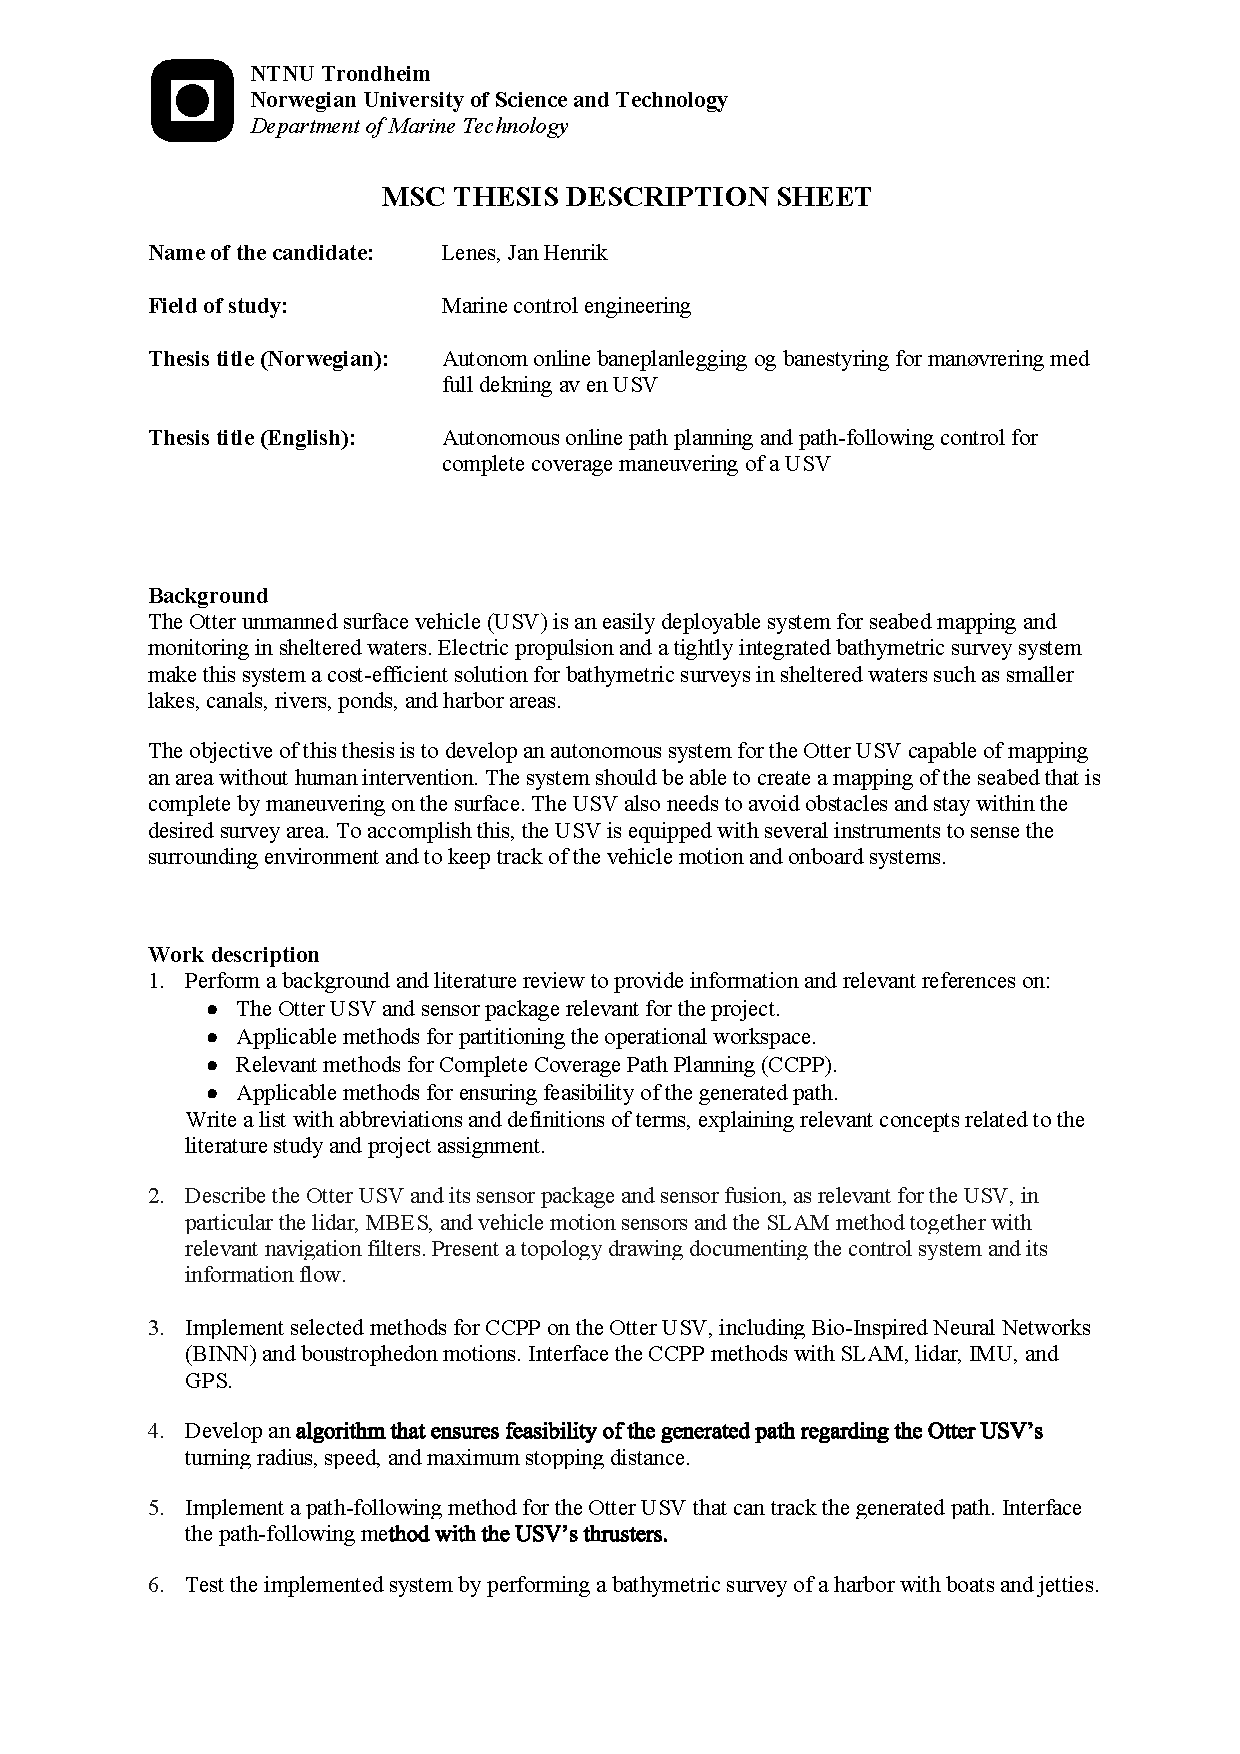
\includepdf[pages=-]{msc-desc2.pdf}

\section*{Abstract}
\thispagestyle{plain}
\addcontentsline{toc}{chapter}{Abstract}

%The cover and the title page are generated automatically when you complete your thesis (see innsida.ntnu.no/masteroppgave), so the first two pages in the thesis you submit will be the Abstract and the Sammendrag.

%Write the Abstract for your thesis here. The Abstract should fit on one page.

%Purpose, issue
Complete coverage maneuvering requires planning and following a path such that a sensor or end-effector covers every part of the workspace. The design of complete coverage paths is an essential problem in seabed mapping and many other robotic applications. The application of coverage algorithms has been very successful in land-based robots such as lawnmowers and vacuum cleaners. Independently, coverage algorithms can be classified as either offline or online. Offline algorithms assume full prior knowledge of the environment, while online algorithms rely on real-time sensor measurements.

Most complete coverage path planning (CCPP) algorithms are offline, their online use is not common, even for lawnmowers. Online CCPP approaches for marine surface vehicles are even harder to find. Existing methods for seabed mapping usually require information about the target region before the mapping can begin. To address this issue, this thesis considers the design and testing of an online complete coverage maneuvering system for seabed mapping with unmanned surface vehicles (USVs).

%Scope and Limitations
%Methods used
The proposed system uses a low-cost 2D lidar and vehicle motion sensors for simultaneous localization and mapping (SLAM). The information gathered from these onboard sensors is used by an online CCPP method in order to generate a collision-free path. Two different online CCPP methods are reviewed. One is based on a bio-inspired neural network (BINN), and the other on boustrophedon motions, also known as lawnmower patterns. The feasibility of the generated path is ensured by taking into account the USV's turning radius and speed. Finally, a line-of-sight guidance law generates continuous course and speed control to ensure that the USV tracks the generated path. 

%The main results
The proposed system has been implemented using the Robot Operating System (ROS) middleware, and is provided as open source packages. The system has been tested and verified in simulations and real-world experiments with the Otter USV. Results showed that the boustrophedon motions CCPP method performed satisfactorily, while the BINN CCPP method tended to generate inefficient paths. Methods for ensuring a feasible path and guidance managed to successfully make the Otter USV track the generated path. The proposed sensor fusion and SLAM system performed satisfactorily in certain situations, but was in general not good enough with the incorporation of IMU and GNSS data. Furthermore, the low-cost 2D lidar used in the experiments was, by itself, not capable of providing the detail necessary for accurate obstacle detection in marine environments. 

%Conclusions and recommendations
In conclusion, the proposed system performed satisfactorily and achieved complete coverage in simulations, and in real-world experiments under certain conditions. However, the sensor fusion and SLAM system did not perform satisfactorily in real-world experiments and should be improved. 

\clearpage




\begin{otherlanguage}{norsk}

\newgeometry{top=2.5cm,right=1.7in,left=1.7in,bottom=2.5cm}

\section*{Sammendrag\\[2ex]\large\normalfont{({\itshape Norwegian translation of the abstract})}}
\thispagestyle{plain}
\addcontentsline{toc}{chapter}{Sammendrag}

\noindent Manøvrering med full dekning krever planlegging og følging av en bane slik at en observasjonssensor eller robotdel dekker hele arbeidsområdet. Utformingen av baner med full dekning er et viktig problem ved kartlegging av havbunnen og mange andre anvendelser innen robotikk. Anvendelsen av dekningsalgoritmer har vært svært vellykket innen landbasert robotikk som robotstøvsugere og -gressklippere. Dekningsalgoritmer kan generelt klassifiseres som enten offline eller online. Offline algoritmer antar full forkunnskap om omgivelsene, mens online algoritmer benytter seg utelukkende av informasjon innhentet fra måleinstrumenter på roboten.

De fleste dekningsalgoritmer er offline algoritmer, selv for robotgressklippere. Online dekningsalgoritmer for marine overflatefartøy er enda vanskeligere å finne. Eksisterende metoder for kartlegging av havbunnen krever som oftest forhåndskunnskaper om området før kartleggingen kan begynne. Denne avhandlingen ønsker å løse dette problemet, og omhandler derfor utvikling og testing av et online system for manøvrering med full dekning til bruk i kartlegging av havbunnen med ubemannede overflatefartøy.

Det utviklede systemet bruker en billig 2D lidar og andre måle\-instru\-menter for posisjons- og orienteringsbestemmelse til samtidig lokalisering og kartlegging av omgivelsene. Denne informasjonen brukes videre av en online dekningsalgoritme som planlegger en kollisjonsfri bane gjennom arbeidsområdet. To forskjellige dekningsalgoritmer er vurdert. Én er basert på et bioinspirert nevralt nettverk, og den andre på å generere enkle gressklippermønster. Det ubemannede overflatefartøyets fart og svingeradius brukes til å sørge for at de genererte banene er gjennomførbare. En siktlinjebasert fartøystyringsmetode sørger til slutt for at fartøyet følger den genererte banen.

Systemet har blitt implementert ved bruk av Robot Operating System, og er publisert som åpen kildekode. Systemet har blitt testet og verifisert i simuleringer og virkelige eksperimenter med det ubemannede fartøyet Otter USV. Dekningsalgoritmen basert på gressklippermønster ga tilfredsstillende resultater, mens algoritmen basert på det bioinspirerte nevrale nettverket genererte ineffektive baner. Metodene for å sørge for gjennomførbare baner og styring av fartøyet fungerte også tilfredsstillende. Det foreslåtte systemet for fusjon av data fra måleinstrumentene var tilstrekkelig under visse forhold, men generelt ikke godt nok i inkluderingen av posisjonsdata fra GPS. Videre var ikke den billige 2D lidaren god nok for pålitelige objektdetektering i marine omgivelser.

Oppsummert så fungerte det utviklede systemet godt og oppnådde full dekning i simuleringer og under visse forhold også i virkelige eksperimenter. Metoden for fusjon av data fra måleinstrumentene fungerte imidlertid ikke godt nok og må forbedres.

\end{otherlanguage}

\restoregeometry

\clearpage


\section*{Preface}
\thispagestyle{plain}
\addcontentsline{toc}{chapter}{Preface}

This thesis was submitted to the Norwegian University of Science and Technology (NTNU) in completion of my master's degree in Engineering and ICT, with a specialization in the field of Marine Cybernetics. The work presented herein was carried out during the spring of 2019 under the guidance of Professor Roger Skjetne at the Department of Marine Technology, and in close collaboration with Maritime Robotics AS and Arild Hepsø who has been co-supervising this thesis. This work is a continuation of the work done during my specialization project in the autumn of 2018.  

\subsection*{Acknowledgments}

A huge thanks to my supervisor, Professor Roger Skjetne, for his helpful guidance and supervision. He has supported me with his great knowledge of marine control engineering, guiding me in the right direction and providing me with good ideas on how to solve the problem.

I would also like to extend my sincere gratitude to all the people at Maritime Robotics AS that have supported me. They had the idea that inspired this thesis and have been invaluable in making the project come to life. I am in particular grateful to Arild Hepsø, Stephanie Kemna, Kenan Trnka and Sindre Fossen. They have provided me with ideas, helped solve technical difficulties, and given me valuable feedback on this report.

\vspace{1.5cm}

\centerline{Trondheim, June 10th, 2019}

\vspace{1cm}

\centerline{Jan Henrik Lenes}

\clearpage

\phantomsection
\addcontentsline{toc}{chapter}{Contents}
\tableofcontents

\clearpage
\phantomsection
\addcontentsline{toc}{chapter}{List of Figures}
\listoffigures	
								
\chapter*{Abbreviations}
\addcontentsline{toc}{chapter}{Abbreviations}

\noindent 
\begin{center}
\begin{longtable}{ p{.20\textwidth} p{.80\textwidth} }
	2D/3D  & 2-Dimensional/3-Dimensional \\ 
	AHRS & Attitude and Heading Reference System \\
	ASV  & Autonomous Surface Vehicle \\
	AUV  & Autonomous Underwater Vehicle \\
	%BODY  & The body-fixed reference frame \\
	BINN  & Bio-Inspired Neural Network \\
	CCPP  & Complete Coverage Path Planning \\
	COLREGs & International Regulations for Preventing Collisions at Sea \\ 
	EKF  & Extended Kalman Filter \\
	%FOV & Field Of View \\
	GPS  & Global Positioning System \\
	GNSS & Global Navigation Satellite System \\
	IMU  & Inertial Measurement Unit \\
	INS & Inertial Navigation System \\
	Lidar & Light Detection And Ranging \\
	LOS  & Line-of-sight \\
	MBES & Multibeam Echosounder \\
	MSc & Master of Science \\
	NMEA & National Marine Electronics Association \\
	NED  & The North-East-Down coordinate system \\
	ROS  & Robot Operating System \\
	RTK & Real-Time Kinematic \\
   	SLAM  & Simultaneous Localization And Mapping \\
   	Sonar & Sound Navigation And Ranging \\
	UGV  & Unmanned Ground Vehicle \\	
	USV  & Unmanned Surface Vehicle \\
	VSLAM  & Visual Simultaneous Localization And Mapping \\
   
\end{longtable}
\end{center}

\clearpage

\pagestyle{headings}
\chapter*{Nomenclature}
\addcontentsline{toc}{chapter}{Nomenclature}

\noindent 
\begin{center}
\begin{longtable}{ p{.10\textwidth} p{.85\textwidth} p{.05\textwidth} }
	\textbf{Symbol} & \textbf{Description} & \textbf{Unit} \\\\
	$c_p$ & Coverage range in port direction. & m \\
	$c_s$ & Coverage range in starboard direction. & m \\
	$\alpha$ & Angle of detection point from the MBES. & rad \\
	$f(\alpha)$ & Distance to detection point from the MBES. & m \\	
	$r_{max}$ & Radius of circle circumscribing the USV's footprint. & m \\
	$r_i$ & Obstacle inflation radius. & m \\
	$x_w$ & The rectangular workspace's length along the x-axis. & m \\
	$y_w$ & The rectangular workspace's length along the y-axis. & m \\
	$r_c$ & Radius of circles in the circular cell partition. & m \\
	$f(r,c)$ & Flag indicating the status of a cell at row $r$ and column $c$ in the workspace partition. & 1 \\
	$e_{cell}$ & Size of cells in the square cell partition. & m \\
	$\mathbb{R}$ & The set of real numbers. & - \\
	$x_i$ & Neural activity of the $i$th neuron. & 1 \\
	$p_i$ & Position $(x_i,y_i)$ of the $i$th neuron. & (m,m) \\
	$r_0$ & Radius of the neighborhood in the neural network. & m \\
	$A$ & Passive decay rate in the neural network. & 1 \\
	$B$ & Upper bound of neural activity. & 1 \\
	$D$ & Lower bound of neural activity. & 1 \\
	$E$ & Upper and lower bound of external input to neural network. & 1\\
	$\lambda_i$ & Scaling factor for the external input to the $i$th neuron. & 1 \\
	$I_i$ & External input to $i$th neuron. & 1 \\
	$w_{ij}$ & Connection weight between the $i$th and $j$th neuron. & 1 \\
	$\mu$ & Scaling factor for connection weight between neurons. & 1 \\
	$\lambda$ & Tuning constant for how much to penalize turning in the neural network. & 1 \\
	$p_q$ & Initial position $(x_q,y_q)$ of simple Dubins path. & (m,m) \\
	$\theta_q$ & Initial heading of simple Dubins path. & rad \\
	$p_n$ & Final position $(x_n,y_n)$ of simple Dubins path. & (m,m) \\
	$\theta_n$ & Final heading of simple Dubins path. & rad \\
	$\rho$ & Turning radius in simple Dubins path. & m \\
	$\rho_{min}$ & Minimum feasible turning radius of the USV. & m \\
	$\delta$ & Turning direction. & 1 \\
	$p_c$ & Position $(x_c,y_c)$ of center of turning circle. & (m,m) \\
	$p_l$ & Position $(x_l,y_l)$ of tangent point on turning circle. & (m,m) \\
	$p$ & Position $(x,y)$ of USV. & (m,m) \\
	$p_p$ & Point $(x_p, y_p)$ on path that is closest to the USV. & (m,m) \\
	$\gamma_p$ & Path-tangential angle. & rad \\
	$y_e$ & Cross-track error. & m \\
	$\Delta(t)$ & Lookahead distance. & m \\
	$\chi$ & Course angle of the USV. & rad \\
	$\chi_d$ & Desired course angle. & rad \\
	$\tilde{\chi}$ & Error in course angle & rad \\
	$\psi$ & Heading angle of the USV. & rad \\
	$\psi_d$ & Desired heading angle. & rad \\
	$\beta$ & Sideslip angle. & rad \\
	$\Delta_{max}$ & Maximum lookahead distance. & m \\
   	$\Delta_{min}$ & Minimum lookahead distance. & m \\
   	$K_\Delta$ & Convergence rate of time-varying lookahead distance. & 1\\ 
   	$U_d$ & Desired speed. & m/s \\
   	$U_{max}$ & Maximum desired speed. & m/s\\
   	$U_{min}$ & Minimum desired speed. & m/s \\
   	$y_{max}$ & Maximum allowed cross-track error in speed assignment. & m \\
   	$\chi_{max}$ & Maximum allowed course angle error in speed assignment. & rad \\
\end{longtable}
\end{center}

\thispagestyle{plain}


\clearpage

\pagestyle{headings}

\pagenumbering{arabic} 				
\setcounter{page}{1}


\chapter{Introduction}

\section{Background}

Complete coverage maneuvering is the task of determining and following a path such that a sensor or end-effector passes over all points of an area of interest while avoiding obstacles. This is a fundamental challenge in many robotic applications, such as lawn mowing, floor cleaning, mine detection, and environmental mapping and surveying. Determining an \emph{optimal} complete coverage path, i.e. a path that covers every point exactly once, is closely related to the well-known traveling salesperson problem, which is an NP-hard problem. %\citep{Galceran2013}
This means the computational time required to solve the problem increases drastically with the size of the input. The problem becomes even more difficult to solve in unknown and dynamic environments, where reliable information about obstacles within the area of interest is not available prior to the complete coverage task.

Thus, the need arises for online approaches that solve the problem sequentially as more and more information become available through onboard sensors. These approaches operate with no prior information about the operational area, and this relaxes the requirement of covering every point exactly once. Due to the crucial role of complete coverage maneuvering in such a wide range of applications, there are several approaches reported in the literature. Applications to robotic lawnmowers and vacuum cleaners are perhaps some of the best-known examples. For references, the reader is referred to the literature review section of this thesis.

Most research in complete coverage maneuvering is targeted towards land-based applications, while the application to marine vessels, especially online approaches, is still lacking in the literature. With new developments in sensor technologies and robotics, unmanned robots are now capable of performing many tasks that previously required manned operations. This opens up for a lot of new possibilities, and the increasing popularity of autonomous systems is prominent in many sectors. The marine sector is no exception, and it is therefore important to transfer the well-established methods of land-based robotics to marine robotics.

The Otter is a small unmanned surface vehicle (USV) designed for seabed mapping and monitoring of sheltered waters, and is equipped with a multibeam echosounder (MBES) for this purpose. The Otter is a turn-key and cost-effective solution for bathymetric surveys, and Maritime Robotics has suggested implementing complete coverage maneuvering in order to increase its autonomy. To achieve this, the USV will be equipped with a low-cost 2D lidar and other vehicle motion sensors required for collision-free maneuvering on the water surface. The Otter will simultaneously keep track of obstacles on the surface with the lidar, and the covered area of the seabed with the multibeam echosounder. With this information, the USV will generate and follow collision-free paths on the surface in order to achieve complete coverage of the seabed. The Otter USV and an illustration of a bathymetric survey are shown in \figref{fig:background}.

\begin{figure}[h!]
    \centering
	\makebox[\linewidth][c]{
	\begin{subfigure}[b]{0.5\textwidth}
		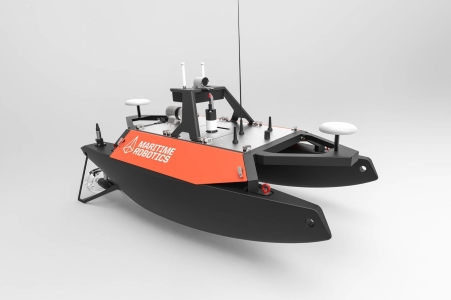
\includegraphics[width=1\linewidth]{fig/intro/otter_cgi}
		\caption{}
		\label{fig:otter}
	\end{subfigure}
	\begin{subfigure}[b]{0.5\textwidth}
		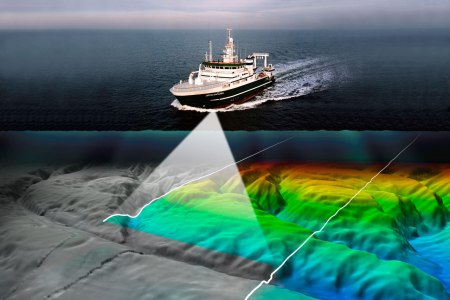
\includegraphics[width=1\linewidth]{fig/intro/seabed_mapping}
		\caption{}
		\label{fig:seabed_mapping}
	\end{subfigure}
	}
	\caption[The Otter USV and seabed mapping.]{(a) The Otter USV, courtesy of Maritime Robotics. (b) A surface vessel mapping the seabed with a multibeam echosounder, courtesy of the Marine Institute.} \label{fig:background}
\end{figure}

\section{Objective}

The main objective of this thesis is the following:

\begin{itemize}[label=\ding{212}]

\item Design, implement and test a complete coverage maneuvering system for the Otter USV using a low-cost lidar.

\end{itemize}

\noindent The system should be capable of carrying out bathymetric surveys in unknown environments without operator assistance. Based on this main objective, there are 3 subobjectives:

\begin{itemize}[label=\ding{213}]

\item Autonomous operation requires accurate real-time information about the USV and its immediate surroundings. Data from several sensors must be fused in order to accurately localize the USV. In addition, a sufficiently detailed map of the surroundings has to be provided for use in path planning.

\item A complete coverage path planning (CCPP) method must be implemented. The method should be able to generate a collision-free feasible path that ensures coverage of the desired survey area. Furthermore, this path needs to be generated online from available sensor data.

\item A guidance and path following method must be implemented. The USV must be able to follow the path generated from the complete coverage path planning method.

\end{itemize}

\noindent In order to accomplish these objectives, the author has, together with the supervisors, formulated the work description attached in the MSc thesis description in the beginning of this thesis.

\section{Thesis contributions}

The main contributions of this thesis are:

\begin{itemize}

\item A simulator for the Otter USV has been developed for ROS Melodic and Gazebo 9. The simulator implements low-level controllers and is capable of providing simulated input from several sensors, including GNSS, IMU and lidar. The simulator has been thoroughly tested and can be used for verification of methods and algorithms, including methods for SLAM, sensor fusion, path planning, guidance and path following.

\item A strategy for sensor fusion and simultaneous localization and mapping (SLAM) with Cartographer. The implemented system fuses data from GNSS, IMU and 2D lidar to provide localization and mapping of the surrounding environment.

\item A map processing strategy and two methods for partitioning of the operational workspace. One of them is particularly suited for variable coverage range sensors.

\item Two online CCPP methods. Obstacle avoidance is performed in both methods using a 2D lidar. One of the methods applies a variable inter-lap spacing, which to the author's knowledge has not yet been done in an online CCPP method for seabed mapping with obstacle avoidance. 

\item A method that ensures feasibility of the generated path regarding the Otter USV's turning radius and speed.

\item A path following method for the USV that can track the generated path.

\item An interface to Maritime Robotics' onboard system on the Otter USV for controlling the USV's thrusters from ROS.

\end{itemize}

\noindent All implementations are written in C++ for ROS Melodic and are available in the electronic attachment of this thesis, as well as on the author's GitHub page: \url{https://github.com/jhlenes/complete_coverage} and \url{https://github.com/jhlenes/usv_simulator}. These code repositories provide a good starting point and reference for further work with the Otter USV or other development in ROS.

\section{Scope and limitations}

%\todo[inline]{Scope and delimitations that emerge from the research question and objectives must be clearly explained in a separate section.}

\subsection{Outline}

The thesis is organized as follows:\vspace{0.4em}

\noindent \textbf{Chapter 2:} Provides background information and literature references on relevant topics and theory. This includes the Otter USV and its sensor package, workspace partitioning, relevant CCPP methods, and feasible path design. 
\vspace{0.4em}

\noindent \textbf{Chapter 3:} Presents the problem formulation which further defines the problem to be solved. The problem is broken down and formulated as several subproblems that can be solved individually.
\vspace{0.4em}

\noindent \textbf{Chapter 4:} Describes which sensors are necessary, how sensor data is gathered and how it is fused together with data from other sensors. The SLAM system Cartographer is introduced.
\vspace{0.4em}

\noindent \textbf{Chapter 5:} Presents how the SLAM map is processed and partitioned to represent the workspace in a way suitable for CCPP.
\vspace{0.4em}

\noindent \textbf{Chapter 6:} Describes in detail how the CCPP methods work. This includes how the underlying workspace representation is used, which strategies to use in the path planning, how to ensure complete coverage, and how to generate the waypoints.
\vspace{0.4em}

\noindent \textbf{Chapter 7:} Presents how feasible paths are generated from waypoints. A line-of-sight (LOS) guidance law for curved paths that generates continuous steering control capable of tracking these paths is also covered.
\vspace{0.4em}

\noindent \textbf{Chapter 8:} Presents results of simulations with sensor fusion and SLAM, CCPP and path following. The results are discussed with regards to reliability and performance.
\vspace{0.4em}

\noindent \textbf{Chapter 9:} Presents results of real-world experiments with the Otter USV in the harbor of Trondheim. The results are discussed with regards to reliability and performance.
\vspace{0.4em}

\noindent \textbf{Chapter 10:} Presents concluding remarks regarding the implemented system. Recommendations and suggestions for further work are also presented.
\vspace{0.4em}

\subsection{Limitations}

Some of the limitations of the implemented system are:

\begin{itemize}

\item No distinction is made between moving and stationary obstacles. This may result in some undesirable behavior regarding moving obstacles. The system is not in compliance with the Convention on the International Regulations for Preventing Collisions at Sea (COLREGs).

\item The system is only tested in simulations and experimentally in a harbor. Different environments might offer other challenges not accounted for.

\item The system has not been tested experimentally with a multibeam echosounder. Varying depth is only considered in simulations.

\item The Otter USV already has low-level control developed by Maritime Robotics. Thus, the implemented system will restrict itself to high-level planning and provide course and speed control as input to the existing onboard system.

\item A low-cost 2D lidar is the only range-based sensor, obstacles outside the lidar's scan plane are not detected.

\end{itemize}



\chapter{Background and literature review}

\section{The Otter USV and its sensor package}

Being able to sense the surrounding environment is crucial for any autonomous robot. In maneuvering, taking the appropriate action is highly dependent on having up-to-date and accurate information about the surroundings. The USV's sensors is what translates the environmental conditions into signals suitable for processing. Selecting the proper sensors is therefore critical, as it directly affects the quality of environmental information available, and consequently the maneuvering performance. This section will present the Otter USV and the sensors that are used in order to sense the surrounding environment and localize the USV.

\subsection{The Otter USV}

The experimental platform used in this thesis is the Otter USV \citep{website:MR}, an easily deployable system for bathymetric surveys developed by Maritime Robotics. The USV has a small footprint of $200$ x $105$ x $\SI{85}{\cm}$ and a weight of about $\SI{95}{\kilogram}$. It has a typical operating speed of about $\SI{2}{knots}$, and is propelled by a set of dual electrical fixed thrusters. The USV's stable catamaran design offers a payload capacity capable of supporting a multitude of different sensor configurations. The Otter USV is depicted in \figref{fig:experimental_platform}. 

\begin{figure}[h!]
    \centering
	\makebox[\linewidth][c]{
	\begin{subfigure}[b]{0.5\textwidth}
		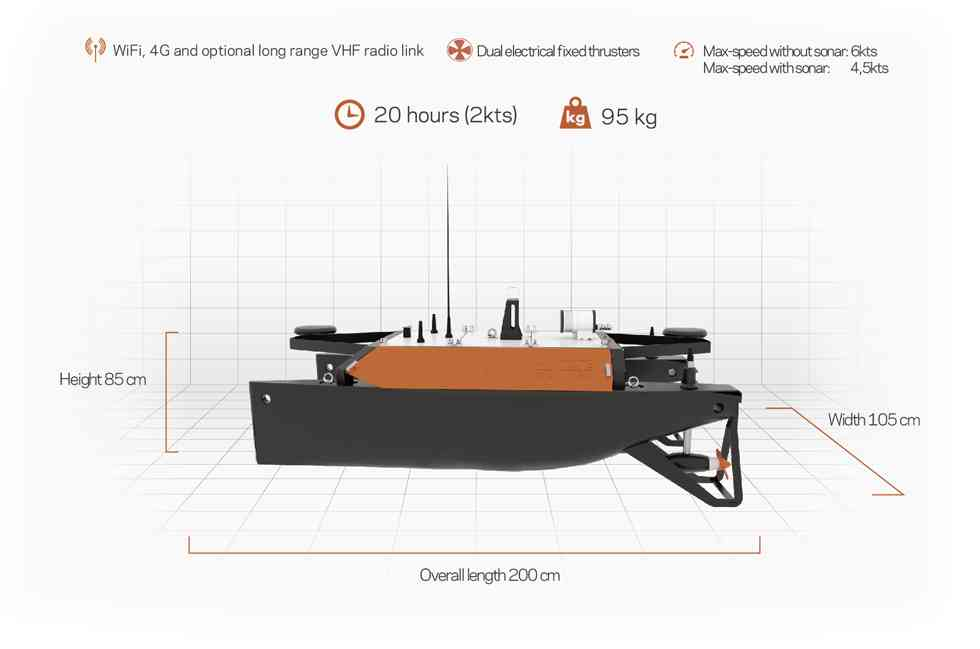
\includegraphics[width=1\linewidth]{fig/lit_rev/infographics.jpg}
		\caption{}
		\label{fig:infographics}
	\end{subfigure}
	\begin{subfigure}[b]{0.5\textwidth}
		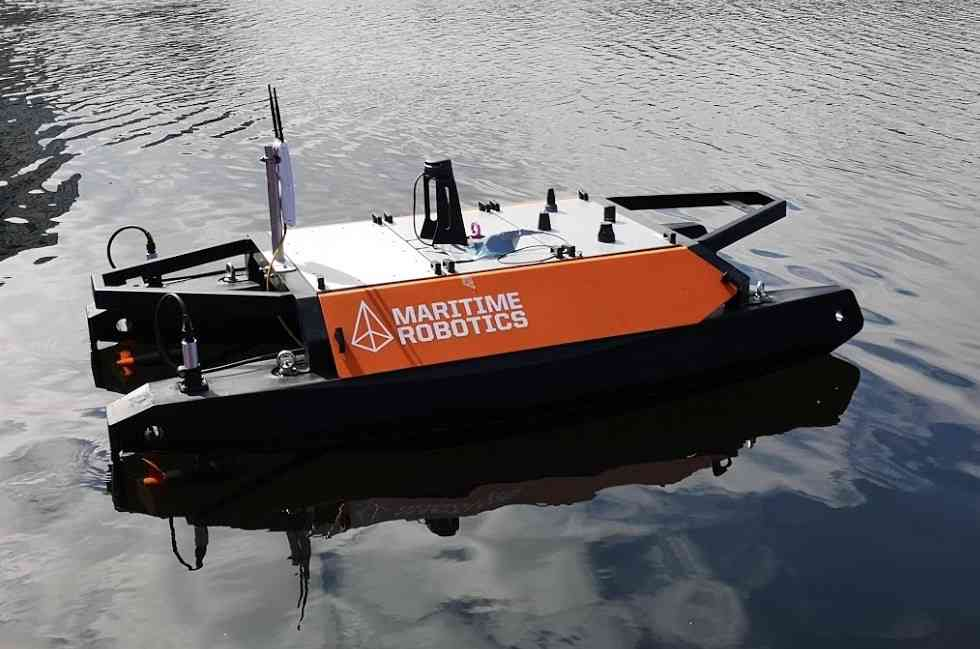
\includegraphics[width=1\linewidth]{fig/lit_rev/otter1}
		\caption{}
		\label{fig:otter_with_lidar}
	\end{subfigure}
	}
	\caption[Specifications of the Otter USV.]{(a) Specifications of the Otter USV, courtesy of Maritime Robotics. (b) The Otter USV equipped with a lidar in Trondheim harbor.} \label{fig:experimental_platform}
\end{figure}

\subsection{Relevant sensors}

\subsubsection{Lidar}

Lidar (also called LIDAR or LiDAR) stands for light detection and ranging, and is a method that uses light to measure the distance to a target \citep{wiki:lidar}. This is done by emitting laser pulses and measuring the time it takes for the pulse to be reflected. Measuring the distance in a wide range of directions allow lidars to make accurate and precise depictions of the surroundings, as illustrated in \figref{fig:lidar}.

\begin{figure}[h!]
    \centering
	\makebox[\linewidth][c]{
	\begin{subfigure}[b]{0.5\textwidth}
		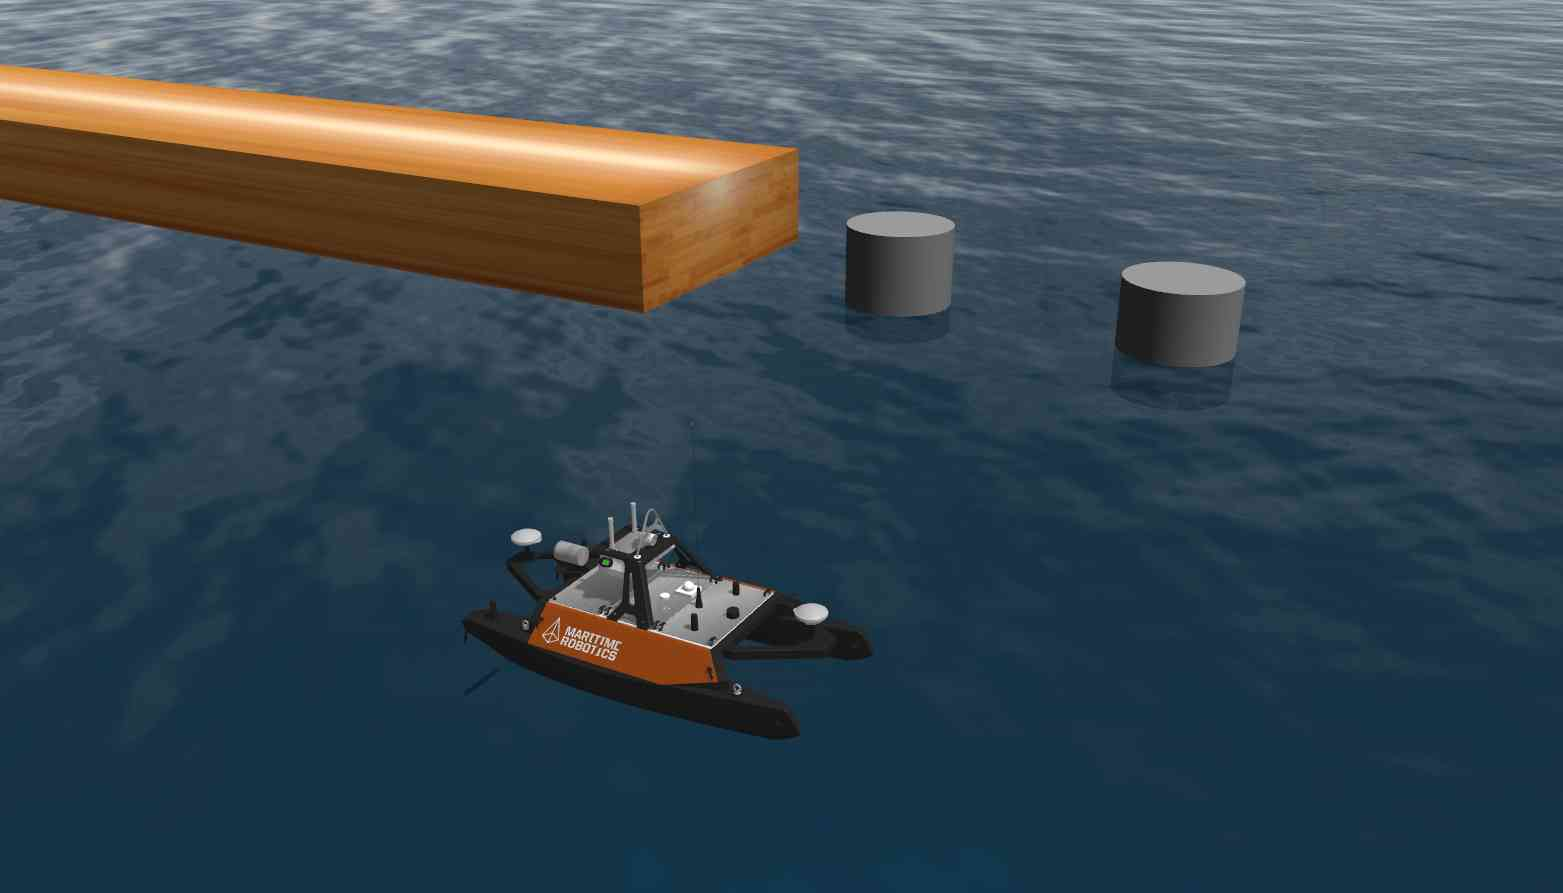
\includegraphics[width=1\linewidth]{fig/lit_rev/lidar_sim.jpg}
		\caption{}
		\label{fig:lidar_rays}
	\end{subfigure}
	\begin{subfigure}[b]{0.5\textwidth}
		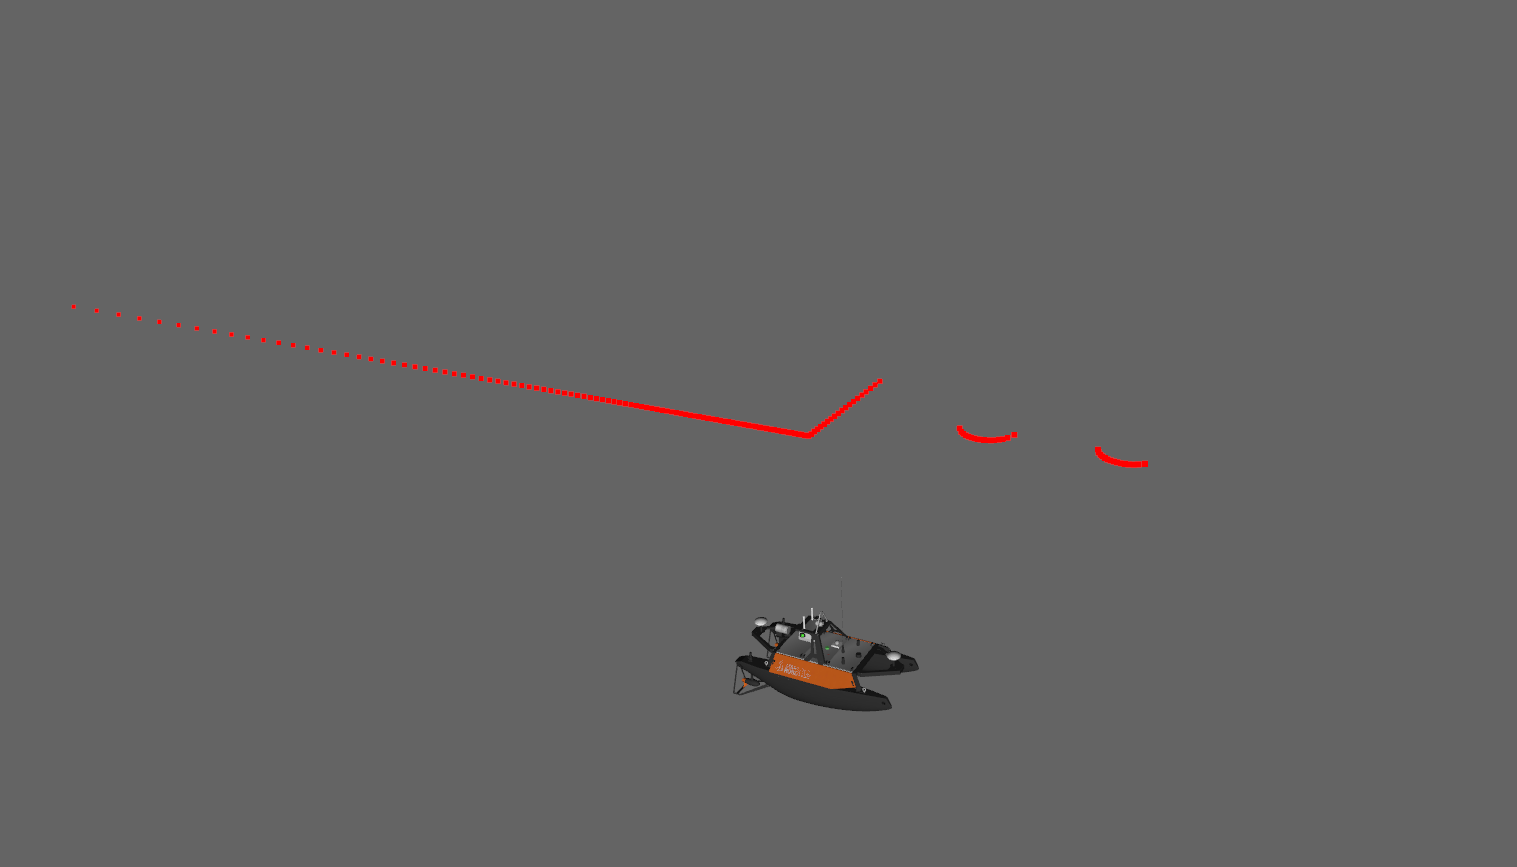
\includegraphics[width=1\linewidth]{fig/lit_rev/lidar_scan}
		\caption{}
		\label{fig:lidar_scan}
	\end{subfigure}
	}
	\caption[Illustration of a laser scan.]{(a) The USV in a simulated environment with obstacles. (b) The laser scan created by the lidar depicts an accurate mapping of the surroundings.}
	\label{fig:lidar}
\end{figure}

The range, resolution, and field of view vary a lot between different types of lidars. However, even low-cost 2D lidars can be used for navigation, for example in vacuum cleaners such as the Roborock S6 \citep{website:roborock}. A low-cost 2D lidar was also used successfully by \citet{Ueland2016} on a marine vessel to explore and navigate in a basin with unknown obstacles. A significant drawback of 2D lidars is that obstacles that occur either above or below the sensor's horizontal scan plane will not be detected. To account for this issue, \citet{Spange2016} incorporated the use of acoustic proximity sensors, which solves the issue inside the range of the proximity sensors. Both of the works by \citet{Spange2016} and \citet{Ueland2016} were performed in a basin where the lidar was largely unaffected by roll and pitch motions caused by waves.

Examples of better and more expensive 2D lidars are those in use on the multipurpose unmanned ground vehicles (UGVs) by Clearpath robotics \citep{website:Clearpath}. Compared to the cheaper lidars, these usually offer a significant increase in range, resolution and outdoor availability. State-of-the-art 3D lidars offer even more detailed depictions of the surrounding environment and avoid the issue of a single scan plane as in 2D lidars, but at the cost of a significant price increase. High-end lidars like this can be used in applications where the requirements to accuracy and precision are incredibly high, such as terrain mapping and self-driving cars. See for instance the Velodyne Puck \citep{website:VLP} and the YellowScan Surveyor \citep{website:YellowScan} lidars.

%% which to buy?
%The Otter USV does not require a very detailed mapping of the environment, it just needs enough detail to be able to detect large obstacles (like boats and jetties) and avoid them. Keeping the costs of the USV to a minimum is also of interest. Consequently, only low-cost 2D lidars are relevant when considering the sensor suite for the USV. Many 2D lidars are intended mainly for indoor use, and therefore have rather limited ranges and poor performance in sunlight. The 2D lidars from Hokuyo are examples of this, e.g. the Hokuyo URG-04LX-UG01 \citep{website:Hokuyo}. A low-cost 2D lidar which combines both a reasonable range and outdoors availability, is the RPLIDAR from SLAMTEC \citep{website:Slamtec}. This lidar is the Otter USV's main source of information about the surrounding environment.

\subsubsection{IMU}

An inertial measurement unit (IMU) is a device that measures the angular rate, force and sometimes magnetic field \citep{wiki:imu}. There are three main types of motion sensor devices in an IMU, and that is an accelerometer, gyroscope, and magnetometer. IMUs often contain some software that combines these measurements in order to provide orientation and heading, resulting in an attitude and heading reference system (AHRS). If the IMU has software that also calculates the position relative to a global reference frame, it is often called an inertial navigation system (INS) \citep{wiki:ins}. As with lidars, IMUs come with varying quality. Examples of cheap IMUs are the ones from SparkFun Electronics \citep{website:sparkfun}, while the very accurate POS MV \citep{website:applanix} system from Applanix is a much more accurate and expensive solution.

\subsubsection{GNSS}

Global navigation satellite system (GNSS) is a navigation system that uses satellites to provide geo-spatial positioning \citep{wiki:gnss}. GNSS allows small electronic receivers to determine their latitude, longitude, and altitude/elevation with high precision (within a few meters) using positioning and timing data transmitted from satellites. Popular publicly available GNSS systems include GPS, GLONASS, and Galileo. GNSS receivers are found many places such as in phones and watches, and are readily available at many online electronics stores \citep{website:sparkfun}. With more advanced RTK GNSS solutions, the precision of GNSS positioning can be increased to centimeter level accuracy \citep{wiki:rtk}, which is often important in applications such as land surveys and hydrographic surveys.

\subsubsection{MBES}

A multibeam echosounder (MBES) is a type of downward-looking sonar that is frequently used to map the seabed \citep{wiki:mbes}. The MBES is usually mounted on a ship's hull, and emits sound waves in a fan shape beneath the ship. The time it takes for the sound waves to bounce off the seabed and return to a receiver on the MBES, is used to determine water depth. This gives an accurate depiction of the seabed directly beneath the ship, see \figref{fig:mbes}.

\begin{figure}[h!]
    \centering
	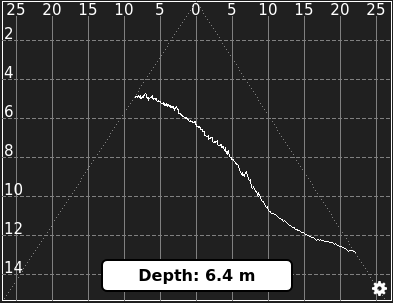
\includegraphics[width=0.5\linewidth]{fig/lit_rev/mbes}
	\caption[Multibeam echosounder measurement of the seabead.]{A multibeam echosounder measures the depths in a swath beneath the ship. Visualized by Maritime Robotics' Vehicle Control Station.}
	\label{fig:mbes}
\end{figure}

There are several use cases for multibeam echosounders, and the field of view, depth range and resolution vary accordingly. The NORBIT iWBMS is an example of a compact and high resolution sonar for shallow water mapping, and can operate in depth ranges of $0.2$ -- $275$ meters \citep{website:norbit}. Other sonars, like the Kongsberg Maritime EM 124 are meant to operate at full ocean depths, and can handle depth ranges of $20$ - $11000$ meters \citep{website:km}.

\section{Partitioning of the operational workspace}

The operational workspace of a robot is the space in which the robot is operating. In the case of the Otter USV, the workspace is the reachable portion of the desired survey area. Partitioning the workspace then becomes the task of splitting the workspace into smaller, more manageable regions that are better suited for path planning. The choice of a partitioning strategy is an important part of CCPP, and is therefore given a thorough review here.

%The survey \citep{Galceran2013} summarizes many partitioning methods for CCPP.

\subsection{Grid-based decomposition}

In grid-based decomposition, the workspace is decomposed into a collection of uniform cells ordered in a grid. In this representation, each cell represents a small region of space in the real world, and is usually the size of the robot's footprint, end-effector, or observation sensor's coverage range. This makes it very suitable for CCPP, because when all cells in the grid are covered, complete coverage is achieved. Grid-based decomposition is, however, an approximate representation of the workspace. If the area a cell represents is only partially covered by an obstacle in the real world, the entire cell is often considered as an obstacle. Some grid-based decomposition methods are illustrated in \figref{fig:grid_shapes}.

\begin{figure}[h!]
    \centering
	\makebox[\linewidth][c]{
	\begin{subfigure}[t]{0.5\textwidth}
		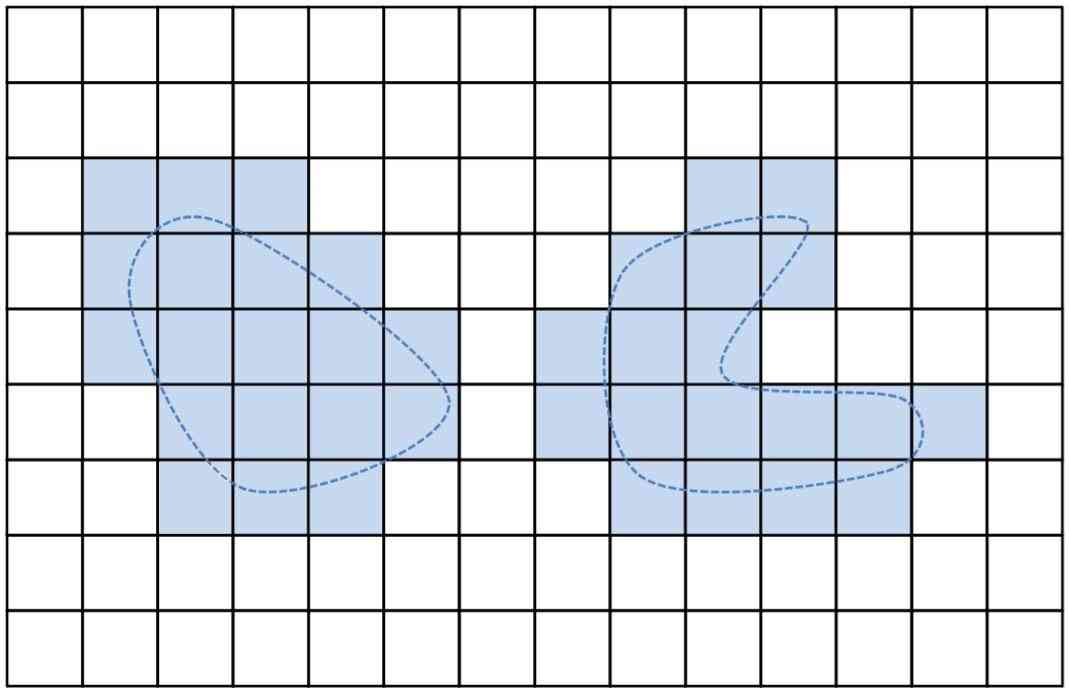
\includegraphics[width=1\linewidth]{fig/lit_rev/square_cell1}
		\caption{Square cell decomposition \citep{Galceran2013}. Obstacles are outlined by the dashed lines, and the colored cells are considered obstacles.}
		\label{fig:grid_square}
	\end{subfigure}
	\quad
	\begin{subfigure}[t]{0.5\textwidth}
		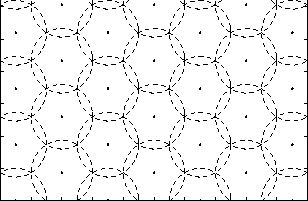
\includegraphics[width=1\linewidth]{fig/lit_rev/circular_cell}
		\caption{Circular disk decomposition \citep{guo2004coverage}.}
		\label{fig:grid_circular}
	\end{subfigure}
	}
	\makebox[\linewidth][c]{
	\begin{subfigure}[t]{0.5\textwidth}
		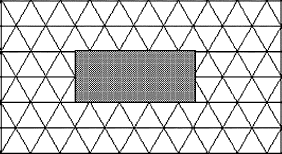
\includegraphics[width=1\linewidth]{fig/lit_rev/triangular_cell}
		\caption{Triangular cell decomposition \citep{oh2004complete}. Colored rectangle represents obstacles.}
		\label{fig:grid_triangular}
	\end{subfigure}
	}
	
	\caption{Grid-based decomposition methods.}
	\label{fig:grid_shapes}
\end{figure}

Many CCPP methods use a grid-based decomposition in their partitioning of the workspace. The grid cells are often square, as in the methods by \citet{Viet2013} and \citet{yang2004neural}. However, other shapes are also used, such as circular disks \citep{guo2004coverage} and triangles \citep{oh2004complete}. Decomposition into circular disks with the coverage range as the radius of the circles, is motivated by the fact the it will sometimes give a more correct representation of the covered area compared to squares. Circular disk decomposition has been used in several CCPP methods, such as \citet{guo2006complete} and \citet{Scibilia2012}. The triangular cells used by \citet{oh2004complete} offers an advantage over other shapes in that each cell has 12 neighboring cells, resulting in more directions for movement between neighboring cells.

An advantage of grid-based decomposition, is that a grid-map is easy to create and maintain in an implemented system. It is easily represented in a simple array-structure, which most programming languages have access to. One of the downsides of grid-based decomposition is that it is approximate, and most CCPP methods using grids are therefore resolution-complete \citep{Galceran2013}. That is, the completeness of the methods depend on the resolution of the grid map, as seen in \figref{fig:grid_square}. Another disadvantage is that the requirement to memory becomes large in big workspaces with very small cell sizes. Grid-based decomposition also requires accurate localization and mapping in order to be able to distinguish between adjacent grid cells.

%This is because grid-based approaches require a resolution accurate enough to capture the most important details of the world \citep{thrun1998learning}.

\subsection{Morse-based cellular decomposition}

%See here: \citep{Galceran2013}.

\citet{acar2002morse} introduced the term Morse decompositions as a class of exact cellular decomposition whose cells have a simple structure that can be readily covered. In Morse-based cellular decomposition, the workspace is partitioned into non-overlapping cells that, together, exactly cover the workspace. Thus, exact cellular decomposition. The cells themselves are created based on critical points of Morse functions. By choosing different functions, different cell shapes are obtained. These cells are not uniform in size or shape as in grid-based partitioning, but rather shaped such that each cell itself can be covered by a simple motion. An example of a simple motion is the boustrophedon motion, i.e. a simple back-and-forth lawnmower pattern. Complete coverage is then achieved by covering each individual cell with a simple motion.



The chosen Morse function defines what Acar terms a slice function, and this slice is swept through the target space. When the sweep line encounters an obstacle with a surface normal perpendicular to the sweep line, a critical point is found. A vertical sweep line results in a boustrophedon decomposition \citep{choset2000exact}. \figref{fig:morse_crit} shows the online detection of a critical point and thus the edge of a cell. \figref{fig:morse_cells} shows a complete exact cell decomposition of a workspace.

\begin{figure}[h!]
    \centering
	\makebox[1.0\linewidth][c]{
	\begin{subfigure}[t]{0.5\textwidth}
		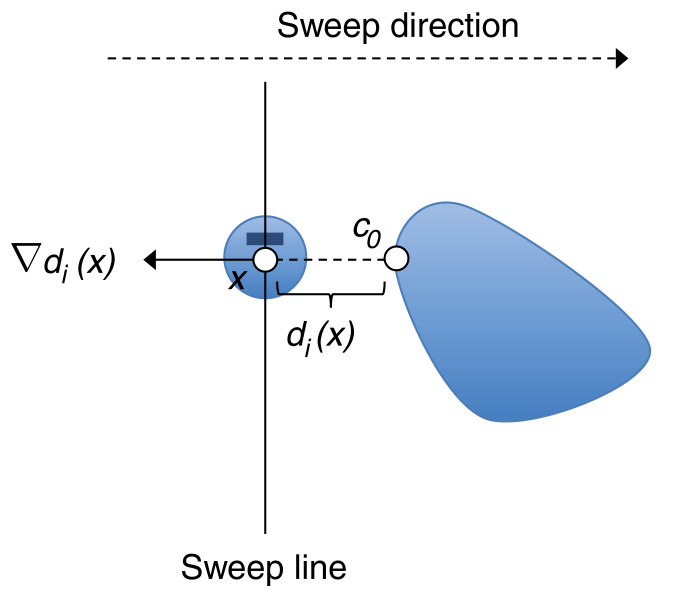
\includegraphics[width=1\linewidth]{fig/lit_rev/morse_crit}
		\caption{A critical point detected by a robot moving along the sweep line \citep{Galceran2013}.}
		\label{fig:morse_crit}
	\end{subfigure}
	\quad
 	\begin{subfigure}[t]{0.5\textwidth}
		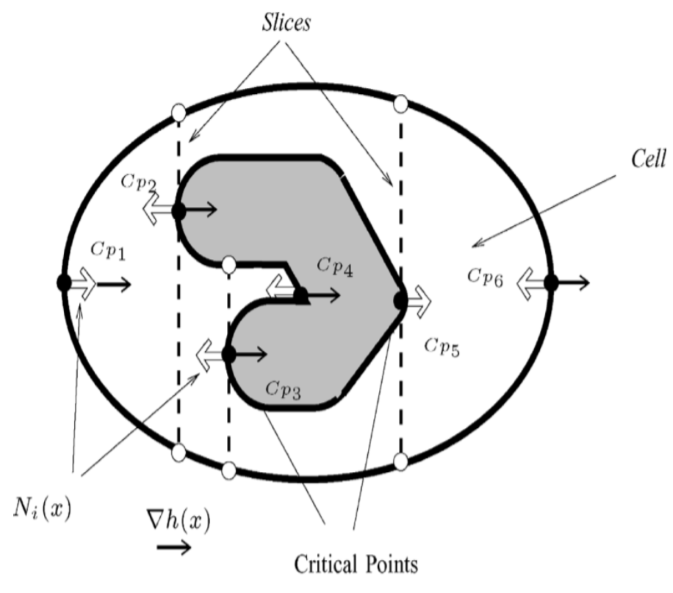
\includegraphics[width=1\linewidth]{fig/lit_rev/morse_cells}
		\caption{Cell decomposition of a workspace \citep{acar2006sensor}.}
		\label{fig:morse_cells}
	\end{subfigure}
 	}
	\caption{Morse-based cellular decomposition with a vertical sweep line.}
	\label{fig:morse_decomp}
\end{figure}

The CCPP method by \citet{acar2002sensor} is an example of a method that uses Morse-based cellular decomposition. This is an online method that, upon the detection of critical points while moving through the workspace, creates and modifies cells. \citet{acar2006sensor} takes this approach one step further by combining Morse-based cellular decomposition with generalized Voronoi diagrams. The Voronoi diagrams are used for representing narrow or cluttered spaces, while Morse-based cellular decomposition is used for open spaces. This allows for more efficient coverage for certain types of robots and applications.

\section{Relevant methods for CCPP} \label{sec:lit-rev-ccpp}

There are some works in the literature that address the problem of CCPP for seabed coverage. \citet{galceran2013planning} is an offline CCPP method for AUVs that takes a bathymetric map as input and generates complete coverage paths for in-detail inspections of the ocean floor. \citet{williams2010optimal} detects underwater mines with an AUV by covering an area by parallel tracks with varying track-spacing. Another method by \citet{paull2013sensor} considers online CCPP for mine countermeasures with AUVs. These methods all operate on AUVs, and their main focus is on effective mapping of the seabed. However, online obstacle avoidance is not considered in any of them.

\citet{galceran2012efficient} proposed an efficient offline method for ASVs and AUVs that minimizes the amount of coverage overlap. Given a prior depth map, the method starts by segmenting the target area into regions of similar depth. Each of these regions are then handled as a separate coverage problem and, assuming no obstacles in the region, covered with simple parallel back-and-forth laps. Since the spacing between each lap is constrained by the shallowest point on the surface, the similar-depth regions reduce the coverage overlap. They further reduce coverage overlapping by choosing a sweeping direction inside each of these regions that is oriented perpendicular to the seafloor surface gradient, thus minimizing the difference between the shallowest and deepest point in one lap. Lastly, the inter-lap spacing is maximized on a lap-by-lap basis where the spacing is determined by the shallowest point on the current lap. The complete coverage paths generated by this method is shown in \figref{fig:galceran_ccpp}.

\begin{figure}[h!]
    \centering
	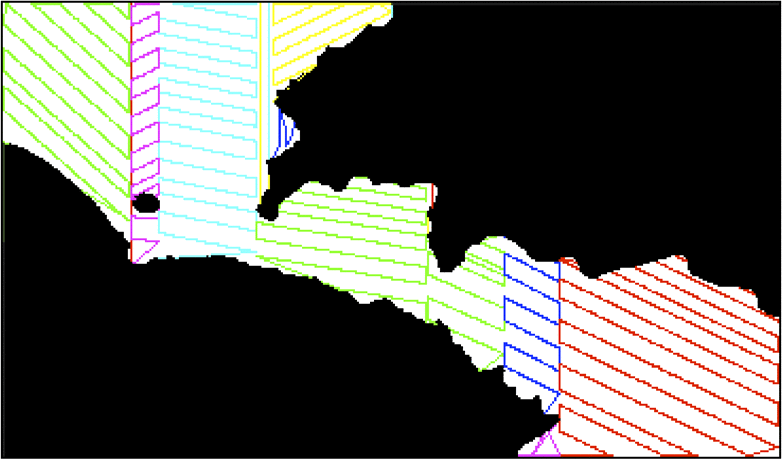
\includegraphics[width=0.5\linewidth]{fig/lit_rev/galceran_ccpp}
	\caption[Complete coverage paths for regions segmented by similar depth.]{Complete coverage paths for regions segmented by similar depth \citep{galceran2012efficient}.}
	\label{fig:galceran_ccpp}
\end{figure}

Most CCPP methods are developed for use with fixed size sensors or end-effectors, such as those found in vacuum cleaners, lawnmowers or painting robots. The comprehensive survey by \citet{Galceran2013} reviews many of these, and most of them use some sort of boustrophedon motions. Other methods, like \citet{yang2004neural} and \citet{Scibilia2012}, use a topologically organized neural network to plan the paths. While these methods do not address the topic of seabed mapping with a variable coverage range sensor, they do address the problem of obstacle avoidance in unknown environments. One method that makes use of boustrophedon motions, is the BA* method described in \citet{Viet2013}. In this method, the operational workspace is partitioned into uniform square grid cells. The method constructs boustrophedon motions by moving between cells in a north-south-east-west priority. When the robot gets stuck, it uses an A* search to backtrack to another starting point where a new boustrophedon motion is started. The paths generated by the method is shown in \figref{fig:ba_star}. 

\begin{figure}[h!]
    \centering
	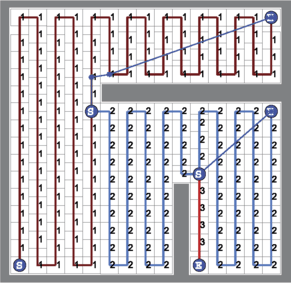
\includegraphics[width=0.5\linewidth]{fig/lit_rev/ba_star}
	\caption[Complete coverage with boustrophedon motions and backtracking with A* search.]{Complete coverage with boustrophedon motions and backtracking with A* search \citep{Viet2013}.}
	\label{fig:ba_star}
\end{figure}

\section{Feasible path design}

Most CCPP methods generate paths as waypoints, or as straight-line segments between waypoints. This is perfectly fine for robotic applications where the cost of repeatedly starting, stopping and in-place turning is low, such as lawn mowing and floor cleaning. For other applications, especially those involving underactuated USVs, this is far less favorable due to an increase in factors such as power consumption and time duration. In these cases, it is desirable with a feasible path that takes into account the kinematic constraints of the robot.

Connecting points with feasible paths can be achieved in several ways, each with its own advantages and disadvantages. The different approaches can usually be distinguished into two main categories: combining straight lines and arc segments, or using splines \citep{lekkas2014guidance}. % In this thesis, straight lines and arc segments are used. 
The main disadvantage of using straight lines and arc segments is the curvature discontinuity which occurs between two consecutive path segments. On the other hand, the constant curvature of these paths allows for smaller variations in the control outputs compared to splines. Splines are smooth, but have an always varying curvature which means the control output is changing all the time.

%Moving on straight lines and arc segments also means fewer zig-zag turns between points, ensuring a more stable course. This is an advantage in applications like seabed mapping, where an accurate course estimate is important for the quality of measurements.

\subsection{Polynomial approximation}

\citet{guo2006complete} proposed an approach for polynomial approximation using a rolling window of six waypoints, see \figref{fig:poly_approx}. A smooth path is sequentially generated between the third and fourth waypoint. Consequently, this method requires planning at least three waypoints ahead in time. The approach generates three cubic polynomials from the first four points, middle four points, and last four points. These three polynomials are then used to obtain the first and second derivatives of the line-segment between the third and fourth waypoint. These, in turn, can be used as boundary conditions in order to obtain a fifth order polynomial which connects the third and fourth waypoint. Consequently, the resulting path is guaranteed to have continuous second-order derivatives.

\begin{figure}[h!]
    \centering
	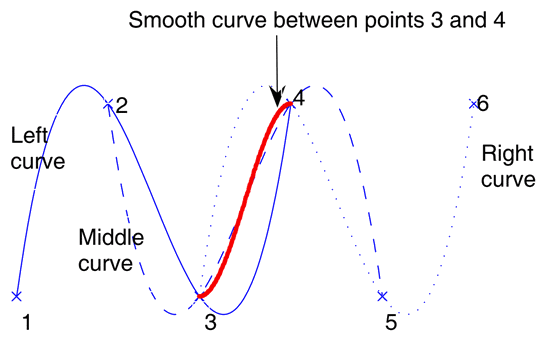
\includegraphics[width=0.5\linewidth]{fig/lit_rev/poly_approx}
	\caption[Polynomial approximation of a 6-point rolling window.]{Polynomial approximation of a 6-point rolling window \citep{guo2006complete}.}
	\label{fig:poly_approx}
\end{figure}

\subsection{Dubins path}

Dubins path is the shortest path for a Dubins vehicle between two points with a constraint on average curvature, and with prescribed initial and terminal positions and tangents \citep{dubins1957curves}. Dubins vehicle is defined as a non-holonomic vehicle that is constrained to move along planar paths of bounded curvature, and can only travel forward along the path. The generated Dubins path is composed only of circular arcs and line segments as shown in \figref{fig:dubins_path}. By using a robot's minimum turning radius in the generation of the Dubins path, the feasibility of the path is guaranteed.

\begin{figure}[h!]
    \centering
	\makebox[1.0\linewidth][c]{
	\begin{subfigure}[t]{0.5\textwidth}
		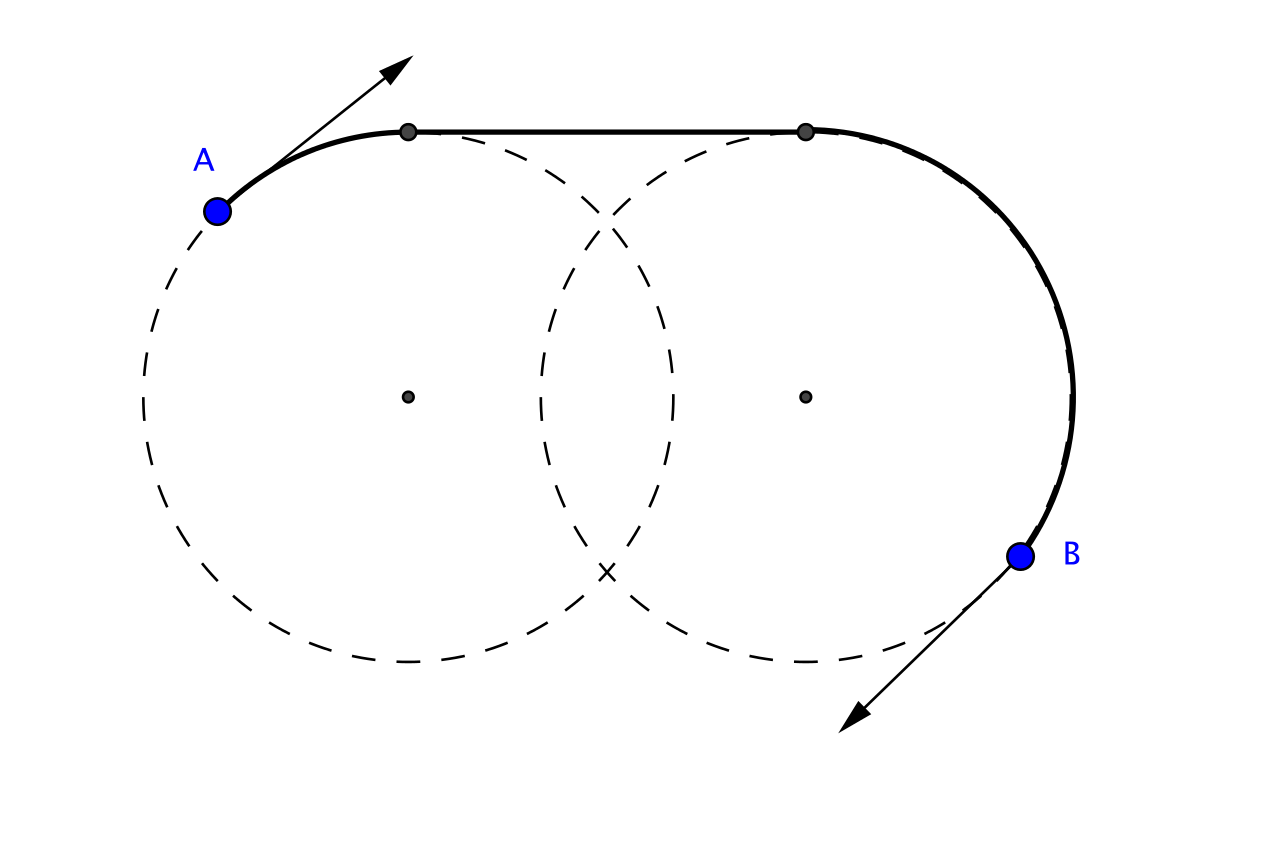
\includegraphics[width=1\linewidth]{fig/lit_rev/dubins1}
		\caption{}
		\label{fig:dubins1}
	\end{subfigure}
	\quad
 	\begin{subfigure}[t]{0.5\textwidth}
		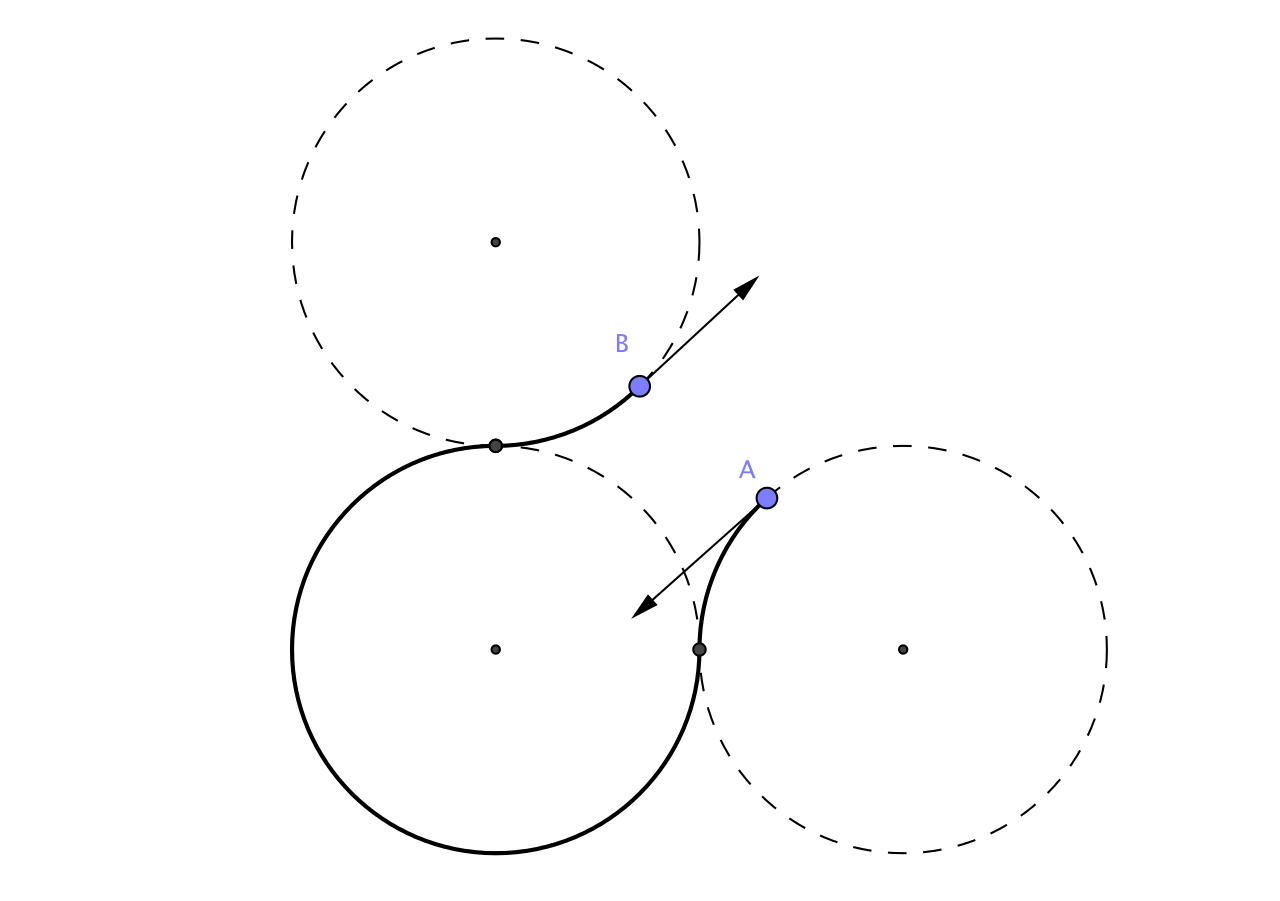
\includegraphics[width=1\linewidth]{fig/lit_rev/dubins2}
		\caption{}
		\label{fig:dubins2}
	\end{subfigure}
 	}
	\caption[Dubins path.]{Dubins path, courtesy of Wikipedia.}
	\label{fig:dubins_path}
\end{figure}

The guidance system proposed by \citet{Scibilia2012} generates feasible paths for AUVs by using what is referred to as simple Dubins paths. By removing the constraint on the terminal heading of a Dubins path, the path is simplified considerably. The path can further be simplified by requiring a minimum feasible turning radius that is smaller than half the distance between the start and end point. The shortest path can then be described by what is referred to as a simple Dubins path, i.e. a single turn followed by a straight-ahead movement. A simple Dubins path is shown in \figref{fig:simple_dubins_path}, the terminal heading is determined from the path.


\begin{figure}[h!]
	\centering
	\makebox[1.0\linewidth][c]{
	\begin{subfigure}[t]{0.5\textwidth}
		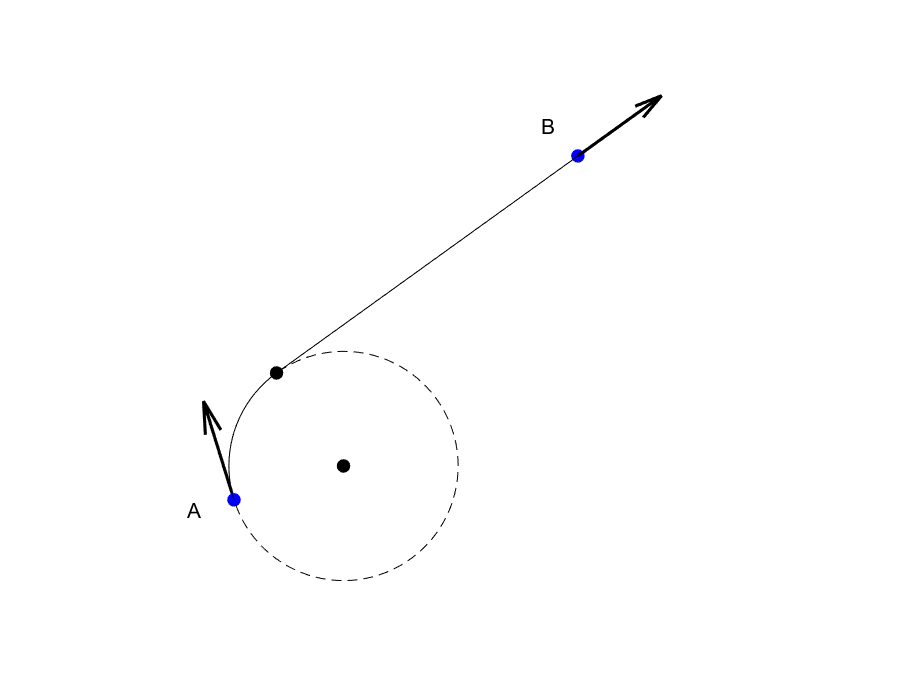
\includegraphics[width=1\linewidth]{fig/lit_rev/simple_dubins_path}
		\caption{}
		\label{fig:simple_dubins1}
	\end{subfigure}
	\quad
 	\begin{subfigure}[t]{0.5\textwidth}
		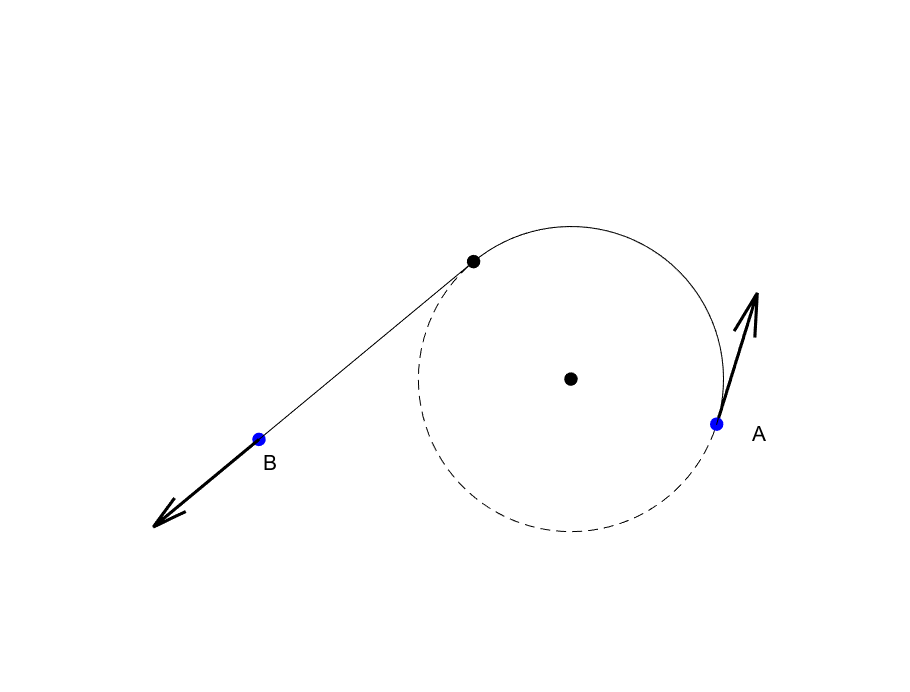
\includegraphics[width=1\linewidth]{fig/lit_rev/simple_dubins_path2}
		\caption{}
		\label{fig:simple_dubins2}
	\end{subfigure}
 	}
	\caption{Simple Dubins path.}
	\label{fig:simple_dubins_path}
\end{figure}


\subsection{Bezier curves}

Bezier curves are defined by a set of control points, but the curve itself does not pass through these points, as shown in \figref{fig:bezier_curve}. Bezier curves have several interesting and useful properties for path planning \citep{choi2008path}. For instance, together the control points define a polygon, and the Bezier curve will always be contained within the convex hull of this polygon. Another useful property is that the first and last points on the curve are coincident with the first and last control points. Furthermore, the tangents of the curve at these points are also coincident with the first and last line segments generated by subsequent control points. 

\begin{figure}[h!]
	\centering
	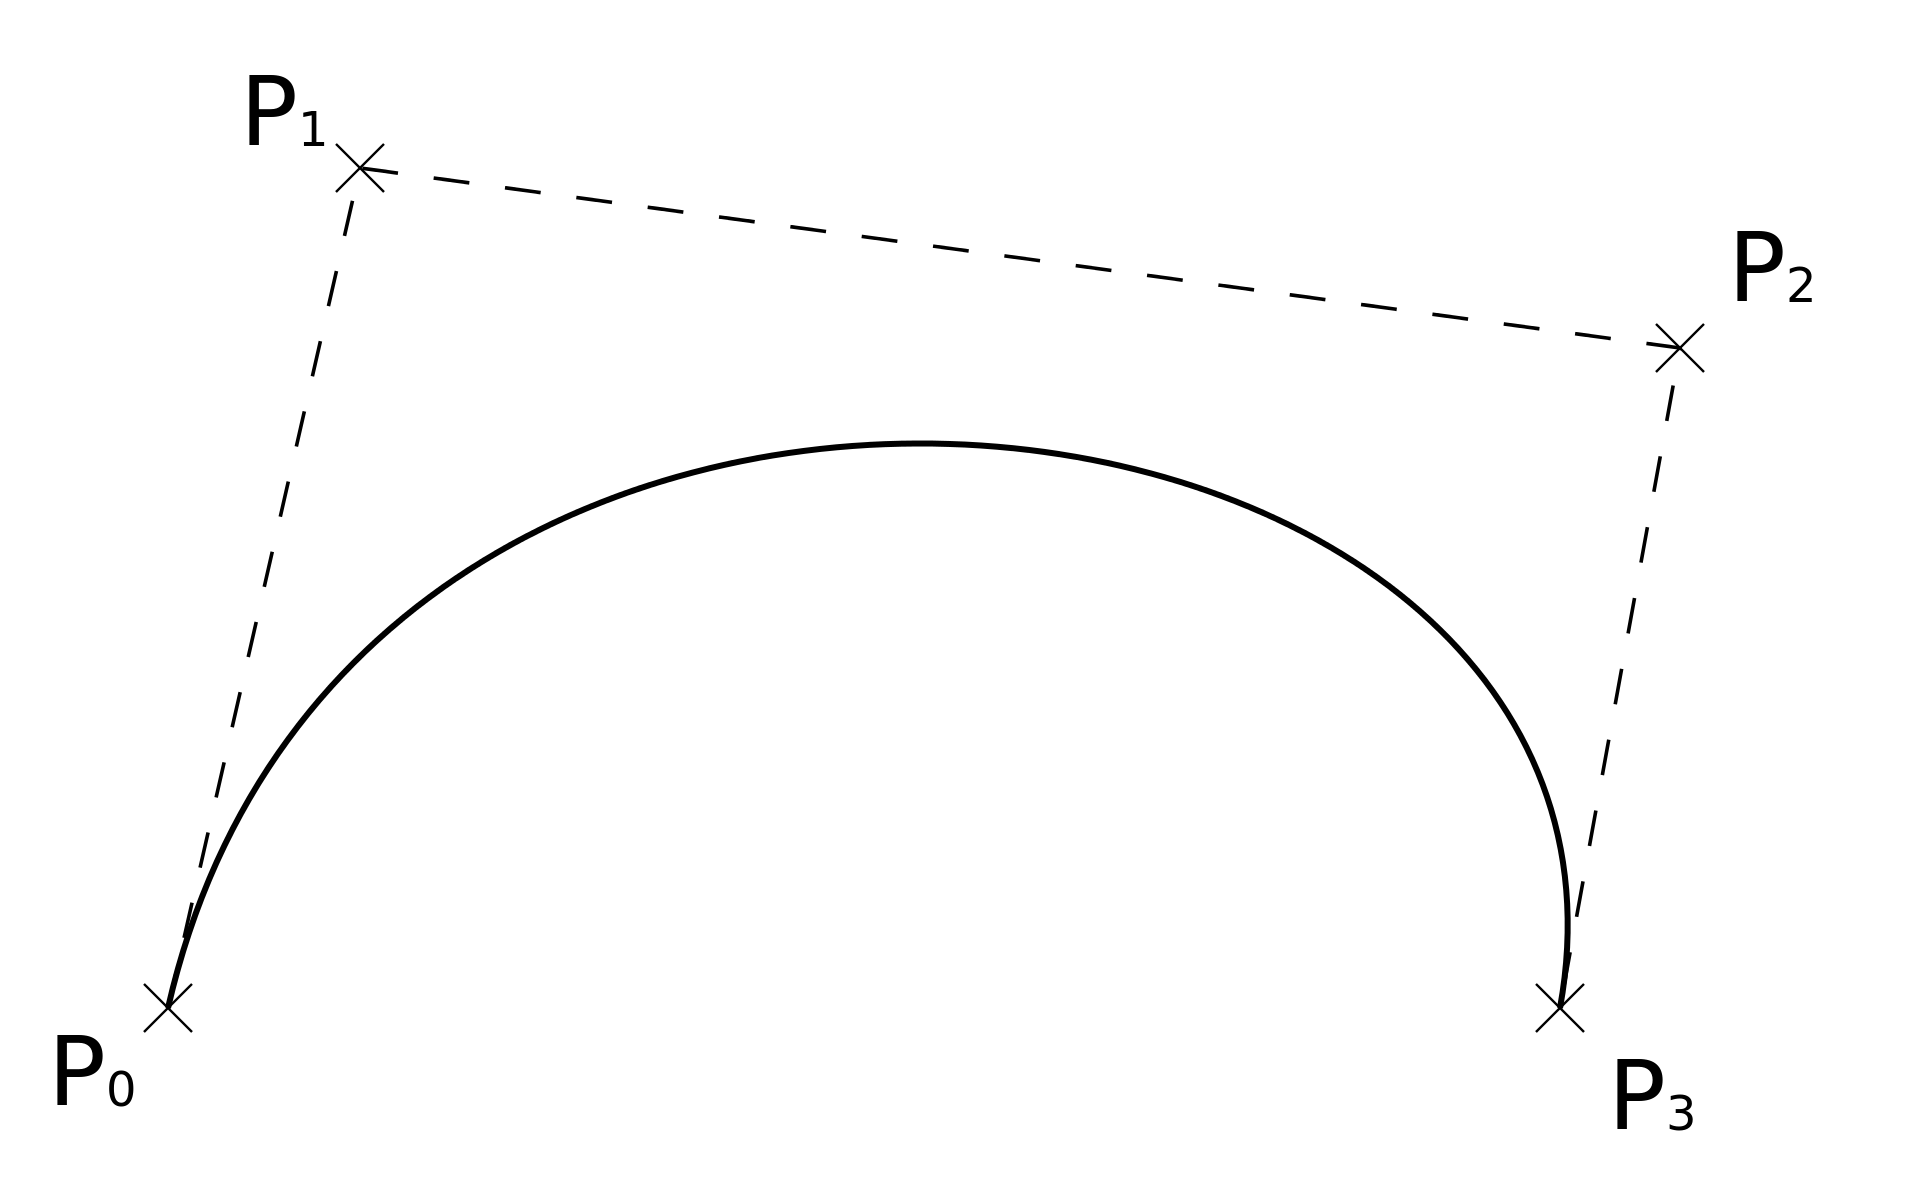
\includegraphics[width=0.5\linewidth]{fig/lit_rev/bezier_curve}
	\caption[Bezier curve.]{Bezier curve, courtesy of Wikipedia.}
	\label{fig:bezier_curve}
\end{figure}

\citet{jolly2009bezier} presented an approach to path planning for soccer robots based on Bezier curves. In robot soccer, it is important to hit the ball from the correct direction, making Bezier curves an appropriate choice. While the intended application of the approach is in robot soccer, the generation of the Bezier curves in itself is applicable for other scenarios as well. The approach is based on the selection of four control points, as shown in \figref{fig:bezier_soccer}. The first and last control points are taken as the estimated position of the robot and the target. The second control point is located based on the estimated heading of the robot and a distance ($d_1$ in the figure). Similarly, the third control point is located based on the desired final heading and a distance ($d_2$ in the figure). The distances to the second and third control points are determined through an iterative optimization algorithm which takes into account the acceleration limits of the robot.

\begin{figure}[h!]
	\centering
	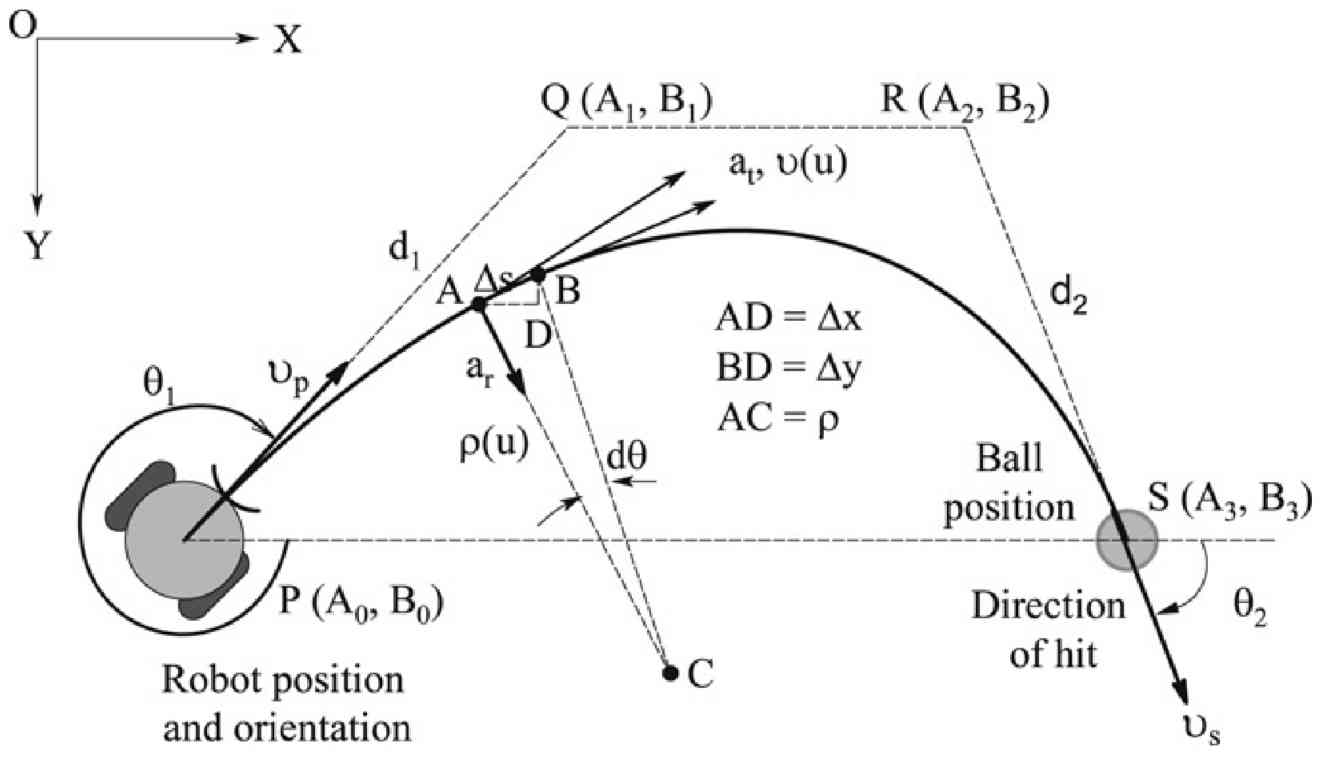
\includegraphics[width=0.5\linewidth]{fig/lit_rev/bezier_soccer.jpg}
	\caption[A Bezier curve ensuring that the robot hits the ball from the right direction in robot soccer.]{A Bezier curve ensuring that the robot hits the ball from the right direction in robot soccer \citep{jolly2009bezier}.}
	\vspace*{5.5in}
	\label{fig:bezier_soccer}
\end{figure}



\chapter{Problem formulation}

%IDEAL
This thesis considers the problem of autonomous USV maneuvering for complete bathymetric coverage of the seabed. The USV workspace is assumed to be a bounded rectangular 2D region, with possibly the presence of obstacles. The maneuvering system generates continuous steering control that allows the USV to \emph{efficiently} cover the seabed with its observation sensor, i.e. reducing undesired overlapping sensor coverage. Obstacles within the target region are avoided. The system operates with no prior knowledge of the target region.

%REALITY
Most existing complete coverage algorithms are offline and covers the target region using boustrophedon motions, and the spacing between the back-and-forth laps is determined by the coverage range of the robot's sensor or end-effector. However, when covering the seabed while navigating on the surface, the observation sensor's coverage range varies depending on the water depth. Consequently, existing complete coverage methods that are aimed towards land-based robots such as vacuum cleaners or lawnmowers with a constant coverage range, cannot directly be applied to USVs. There are works in the literature that consider varying coverage range due to water depth, for both ASVs and AUVs operating at constant depth. However, online approaches that also consider obstacles in the target region are still left largely unexplored.

%SOLUTION
The USV is assumed to be a Dubins vehicle, i.e. a non-holonomic vehicle that is constrained to move along planar paths of bounded curvature, and can only travel forward along the path. The observation sensor is a multibeam echosounder that covers the seabed in a swath directly beneath the USV and perpendicular to the moving direction. The swath extends a distance $c_p$ and $c_s$ in the port and starboard directions, respectively. A low-cost 2D lidar is mounted on top of the USV and used to detect and avoid obstacles on the surface. Moving obstacles can be considered as long as they move slowly compared to the USV. The system fuses information from lidar, IMU, and GNSS in order to maintain an always up-to-date map of obstacles in the surrounding environment. The map is partitioned into a grid, which is used by a path planning method to plan collision-free paths that ensure complete coverage of the seabed. These generated paths consist of a series of waypoints, and are further processed in order to generate feasible trajectories using simple Dubins paths. These trajectories take into account the turning radius, speed, and maximum stopping distance of the USV. Lastly, these trajectories are fed into a path following controller that generates continuous course and speed control that are passed to the Otter USV's onboard systems. A topology drawing of the control system and its information flow is shown in \figref{fig:topology}. Maritime Robotics' already existing systems, which need to be interfaced with, are marked in the figure.

\begin{figure}[h!]
	\centering
	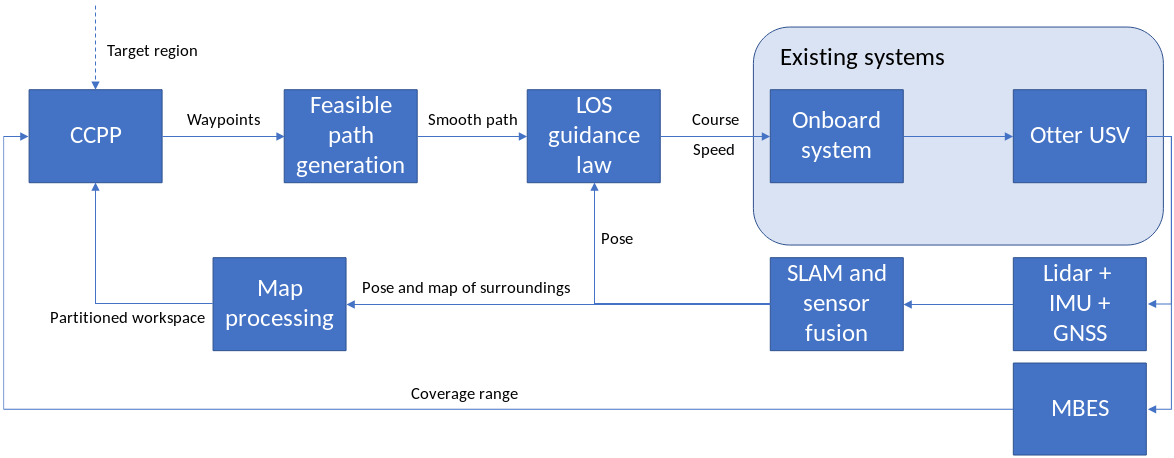
\includegraphics[width=1.0\linewidth]{fig/topology}
	\caption{The control system and its information flow.}
	\label{fig:topology}
\end{figure}

\chapter{Sensor fusion and SLAM} \label{ch:slam}

SLAM consists of simultaneous estimation of the state of a robot equipped with onboard sensors, and the construction of a map of the environment that the sensors are perceiving \citep{slamtut2006part1}. The robot state is often described by its pose (position and orientation), although other quantities may be included. The map represents aspects of interest (e.g. obstacles) describing the robot's surrounding environment. Both of these things, the robot pose and a map of the surroundings, are critical components for tasks such as path planning. Consequently, SLAM is often a key component in autonomous operations where a prior map of the environment is not available.

SLAM systems require some sort of mapping data about their surrounding environment. This data can come from sensors such as lidar \citep{cartographerPaper}, sonar \citep{norgren2018multibeam}, or camera \citep{orbslam2017} (often called visual SLAM or VSLAM). In order to increase reliability and robustness, most SLAM systems also support input from other types of sensors such as IMU, different types of odometry (e.g. wheel odometry for wheeled robots), altimeter for aerial vehicles, or GNSS \citep{website:Cartographer,hector2011slam}. As a result, SLAM is a valuable tool for sensor fusion. 

In this chapter, the sensors of the Otter USV are presented together with the drivers required to get the sensor data into ROS. The chapter also takes a closer look how the data from the sensors are used, and why the sensors are needed. Finally, the SLAM system Cartographer \citep{cartographerPaper} is set up for real-time 2D SLAM in ROS.

\section{Sensors and drivers}

\subsection{Lidar}

In this thesis, mapping of the surrounding environment is done with the RPLIDAR A3 \citep{website:rplidara3}, a low-cost 2D lidar. The lidar states a range of 25 m, 360-degree field of view, 16000 samples per second, and outdoor availability. A ready-to-use ROS driver, the \path{rplidar_ros} package \citep{website:rplidarDriver}, provides the system with \path{sensor_msgs/LaserScan} messages. This is a data type which holds an array of ranges and their corresponding angles for one complete revolution of the lidar. The lidar and a visualization of a laser scan is shown in \figref{fig:lidar_sensor}.

\begin{figure}[h!]
    \centering
	\makebox[\linewidth][c]{
	\begin{subfigure}[b]{0.5\textwidth}
		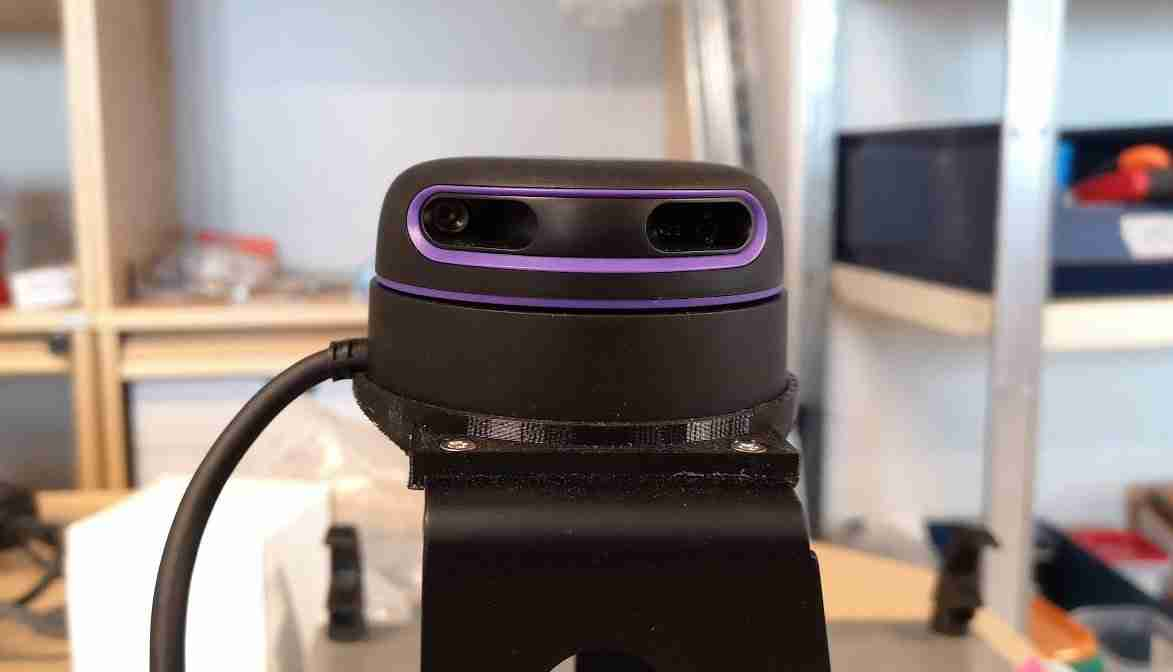
\includegraphics[width=1\linewidth]{fig/instrumentation/rplidara31}
		\caption{}
	\end{subfigure}
	\begin{subfigure}[b]{0.5\textwidth}
		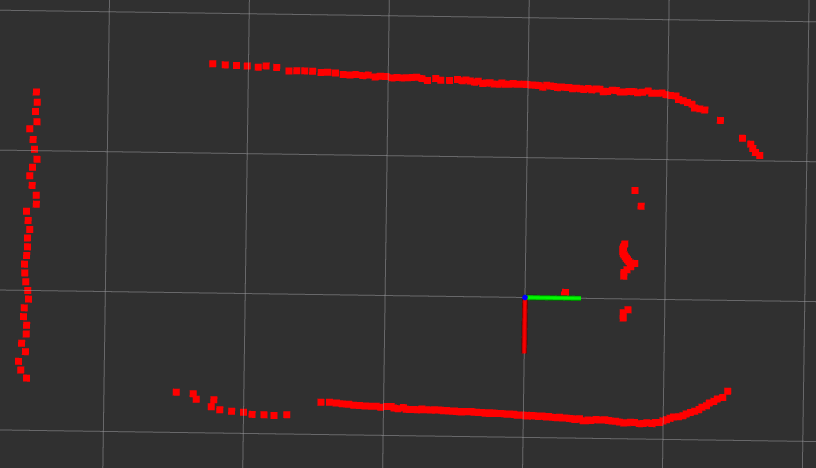
\includegraphics[width=1\linewidth]{fig/instrumentation/lidar_scan}
		\caption{}
	\end{subfigure}
	}
	\caption[The RPLIDAR A3]{(a) The RPLIDAR A3. (b) A lidar scan of a small room. The red, green and blue axis is the position of the lidar} \label{fig:lidar_sensor}
\end{figure}

It is possible to autonomously navigate a USV with only a lidar and SLAM, see for instance \citet{Ueland2016}. However, this requires a feature-rich environment in which it is always possible to find and recognize distinct features between subsequent lidar scans. Consequently, autonomous navigation with only a lidar is not feasible for situations where distances to the nearest obstacles often exceeds the range of the lidar. Additional sensors are also required in scenarios where the lidar is not able to see any difference in the environment between two consecutive poses, e.g. in a long corridor or while following a long uniform wall or edge. Since scenarios such as these are likely to be common in a typical application of the complete system, additional sensors are required.

\subsection{IMU}

Supplementing the lidar with an IMU increases the robustness and reliability of the sensing. This is because the IMU provides accurate orientation, rotational velocity, and linear acceleration, which can be used as initial estimates for the USV pose when comparing subsequent lidar scans in SLAM. This is especially useful for a USV operating on the water surface, since roll and pitch motions are otherwise hard to compensate for. The implemented system uses an AHRS of the type Xsens MTi \citep{website:xsens}, see \figref{fig:xsens}. The Xsens MTi comes with a ROS driver, the \path{xsens_driver} package \citep{website:xsensDriver}. This driver provides ROS with \path{sensor_msgs/Imu} messages, which contain orientation, angular velocity, and linear acceleration. The Xsens, being an AHRS, reports orientation relative to magnetic north, and the magnetic declination of the operating area can be looked up (e.g. at \citet{website:magcalc}). Having the orientation relative to true north makes it possible to later combine the IMU data with for example GNSS data.

%Thus, true heading is available to the system and can be used to translate angles in the SLAM map to course angle assignments.

\begin{figure}[h!]
	\centering
	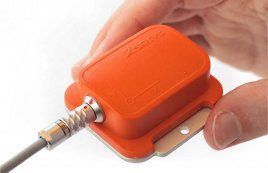
\includegraphics[width=0.5\linewidth]{fig/instrumentation/xsens_mti2}
	\caption[The Xsens MTi.]{The Xsens MTi AHRS, courtesy of Xsens.}
	\label{fig:xsens}
\end{figure}

\subsection{GNSS}

The combination of lidar and IMU works very well in many situations. SLAM systems usually have no problem localizing and generating maps when there are many objects within the range of the lidar. However, consider scenarios such as in \figref{fig:lidar_gnss} where the lidar detects nothing at all or too little for accurate localization. Based only on the detections generated from \figref{fig:lidar_gnss}b, the USV can be at any point along the wall. In situations such as these, the SLAM system is mostly relying on IMU data for positioning, and position estimates based on integration of linear accelerations from an IMU will quickly drift. For the intended purposes of the implemented system, scenarios such as these are to be expected. Thus, another form of positioning is needed, and in this case GNSS is used.

\begin{figure}[h!]
    \centering
	\makebox[\linewidth][c]{
	\begin{subfigure}[b]{0.5\textwidth}
		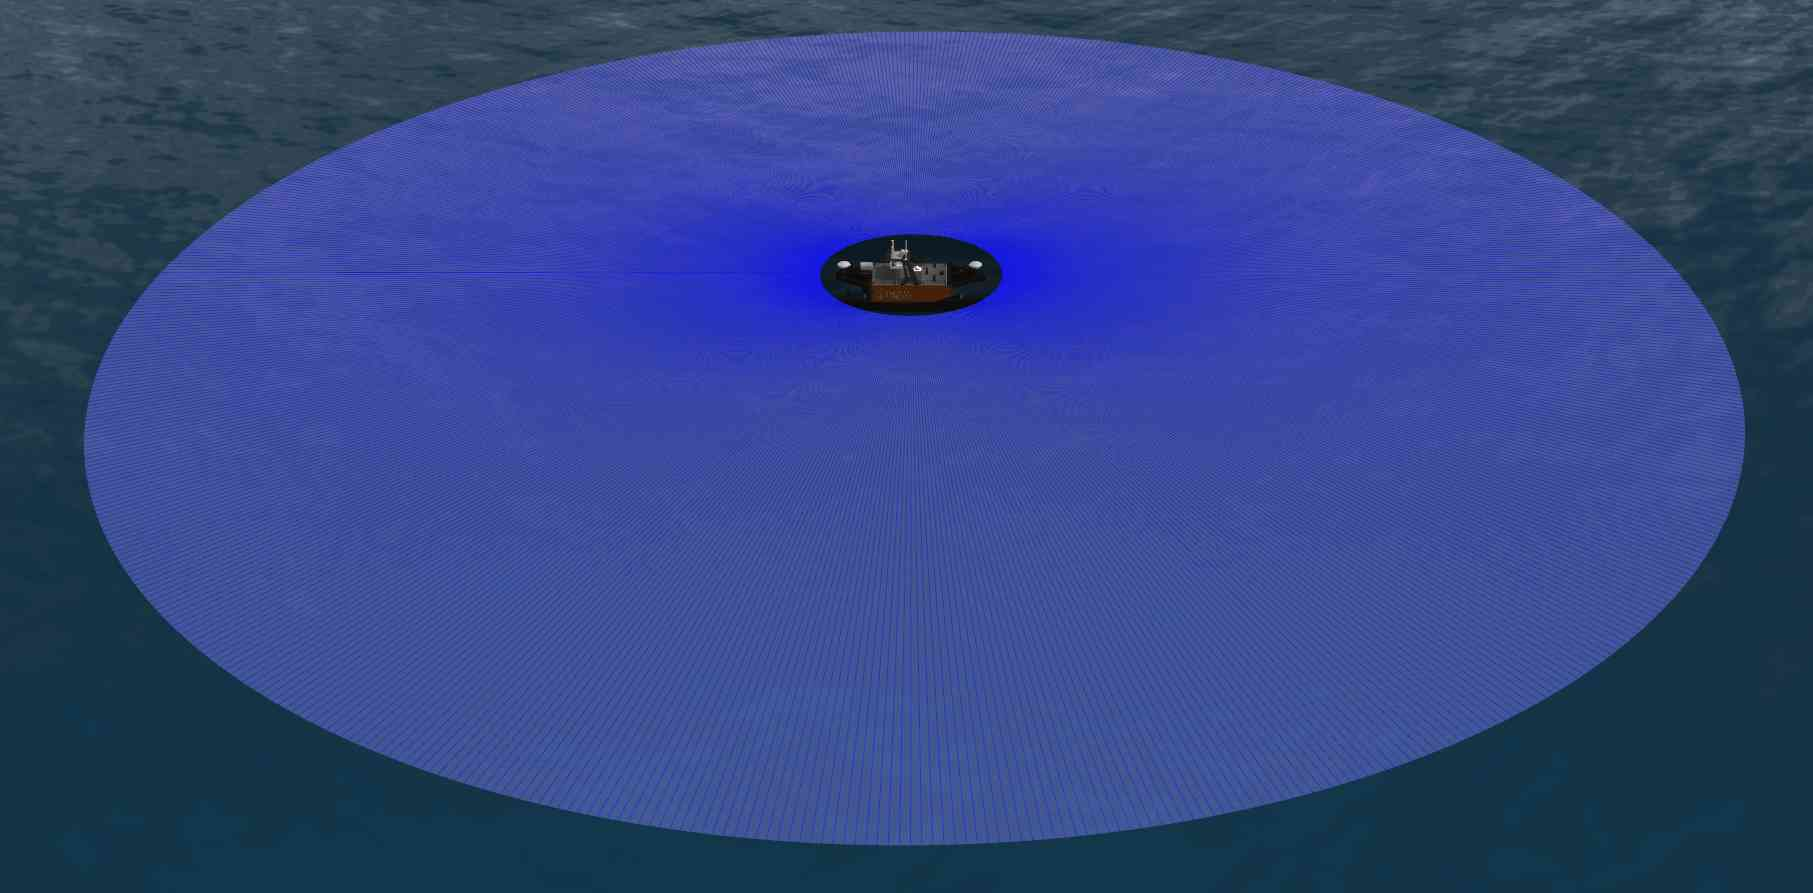
\includegraphics[width=1\linewidth]{fig/instrumentation/lidar_nothing.jpg}
		\caption{}
	\end{subfigure}
	\begin{subfigure}[b]{0.5\textwidth}
		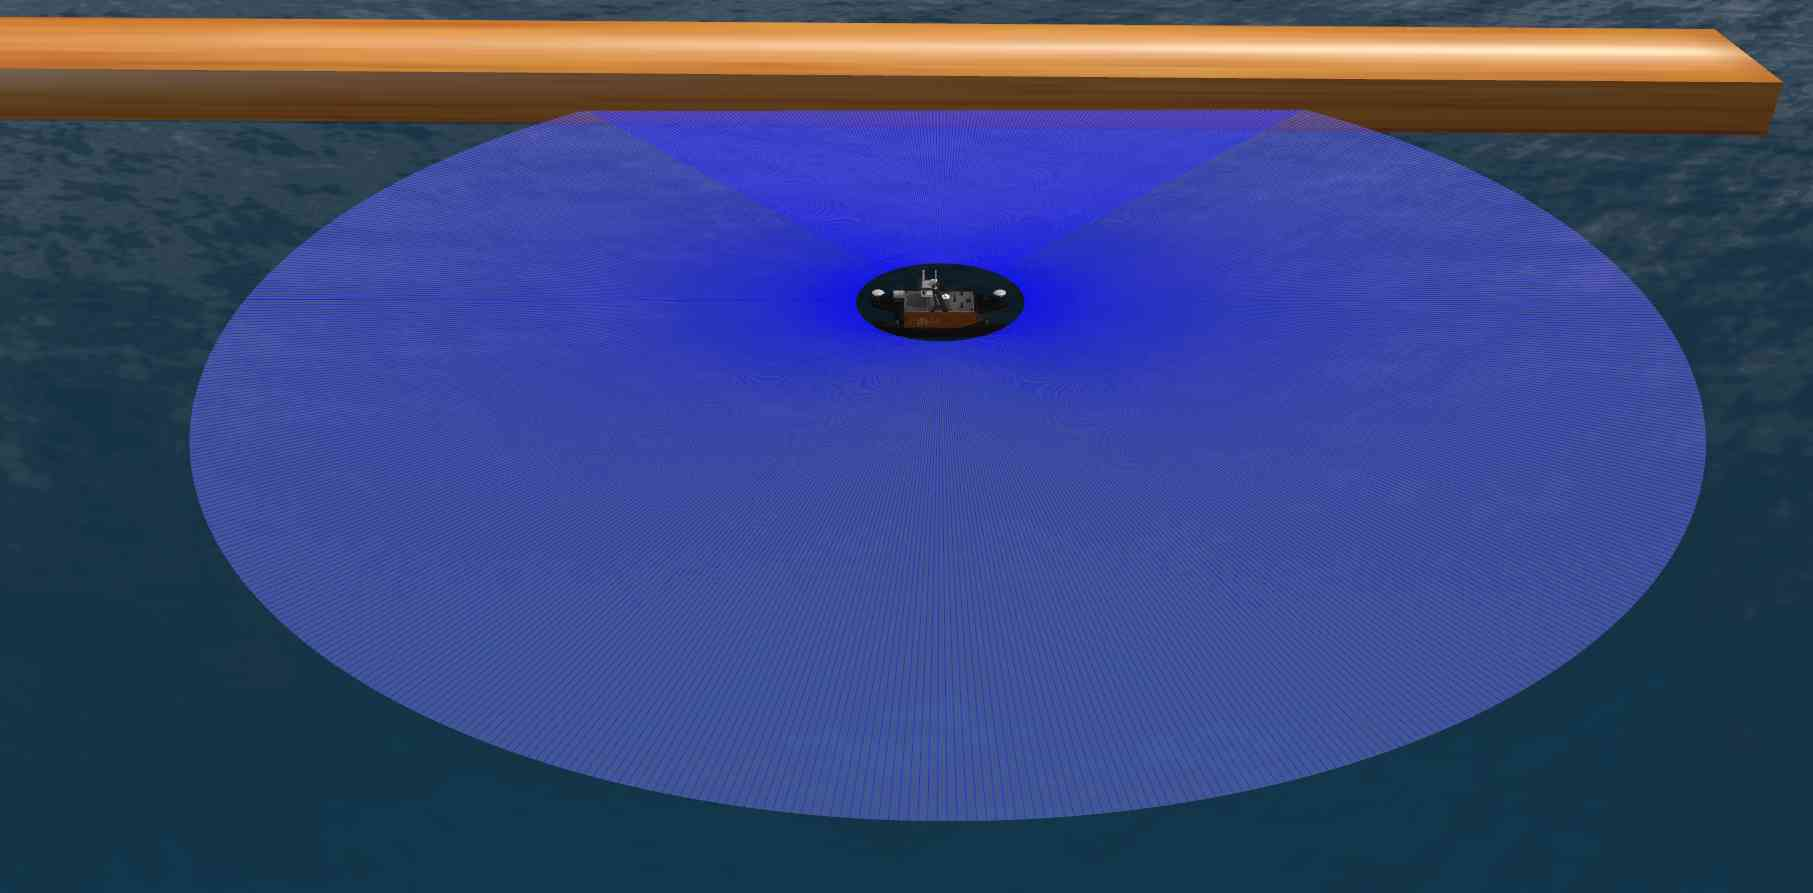
\includegraphics[width=1\linewidth]{fig/instrumentation/lidar_only_wall.jpg}
		\caption{}
	\end{subfigure}
	}
	\caption[Lidar detects nothing or too little for accurate localization.]{(a) No obstacles are within the lidar range. (b) The section of the wall within the lidar range does not provide enough information for localization.} \label{fig:lidar_gnss}
\end{figure}

The GNSS receiver on the USV reports its position as NMEA 0183 GGA messages. NMEA 0183 is a data specification standard for communication between marine electronics, defined by the National Marine Electronics Association \citep{wiki:nmea}. The GGA messages contain, most importantly, the latitude and longitude of the GNSS receiver. These messages are parsed with the \path{nmea_navsat_driver} ROS driver \citep{website:nmeaDriver}, which has been slightly modified to allow incoming NMEA messages over TCP. The driver provides the system with \path{sensor_msgs/NavSatFix} messages, which contain the latitude and longitude.

% The driver also provides the course angle $\chi$ as \code{geometry\_msgs/QuaternionStamped}.

\subsection{MBES}

The multibeam echosounder measures the depth in a fan shape beneath the USV. This data is not necessary for collision-free maneuvering on the surface, and is therefore not included in SLAM. There are SLAM systems that use MBES data (e.g. \citet{norgren2018multibeam}), so the MBES could potentially be included in SLAM in order to increase the accuracy. In this thesis, however, the MBES is only used for keeping track of the covered area and adapting the spacing between laps in the boustrophedon motions CCPP method. 

To use the MBES, the coverage range must be calculated. Let a detection point be described by the angle $\alpha$ relative to a line straight down from the USV, and let the reported distance for that angle be $f(\alpha)$, see \figref{fig:mbes_range}. Finding the detection point with the maximum angle $\alpha_{max}$ and minimum angle $\alpha_{min}$, it is then possible to find the coverage range in the port and starboard direction with
\begin{align}
c_p &= f(\alpha_{min}) \sin(\alpha_{min}) \\
c_s &= f(\alpha_{max}) \sin(\alpha_{max})
\end{align}
where $c_p$ and $c_s$ are the coverage ranges in port and starboard directions.

\begin{figure}[h!]
	\centering
	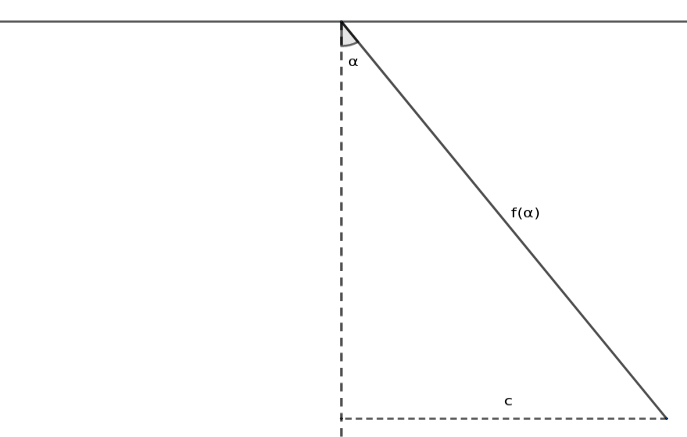
\includegraphics[width=0.5\linewidth]{fig/instrumentation/mbes_range2}
	\caption{Geometry of detection points of the MBES.}
	\label{fig:mbes_range}
\end{figure}

\section{SLAM with Cartographer}

Cartographer provides real-time SLAM in 2D and 3D across multiple platforms and sensor configurations \citep{website:Cartographer}. In this thesis, the ROS integration of Cartographer \citep{website:CartographerRos} is applied for 2D operation. By using the 2D version of Cartographer it is assumed that the floor (water surface) is flat, which is an okay assumption with a 2D lidar in sheltered waters. This only causes trouble if the heave motion of the USV causes the lidar to detect different things at different heights. The 2D version is chosen mainly because it is simpler to work with, as it requires fewer parameters to be tuned. Furthermore, the additional benefits of a 3D map are not required for the application in this thesis.

Out of the box, Cartographer accepts \path{sensor_msgs/LaserScan} and \path{sensor_msgs/Imu} messages from the lidar and IMU. However, the 2D version does not readily accept \path{sensor_msgs/NavSatFix} messages from the GNSS receiver. To get around this, it is possible to fuse data from the IMU and GNSS with an extended Kalman filter (EKF) in order to generate pose estimates as \path{nav_msgs/Odometry} messages. These messages can in turn be provided to Cartographer. The \path{robot_localization} package in ROS \citep{ros:robotlocalization} offers a collection of state estimation implementations for incorporation of GNSS data which has been used in this thesis. The information flow described in this chapter is illustrated in \figref{fig:sensor_fusion}.

\begin{figure}[h!]
	\centering
	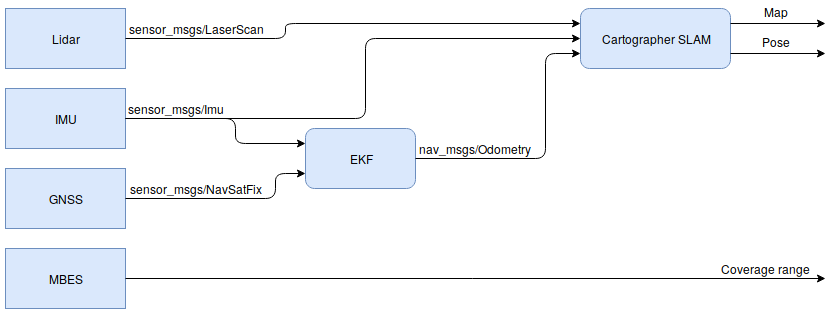
\includegraphics[width=1.0\linewidth]{fig/instrumentation/sensor_fusion}
	\caption{Information flow in sensor fusion and SLAM.}
	\label{fig:sensor_fusion}
\end{figure} 

Tuning Cartographer is difficult, as it is a very complex system where many of the parameters affect each other. A tuning methodology is provided by the authors at \citet{website:CartographerRos}. Tuning includes, among many other things, to set parameters for the scan matcher, the size and resolution of the submaps, and how much to trust odometry. For instance, since the provided odometry is a fusing of accurate IMU and GNSS data, it should be trusted with a high weight. The exact values to set is often a matter of experimenting and seeing what yields the best results. The parameters used in the experiments are provided in Appendix \ref{app:cartographer}.



\chapter{Map processing and workspace partitioning} \label{ch:partition}

The sensor fusion and SLAM subsystem described in Chapter \ref{ch:slam}, provides the rest of system with a map of the surrounding environment and the pose of the USV. The SLAM map in its raw form, however, is often not a suitable workspace representation for many CCPP methods. The strategy used for representing the operational workspace largely determines what kind of path planning methods that can be used. That is why workspace partitioning is such an important part of CCPP. This chapter describes two different partitioning methods, each of which will be used in a different CCPP method. However, the partitioning methods do not operate on the raw SLAM map either, some map processing is applied first.

\section{Map processing and rolling window} \label{sec:map_processing}

Information about the surrounding environment is only gathered by the lidar, meaning the only new information in the SLAM map is contained within the lidar range. There is one exception to this, and that is corrections to the SLAM map caused by loop closures. However, these corrections are often small and are not relevant for the generation of new waypoints in the immediate vicinity of the USV. Therefore, a huge increase in computational efficiency can be gained by only considering changes to the map within the lidar range. In order to do this, a rolling window is applied. The rolling window is a 2D square occupancy grid which inscribes the circle that is the lidar's coverage around the USV, and is always centered at the USV's position. The rolling window is shown in \figref{fig:costmap}.

In the occupancy grid, each cell has an associated probability $[0, 100]$ that determines whether it is an obstacle or free space. Unknown is $-1$. The following categorization is applied in this thesis
\begin{equation}
\text{Cell status} = 
\begin{cases}
\text{unknown}, & \text{if cell value} = -1 \\ 
\text{obstacle}, & \text{if cell value} \geq 50 \\
\text{free}, & \text{otherwise.}
\end{cases}
\end{equation}
In order to accurately represent the environment with an occupancy grid, the resolution of the grid must be high. However, a higher resolution also increases requirements to processing power. Thus, $\SI{20}{cm}$ per cell is chosen as the resolution, which is the same as the resolution of the SLAM map. 

\begin{figure}[h!]
	\centering
	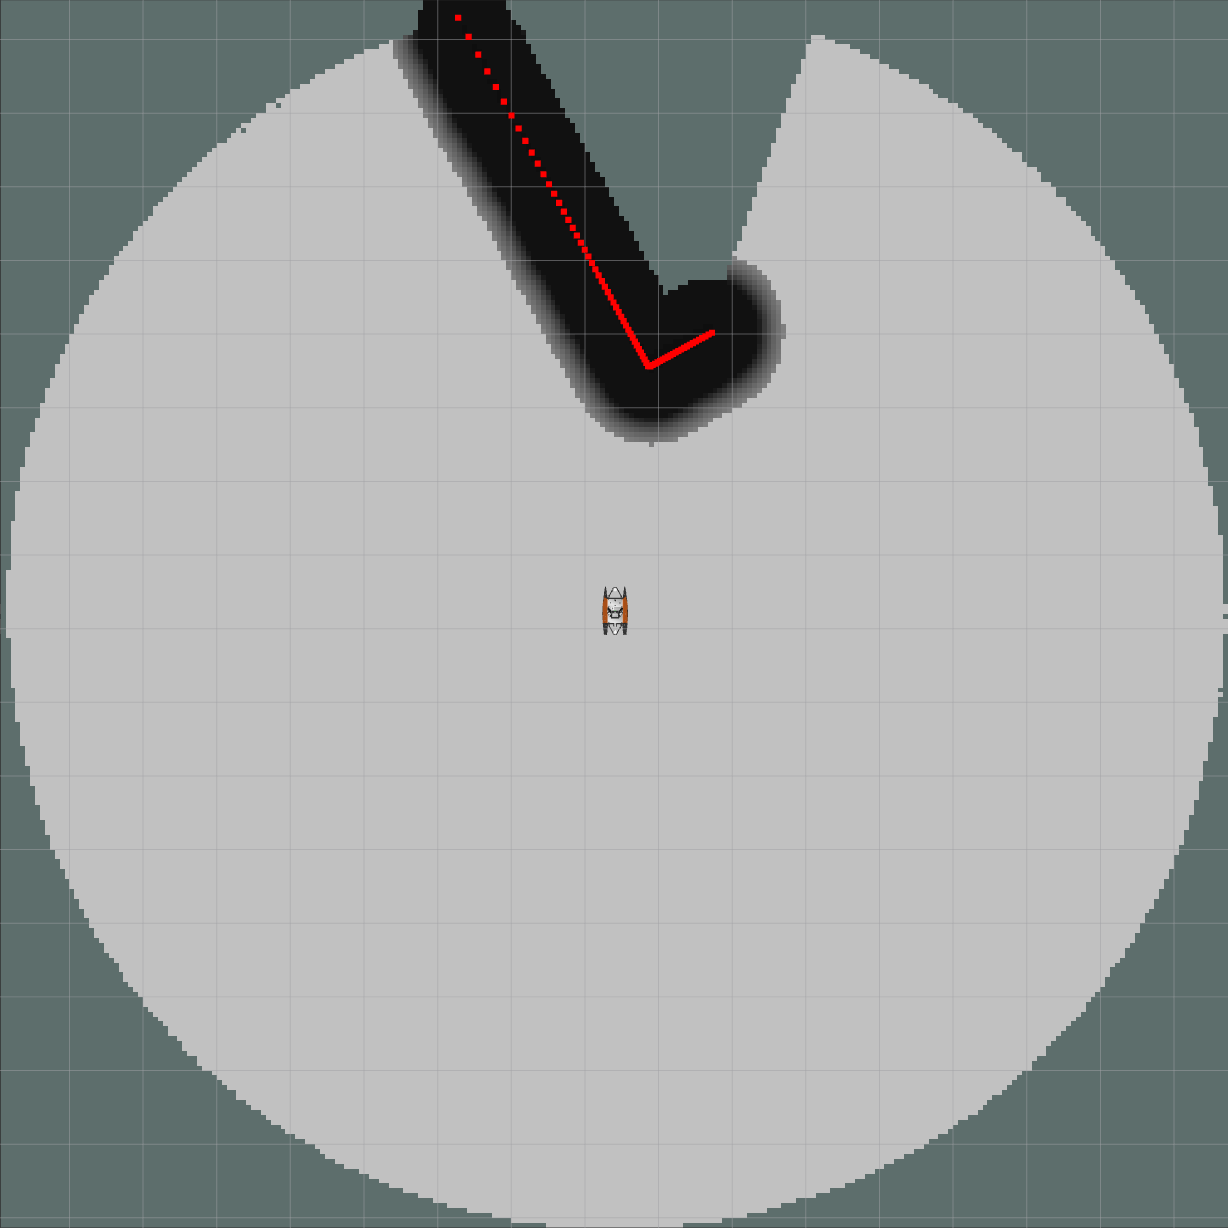
\includegraphics[width=0.5\textwidth]{fig/partition/costmap}
	\caption[Rolling window occupancy grid around the USV.]{Rolling window occupancy grid around the USV. The red dots are lidar detections, gray cells are free space, black cells are inflated obstacles, and the rest is unknown.}
	\label{fig:costmap}
\end{figure}

The USV is in collision with an obstacle whenever some part of the USV is located at a cell that is an obstacle. Thus, no collision can occur when the closest obstacle is located more than a distance $r_{max}$ away, where $r_{max}$ is the radius of a circle circumscribing the USV's footprint. To account for the USV's footprint, obstacles must therefore be inflated with an inflation radius $r_i > r_{max}$. Increasing the inflation radius further creates a buffer safety zone around obstacles. Obstacle inflation means that any cell $(x,y)$ is considered an obstacle if the distance to any obstacle $(x_{obs},y_{obs})$ is shorter than the inflation radius. In the implemented system, the inflation radius is chosen as $r_i = \SI{5.0}{\meter}$ while the maximum footprint is $r_{max} = \SI{1.0}{\meter}$ for the Otter USV. This ensures that the USV does not travel to close to other boats, and allows for operator intervention in case something goes wrong. The obstacles of \figref{fig:costmap} are inflated.

The rolling window is implemented with the \path{costmap_2d} package from the ROS \path{navigation} stack \citep{marder2010office}. The rolling window is published as a \path{nav_msgs/OccupancyGrid} message in ROS at frequent intervals.


\section{Circular cell partitioning} \label{sec:circle_partition}

\citet{guo2004coverage} considered the problem of covering a rectangle using a minimum number of circles. Their motivation for partitioning the workspace into circles comes from the fact that the coverage range of their robot is represented by a circle. The coverage of the MBES sensor used in this thesis, however, is a swath on the seabed perpendicular to the USV's moving direction. Nevertheless, the use of circles to represent the covered area is still a valid approach. Consider, without loss of generality, that the USV travels through the center of each circle with a non-negative speed. With the added assumption that the radius of the circles is smaller than the MBES sensor's coverage in both port and starboard direction. This ensures that by reaching the circle's center, at least half of the circle is covered. When leaving the circle, the remaining half is guaranteed to be covered.

An important thing to note, is that the coverage range of the MBES varies depending on the water depth. To ensure complete coverage, it is therefore necessary to use a cell size determined by the shallowest point in the target region. This will result in undesired overlapping coverage if the coverage range varies a lot.

%\todo[inline]{Mention that the approach is not effective with hugely varying swath widths? Save to discussion}
% One disadvantage with this approach, is that the sensor’s field of view varies depending on the depth of the water. To ensure complete coverage, it is therefore necessary to use a cell size determined by the shallowest point on the target surface, resulting in undesired coverage overlapping among the cells.

Consider the rectangular area $\bm{W}$, where $x_w$ and $y_w$ are the lengths of the rectangular edges along the x-axis and y-axis, respectively. Circles of radius $r_c$ are placed in strips parallel to the y-axis, such that the distance between the centers of any two adjacent circles is $\sqrt{3}r_c$. $m$ columns of these strips are placed such that the distance between any two adjacent strips is $\frac{3}{2}r_c$. The layout of the circles can be seen in \figref{fig:circular_partition}.

\begin{figure}[h!]
	\centering
	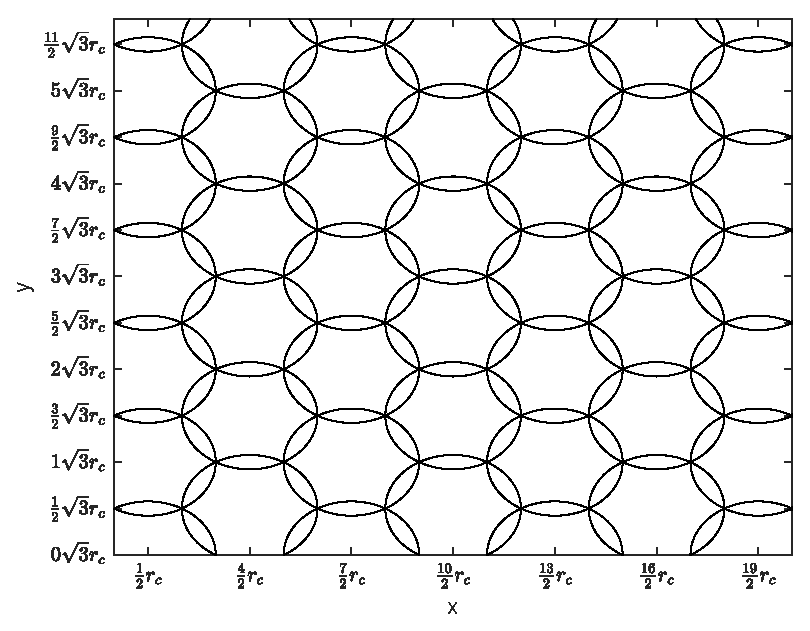
\includegraphics[width=0.5\textwidth]{fig/ccpp/circular_partition}
	\caption{Covering a rectangle using a minimum number of disks.}
	\label{fig:circular_partition}
\end{figure}

In a global cartesian coordinate system with the origin in the bottom left corner, $m$ columns of these strips are placed, each containing $n_l$ circles. The number of columns $m$ is determined by
\begin{equation} \label{eq:circle_partition_m}
m =
\begin{cases}
\floor*{ \frac{x_w}{\frac{3}{2}r_c} } + 1, & \text{if } \frac{x_w}{\frac{3}{2}r_c} \Mod{1} \leq \frac{2}{3} \\
\\
\floor*{ \frac{x_w}{\frac{3}{2}r_c} } + 2, & \text{if } \frac{x_w}{\frac{3}{2}r_c} \Mod{1} > \frac{2}{3}, \\
\end{cases}
\end{equation}
and the number of circles $n_l$ in a column is determined by
\begin{equation} \label{eq:circle_partition_nl}
n_l =
\begin{cases}
\floor*{ \frac{y_w}{\sqrt{3}r_c} } + 1, & \text{if } \frac{y_w}{\sqrt{3}r_c} \Mod{1} \leq \frac{1}{2} \\
\\
\floor*{ \frac{y_w}{\sqrt{3}r_c} } + 1 + (l \Mod{2}), & \text{if } \frac{y_w}{\sqrt{3}r_c} \Mod{1} > \frac{1}{2}. \\
\end{cases}
\end{equation}
$\floor*{x}$ is the floor function and mod is the modulo function. The center coordinates of a circle located at column $1 \leq l \leq m$ and row $1 \leq k \leq n_l$ are given by
\begin{equation} \label{eq:circle_partition_center}
[x_c^{kl}, y_c^{kl}] =
\begin{cases}
\left[ \left( \frac{3}{2}l - 1 \right)r_c, (k - 1)\sqrt{3}r_c \right], & \text{if } l \Mod{2} = 1 \\
\\
\left[ \left( \frac{3}{2}l - 1 \right)r_c, \left(k - \frac{1}{2}\right)\sqrt{3}r_c \right], & \text{if } l \Mod{2} = 0
\end{cases} 
\end{equation}

Equations \eqref{eq:circle_partition_m}, \eqref{eq:circle_partition_nl}, and \eqref{eq:circle_partition_center} have small corrections to those presented by \citet{guo2004coverage}. However, the proof of minimum number of circles still remains valid with these corrections \citep{Scibilia2012}.

A flag $f(r,c)$ is defined for a cell at row $r$ and column $c$ in the grid to indicate its status as either unknown, free, or obstacle
\begin{equation} \label{eq:circular_cell_status}
f(r,c) = 
\begin{cases}
0, & \text{if it is unknown} \\
1, & \text{if it is free} \\
2, & \text{if it is obstacle.} 
\end{cases}
\end{equation}
The status of the cells are updated based on data from the rolling window in Section \ref{sec:map_processing}. The circles have a radius $r_c$ which is a lot bigger than the size of the cells in the rolling window. Thus, a circle is considered blocked if any of the cells from the rolling window representing the same area are blocked. If all cells are free, the circle is considered free. Else, the circle is considered unknown. In addition, each circle also has a flag setting it as either covered or uncovered depending on if the USV has traveled through the center of the circle. \figref{fig:circle_partition} shows how the processed SLAM map is partitioned.

\begin{figure}[h!]
    \centering
	\makebox[\linewidth][c]{
	\begin{subfigure}[b]{0.5\textwidth}
		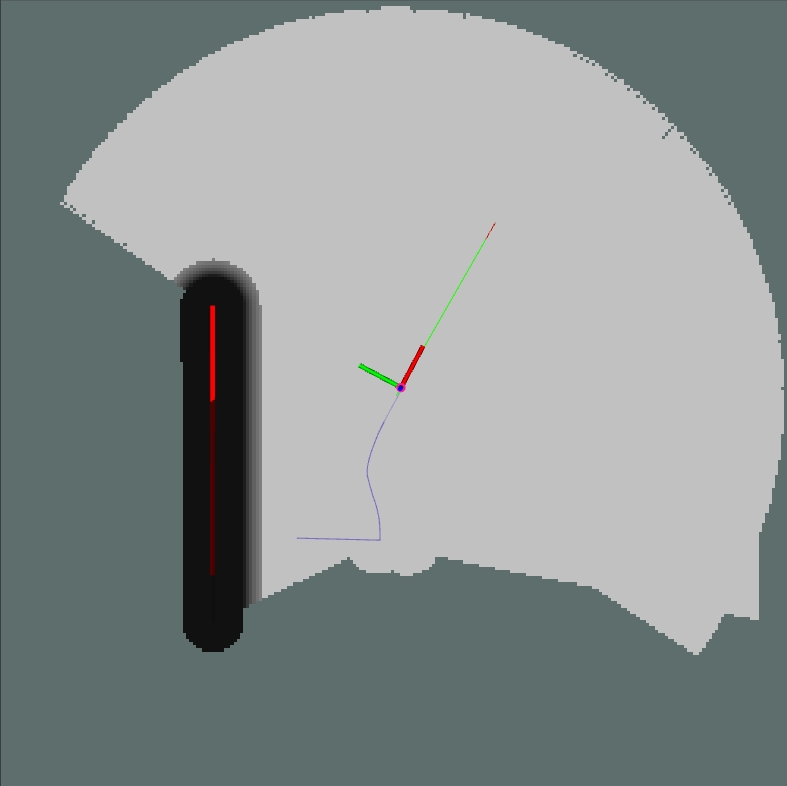
\includegraphics[width=1\linewidth]{fig/partition/circle1}
		\caption{}
	\end{subfigure}
	\begin{subfigure}[b]{0.5\textwidth}
		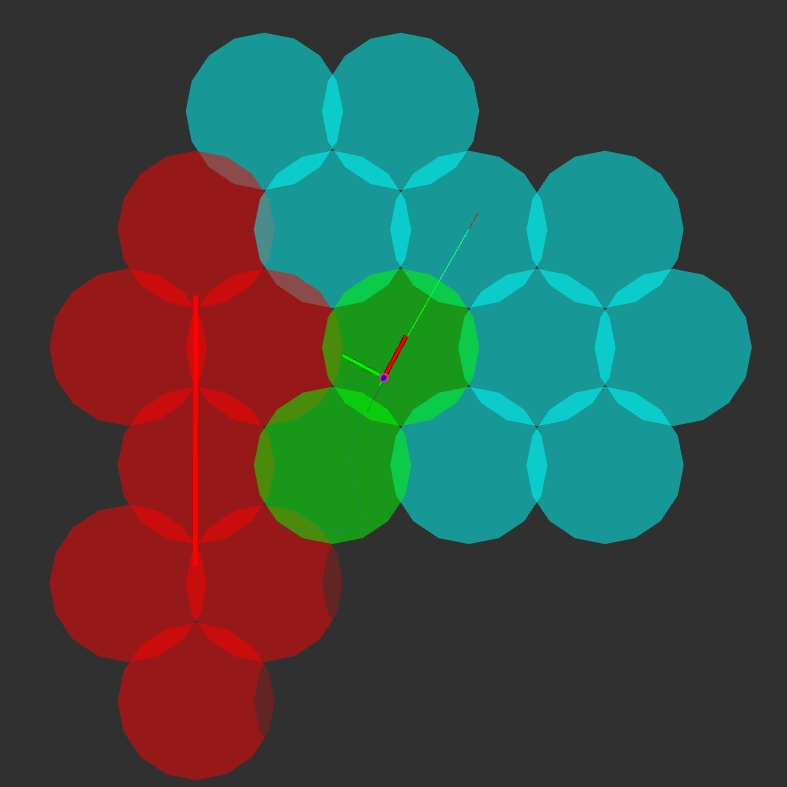
\includegraphics[width=1\linewidth]{fig/partition/circle2}
		\caption{}
	\end{subfigure}
	}
	\caption[Circular cell partitioning.]{Circular cell partitioning. (a) Processed SLAM map. The red dots are lidar detections, gray cells are free space, black cells are inflated obstacles and the rest is unknown. (b) The processed map partitioned into circular cells. Red circles represent obstacles, green circles represent covered free space, blue circles represent uncovered free space, and the rest is unknown.} \label{fig:circle_partition}
\end{figure}

\FloatBarrier

\section{Square cell partitioning} \label{sec:square_partition}

%\todo[inline]{Write this after finished implementing and testing.}

A grid-based map representation is proposed in which the entire workspace is partitioned into square cells of equal size $e_{cell}$. The grid map works partly as an occupancy grid, where each cell contains occupancy information to indicate its status as either free space, obstacle, or unknown
\begin{equation} \label{eq:square_cell_status}
f(r,c) = 
\begin{cases}
0, & \text{if it is unknown} \\
1, & \text{if it is free} \\
2, & \text{if it is obstacle} 
\end{cases}
\end{equation}
where $f(r,c)$ is a flag that takes the row $r$ and column $c$ as arguments, and returns the status of the cell. In addition, each cell has a flag indicating if the cell has been covered. As the USV moves around in the workspace, data from the rolling window of Section \ref{sec:map_processing} is used to update the status of the cells. The size of the cells in the grid map is larger than the size of the cells in the rolling window. This means a cell in the grid map is only considered free if all of the cells in the rolling window representing the same area are also free. If some of them are obstacles, the cell is set as an obstacle. Otherwise, the status is unknown. \figref{fig:square_partition} shows how the processed SLAM map is partitioned.

\begin{figure}[h!]
    \centering
	\makebox[\linewidth][c]{
	\begin{subfigure}[b]{0.5\textwidth}
		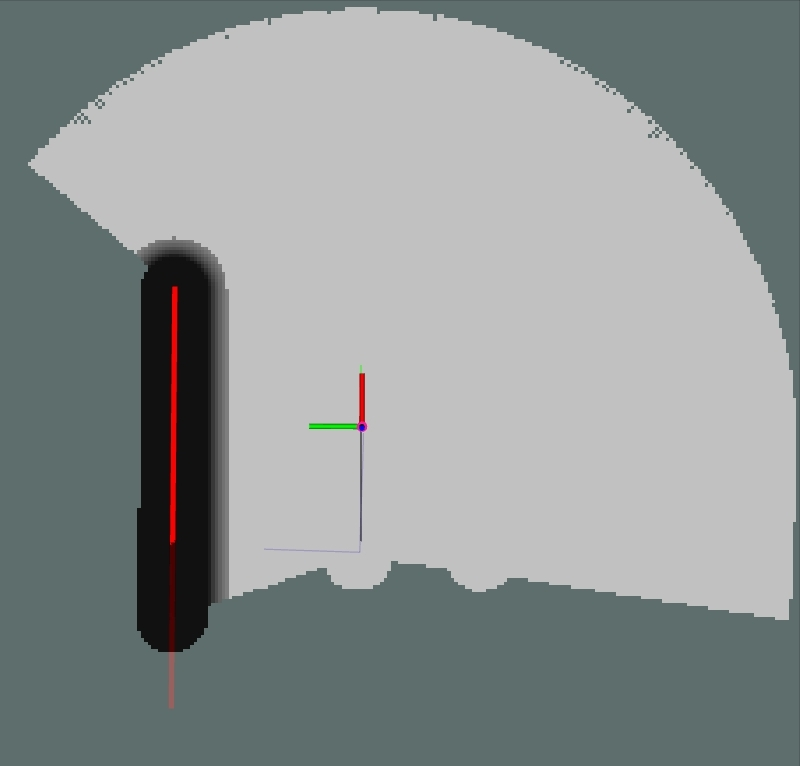
\includegraphics[width=1\linewidth]{fig/partition/square1}
		\caption{}
	\end{subfigure}
	\begin{subfigure}[b]{0.5\textwidth}
		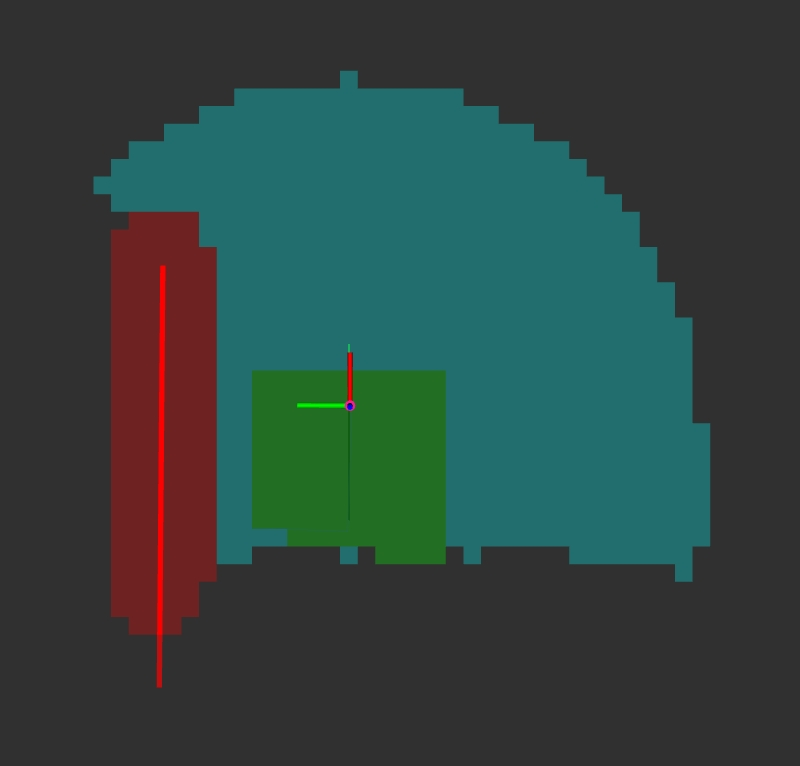
\includegraphics[width=1\linewidth]{fig/partition/square2}
		\caption{}
	\end{subfigure}
	}
	\caption[Square cell partitioning.]{Square cell partitioning. (a) Processed SLAM map. The red dots are lidar detections, gray cells are free space, black cells are inflated obstacles and the rest is unknown. (b) The processed map partitioned into square cells. Red squares represent obstacles, green squares represent covered free space, blue squares represent uncovered free space, and the rest is unknown.} \label{fig:square_partition}
\end{figure}

Consider the rectangular area $\bm{W}$, where $x_w$ and $y_w$ are the lengths of the rectangular edges along the x-axis and y-axis, respectively. The number of columns $m$ is determined by
\begin{equation}
m = \ceil*{\frac{x_w}{e_{cell}}}
\end{equation}
and the number of rows $n$ is
\begin{equation}
n = \ceil*{\frac{y_w}{e_{cell}}}.
\end{equation}
The center coordinates of a cell located at column $1 \leq l \leq m$ and row $1 \leq k \leq n$ are given by
\begin{equation}
\left[x_c^{kl},y_c^{kl}\right] = \left[\left(l - \frac{1}{2}\right) e_{cell}, \left(k - \frac{1}{2}\right) e_{cell}\right].
\end{equation}
Consequently, the row and column of a cell containing the point $(x,y)$ are given by
\begin{equation}
[l,k] = \left[\floor*{\frac{x}{e_{cell}}} + 1, \floor*{\frac{y}{e_{cell}}} + 1 \right].
\end{equation}

\subsection{Representing the varying coverage range of the MBES} \label{sec:handle-mbes}

The coverage of the MBES sensor is a swath of variable length on the seabed perpendicular to the USV's moving direction. Let the $(x,y)$ and $\psi$ be the position and heading of the USV in the grid map (z-axis downward), and let $c_{s}$ and $c_{p}$ be the swath length in starboard and port direction, respectively. The cells covered by the swath can then be determined. First, a line segment is constructed between the endpoints of the swath
\begin{equation}
\left[ x + c_{s} \cdot \cos(\psi + \frac{\pi}{2}), y + c_{s} \cdot \sin(\psi + \frac{\pi}{2}) \right]
\end{equation}
and
\begin{equation}
\left[ x + c_{p} \cdot \cos(\psi - \frac{\pi}{2}), y + c_{p} \cdot \sin(\psi - \frac{\pi}{2}) \right].
\end{equation}
A modified version of the Bresenham's line algorithm \citep{wiki:bresenham} is then used to find the cells that are covered by this line segment. The modified algorithm by \citet{supercoverAlgo} finds the supercover line, i.e. all the points intersected by a line between two endpoints. This is an algorithm often used in computer graphics for selecting which pixels to set when drawing a line. In this case, it is instead used to select which cells to set as covered. An illustration is shown in \figref{fig:cover_line}.

\begin{figure}[h!]
    \centering
	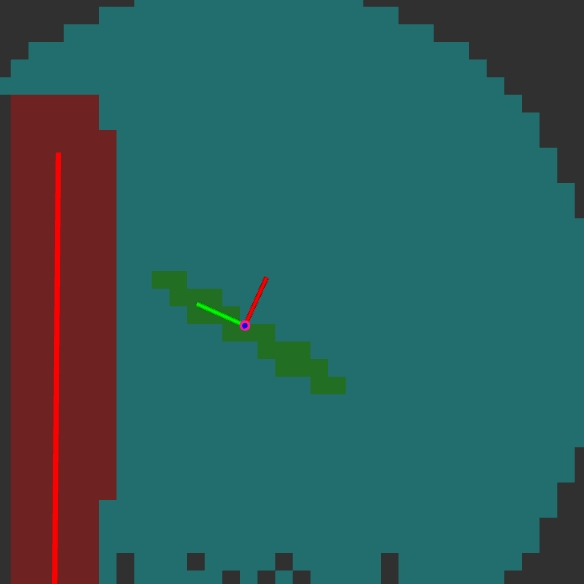
\includegraphics[width=0.5\linewidth]{fig/partition/cover_line}
	\caption{The square cell partition uses the coverage range of the MBES to determine which cells are set as covered. } \label{fig:cover_line}
\end{figure}

The method of representing the varying coverage range described above, is an approximate method. A small cell size $e_{cell}$ results in a more accurate representation of the covered area. On the other hand, a larger cell size reduces the total amount of cells and therefore also the requirements to memory and processing power. The implemented system uses a cell size $e_{cell} = \SI{1.0}{\meter}$.

\chapter{Complete coverage path planning} \label{ch:ccpp}

%Sensors, SLAM, Partitioning, CCPP

Complete coverage path planning is the task of determining a collision-free feasible path such that a sensor or end-effector passes over all points of an area of interest. Chapter \ref{ch:slam} explained how information gathered from the sensors are fused with SLAM in order to give accurate localization of the USV and a 2D mapping of its surroundings. In Chapter \ref{ch:partition}, this information was used with partitioning methods in order to create a workspace representation more useful for path planning. In this chapter, two CCPP methods are presented which makes use of these partitions. Section \ref{sec:ccpp_binn} presents a method that uses a topologically organized neural network to determine the path, and Section \ref{sec:ccpp_ba} describes a method based on boustrophedon motions and the A* search algorithm. 

\section{Bio-inspired neural network} \label{sec:ccpp_binn}

This method uses the circular cell partitioning described in Section \ref{sec:circle_partition}.

\subsection{Neural network model}

In \citet{yang2004neural}, a neural network architecture is developed for CCPP where the dynamic neural activity landscape represents the dynamically varying environment of a robot. This neural network is designed such that uncovered areas stay at the peaks of the neural network, while areas with obstacles stay in the valleys. Moreover, uncovered areas globally attract through neural activity propagation, while areas with obstacles only locally push away.

For each circular cell in the workspace partition, associate a neuron $x_i \in \mathbb{R}$. Each neuron $x_i$ then has a position $p_i \in \mathbb{R}^2$ which is at the center of the associated cell. Given the position $p_i$, the set of neighboring neurons can then be defined as
\begin{equation}
\text{neig}_{r_0}(p_i) = \{p_j|\ |p_i-p_j| \leq r_0\}
\end{equation}
where $r_0 > 0$ is a constant determining the size of the neighborhood, and $|p_i-p_j|$ is the Euclidean distance between two neurons with positions $p_i$ and $p_j$. The 2D architecture of the network can be seen in \figref{fig:arch_nn}.

\begin{figure}[h!]
	\centering
	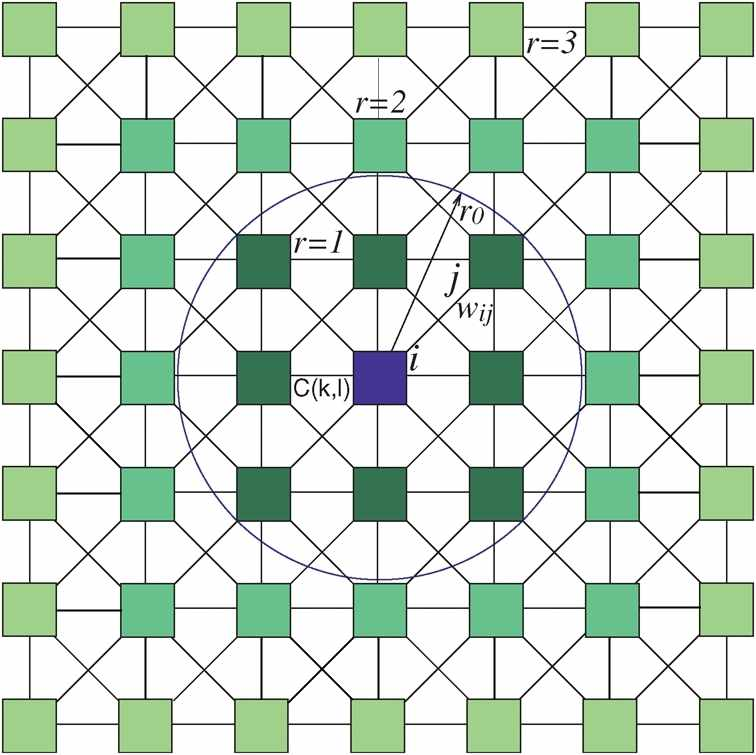
\includegraphics[width=0.5\textwidth]{fig/ccpp/nn_architecture2}
	\caption[Architecture of the 2D neural network.]{Architecture of the 2D neural network \citep{luo2008bioinspired}.}
	\label{fig:arch_nn}
\end{figure}

The dynamic activity of the $i$th neuron can be characterized by \citep{yang2004neural}
\begin{equation} \label{eq:binn}
\dot{x_i} = -A x_i + (B - x_i)\left([I_i]^{+} + \sum^k_{j=1}w_{ij}[x_j]^{+} \right) - (D+x_i)[I_i]^{-}
\end{equation}
where $A$, $B$, and $D$ are non-negative constants representing the passive decay rate and the upper and lower bounds of the neuron, i.e. $x_i \in [-D, B]$. $I_i$ is the external input to the $i$th neuron which can be defined as \citep{Scibilia2012}
\begin{equation}
I_i = 
\begin{cases}
\lambda_i E, & \text{if it is an unvisited area} \\
-E, & \text{if it is an obstacle area} \\
0, & \text{otherwise}
\end{cases}
\end{equation}
where $0 < \lambda_i \leq 1$ are scaling factors that can be used to prioritize certain areas, and $E$ is a constant such that $\lambda_i E \gg B$. The functions $[a]^{+}$ and $[a]^{-}$ are defined as $[a]^{+} = \max\{a,0\}$ and $[a]^{-} = \min\{-a,0\}$. $k$ is the number of neighboring neurons, and $x_j$ is a neuron in the neighborhood of $x_i$, i.e. $p_j \in \text{neig}_{r_0}(p_i)$. $w_{ij}$ is the connection weight between the $i$th and $j$th neuron defined as 
\begin{equation}
w_{ij} = \frac{\mu}{|p_i-p_j|}
\end{equation}
where $\mu > 0$ is a tuning constant. 

The neural connections $w_{ij}$ are defined in the design stage. Therefore, this neural network does not require any learning procedures. Neural connections only exist in the excitatory input $\left([I_i]^{+} + \sum^k_{j=1}w_{ij}[x_j]^{+} \right)$ in \eqref{eq:binn}. This means only positive neural activity can propagate. Consequently, uncovered areas globally attract, while obstacles only locally push away.

\subsection{Using the neural network for path planning}

Positive neural activity represents free uncovered areas. Deciding where to go next can then simply be done by going towards the most positive neuron at all times. Given the current position $p_q$ and heading $\theta_q$, \citet{Scibilia2012} suggest choosing the next position $p_n$ as
\begin{equation} \label{eq:binn_pos}
p_n \Leftarrow x_n = \argmax_{x_j:\ p_j \in \text{neig}_{r_0}(p_q)} \left\{ \left( 1 - \frac{\text{diff}(\theta_q,\theta_j)}{\pi} \right)\lambda x_j + (1-\lambda)x_j \right\}
\end{equation}
where $0 \leq \lambda \leq 1$ is a tuning constant which can be used to prioritize areas that do not require a change of direction. The function $\text{diff}(\theta_q,\theta_j)$ measures the smallest angle difference between $\theta_q$ and $\theta_j$. $\theta_j$ is the angle of the USV when it reaches $p_j$, and should be determined by the feasible path generation strategy employed. In this thesis, that means $\theta_j$ is the angle at the end of a simple Dubins path constructed from $p_q$ and $\theta_q$ to $p_n$. The computation of this angle is described in Section \ref{sec:pathgen}.

Complete coverage is then achieved by following the steps summarized in Algorithm 1. The steps are slightly modified from the algorithm presented in \citet{Scibilia2012} in order to incorporate the changes of \citet{luo2008bioinspired} and make it work for completely unknown environments.

\begin{tcolorbox}

\textbf{Algorithm 1: CCPP with bio-inspired neural network}

\emph{Input: Pose of USV, and rolling window map}

\begin{enumerate}
\itemsep0em

\item Partition the workspace into circular cells as described in Section \ref{sec:circle_partition}. Set the status of each cell to unknown, and mark all cells as uncovered.

\item Associate a neuron to each cell in the partition, and set all neural activities to zero.

\item Update the status of cells nearby the USV with information from the rolling window of Section \ref{sec:map_processing}.

\item If no reachable free cells remain, terminate the algorithm. Complete coverage has then been achieved. Else, continue with the substeps.
\begin{enumerate}
\itemsep0em

\item Update the status of cells nearby the USV with information from the rolling window of Section \ref{sec:map_processing}.

\item Evolve the neural network as in \eqref{eq:binn}.

\item Find next position as in \eqref{eq:binn_pos}. If the found next position is the same as the current position, stay still.

\item Mark the cell corresponding to the current position as covered.

\end{enumerate}

\item Go to step 4.

\end{enumerate}

\end{tcolorbox}


\section{Boustrophedon motions} \label{sec:ccpp_ba}

The proposed method solves the online complete coverage task in unknown workspaces using boustrophedon motions (i.e. a back-and-forth lawnmower pattern) and the A* search algorithm. The method works by first performing a boustrophedon motion in an uncovered region until a critical point is reached, i.e. a point where all nearby points are already covered or blocked by obstacles. To find a new uncovered region to cover, the method intelligently detects backtracking points based on accumulated knowledge. The best backtracking point is chosen as the starting point of the next boustrophedon motion, and an A* search is performed in order to reach the next starting point with the shortest collision-free path possible. When no backtracking points are detected, complete coverage is achieved. The usage of backtracking points is based on the work by \citet{Viet2013}, and minimizes the required number of boustrophedon motions before complete coverage is achieved. This method uses the square cell partitioning described in Section \ref{sec:square_partition}.

\subsection{Constructing the boustrophedon motion}

Collision-free motion is achieved by moving from one free cell to a neighboring free cell in the partition. When performing a boustrophedon motion, the algorithm's motion in the grid is defined by its moving direction (north or south) and its sweeping direction (east or west). The algorithm will start by moving straight forward in the moving direction until the next position is either blocked, or everything inside the coverage range is already covered. The boustrophedon motion is illustrated in \figref{fig:bm_dir}.

When the algorithm can no longer move straight forward it will try to perform wall following. If there are uncovered free cells in the sweeping direction, the algorithm will perform wall following in the sweeping direction. If no uncovered free cells are found, the sweeping direction is switched: from east to west or from west to east. Wall following is then attempted again in the new sweeping direction. If the algorithm still cannot find uncovered free cells, a critical point has been reached and the algorithm backtracks if possible.

If the algorithm decides to wall follow, it will move in the sweeping direction twice the number of cells covered by the shortest coverage range on the current lap.
For example, if the algorithm detects a wall after moving north with a coverage range that varies between 3 and 4 cells, the algorithm will wall follow 6 cells in the sweeping direction. This approach to variable inter-lap spacing is inspired by \citet{galceran2012efficient}, and minimizes the overlapping sensor coverage. When the desired number of cells is reached, or the algorithm is blocked from moving further, wall following is finished. The moving direction is then switched: from north to south or from south to north, and the algorithm starts on a new lap. The boustrophedon motion is summarized in Algorithm 2.

\begin{figure}[h!]
	\centering
	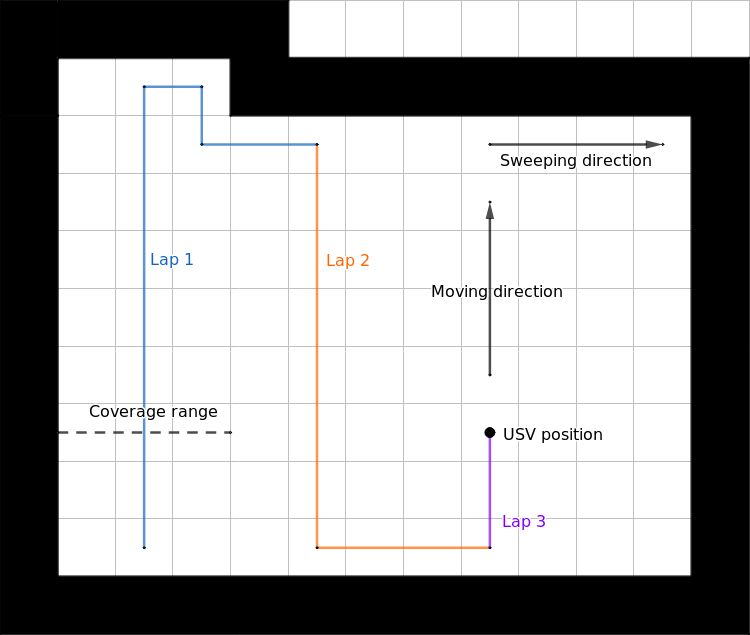
\includegraphics[width=0.5\textwidth]{fig/ccpp/bm_desc}
	\caption[Boustrophedon motion with a symmetric constant coverage range.]{Boustrophedon motion with a symmetric constant coverage range. White cells are free and black cells are obstacles.}
	\label{fig:bm_dir}
\end{figure}

\begin{tcolorbox}

\textbf{Algorithm 2: Constructing a boustrophedon motion}

\emph{Input: Pose of USV, coverage range, partitioned workspace, and rolling window map}

\begin{enumerate}
\itemsep0em

\item Check one step along the moving direction.
\begin{enumerate}
\itemsep0em

\item If the cell is free and the current coverage range ensures that new cells are covered by moving to it: move one cell along this direction. Then go to step 2. Else, continue.

\item If the cell is blocked and uncovered free cells are available in the sweeping direction: wall follow one cell in the sweeping direction. Then go to step 2. Else, continue.

\item If the cell is blocked and uncovered free cells are available opposite of the sweeping direction: switch sweeping direction and wall follow one cell in the new sweeping direction. Then go to step 2. Else, continue.

\item A critical point has been reached. Terminate the algorithm.

\end{enumerate}
\itemsep0em

\item Mark cells as covered based on the coverage range and method of Section \ref{sec:handle-mbes}.

\item Update the status of cells nearby the USV with information from the rolling window of Section \ref{sec:map_processing}. Go to step 1.

\end{enumerate}

\end{tcolorbox}



\subsection{Determining the backtracking point}

Complete coverage most often requires multiple boustrophedon motions. After finishing a motion, a backtracking point needs to be determined as the starting point of the next boustrophedon motion. This can generally be at any free uncovered cell in the grid map. However, choosing the next starting point wisely can reduce the amount of boustrophedon motions required to achieve complete coverage. \citet{Viet2013} therefore suggest a strategy of choosing candidate backtracking points where the surrounding 8 cells are considered. Let $s_i$ with $i=1,2,...8$ be the surrounding cells as in \figref{fig:bps}. A backtracking point is then detected if $\mu (s) \geq 1$ where
\begin{multline} \label{eq:bp1}
\mu (s) = b(s_1,s_8)+b(s_1,s_2)+b(s_3,s_2)+b(s_3,s_4)+b(s_5,s_6) \\ 
+b(s_5,s_4)+b(s_7,s_6)+b(s_7,s_8)
\end{multline}
and
\begin{equation} \label{eq:bp2}
b(s_i,s_j) = 
\begin{cases}
1, & \text{if ($s_i$ is free) and ($s_j$ is blocked)} \\
0, & \text{otherwise.}
\end{cases}
\end{equation}
Note that \eqref{eq:bp1} is modified to also include $s_3$, since the proposed method does not use the same north-south-east-west priority as \citet{Viet2013}. Among these candidates, the backtracking point is chosen as the candidate with the shortest distance to the current critical point. In this thesis, the backtracking point with the shortest path using an A* search is chosen. If no backtracking points are found, complete coverage is achieved and the method is finished. 

\begin{figure}[h!]
	\centering
	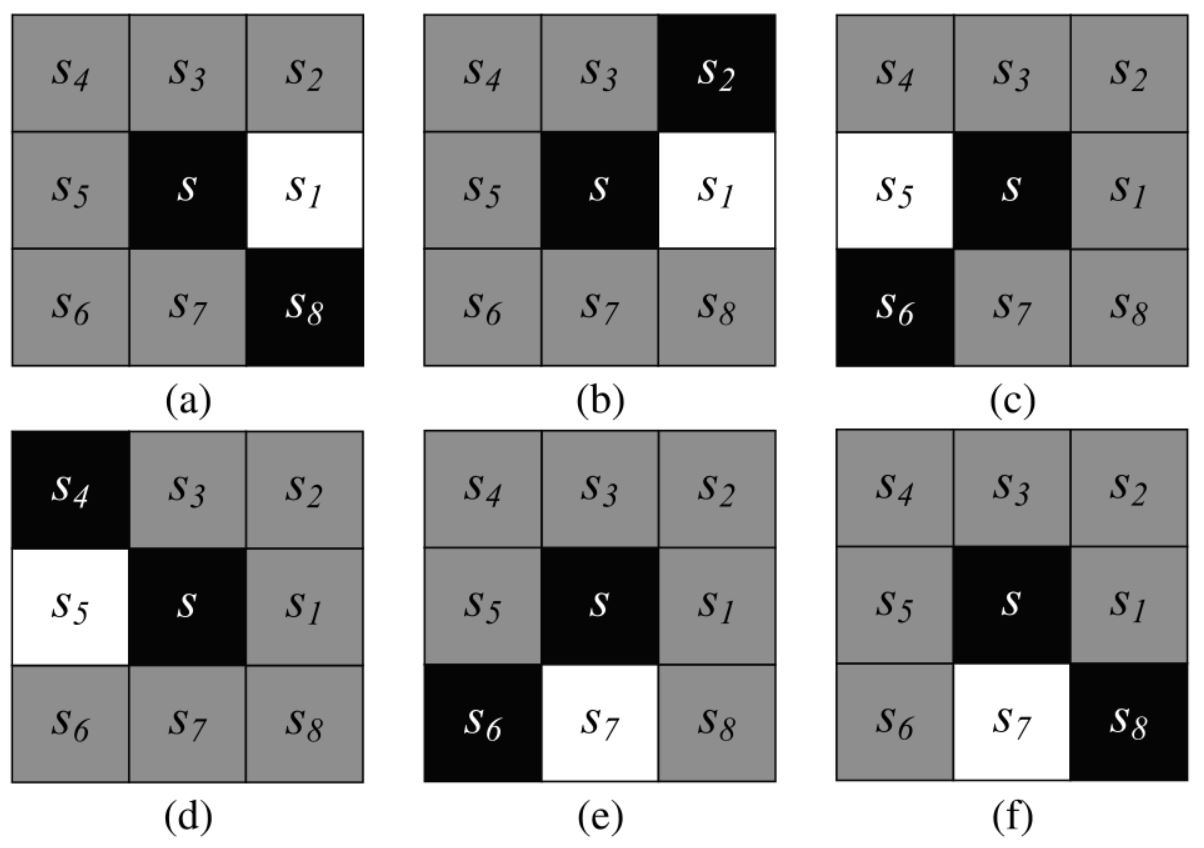
\includegraphics[width=0.5\textwidth]{fig/ccpp/bps}
	\caption[Conditions for backtracking points.]{Conditions for backtracking points \citep{Viet2013}. White tiles are free, black tiles are either covered or obstacle, gray tiles can be anything.}
	\label{fig:bps}
\end{figure}

The approach of \citet{Viet2013} assumes that one cell represents the coverage of a vacuum cleaner. However, the proposed method of this thesis assumes a varying coverage range sensor, and the proposed square cell partitioning allows multiple cells to be marked as covered. Thus, the backtracking point should be adjusted so that the distance between the new lap and the closest lap is twice the shortest coverage range of the latter.

\subsection{Planning a path to the backtracking point}

Planning a path from the critical point to the backtracking point can be done with a shortest path searching algorithm. The A* algorithm is a popular choice in robotic applications, and a description of the algorithm can easily be found online \citep{wiki:a_star}. By performing the search exclusively over free and already covered cells, the resulting path is guaranteed free of static obstacles. If it is discovered that a moving obstacle has obstructed the backtracking path, a new backtracking point is determined and the path is replanned from the current position. 

A* traverses the partitioned grid map one cell at a time. The low resolution of the cells will therefore lead to a path that is longer and has more turns than necessary. Inspired by \citet{Viet2013}, a smoothing of the path is done by removing the cells between any two cells with line-of-sight. Determining line-of-sight between two cells can be done by using the supercover line algorithm introduced for the square cell partitioning in Section \ref{sec:square_partition}. Line-of-sight is then achieved if none of the tiles intersected by the supercover line is an obstacle. The algorithm for smoothing the A* path is described in \citet{Viet2013}. \figref{fig:backtracking} shows the difference between a smoothed and non-smooth backtracking path. The resulting online CCPP algorithm is summarized in Algorithm 3.

%\todo[inline]{TODO: The backtracking point at the top of the map is the closest. Change figure.}

\begin{figure}[h!]
    \centering
	\makebox[\linewidth][c]{
	\begin{subfigure}[b]{0.5\textwidth}
		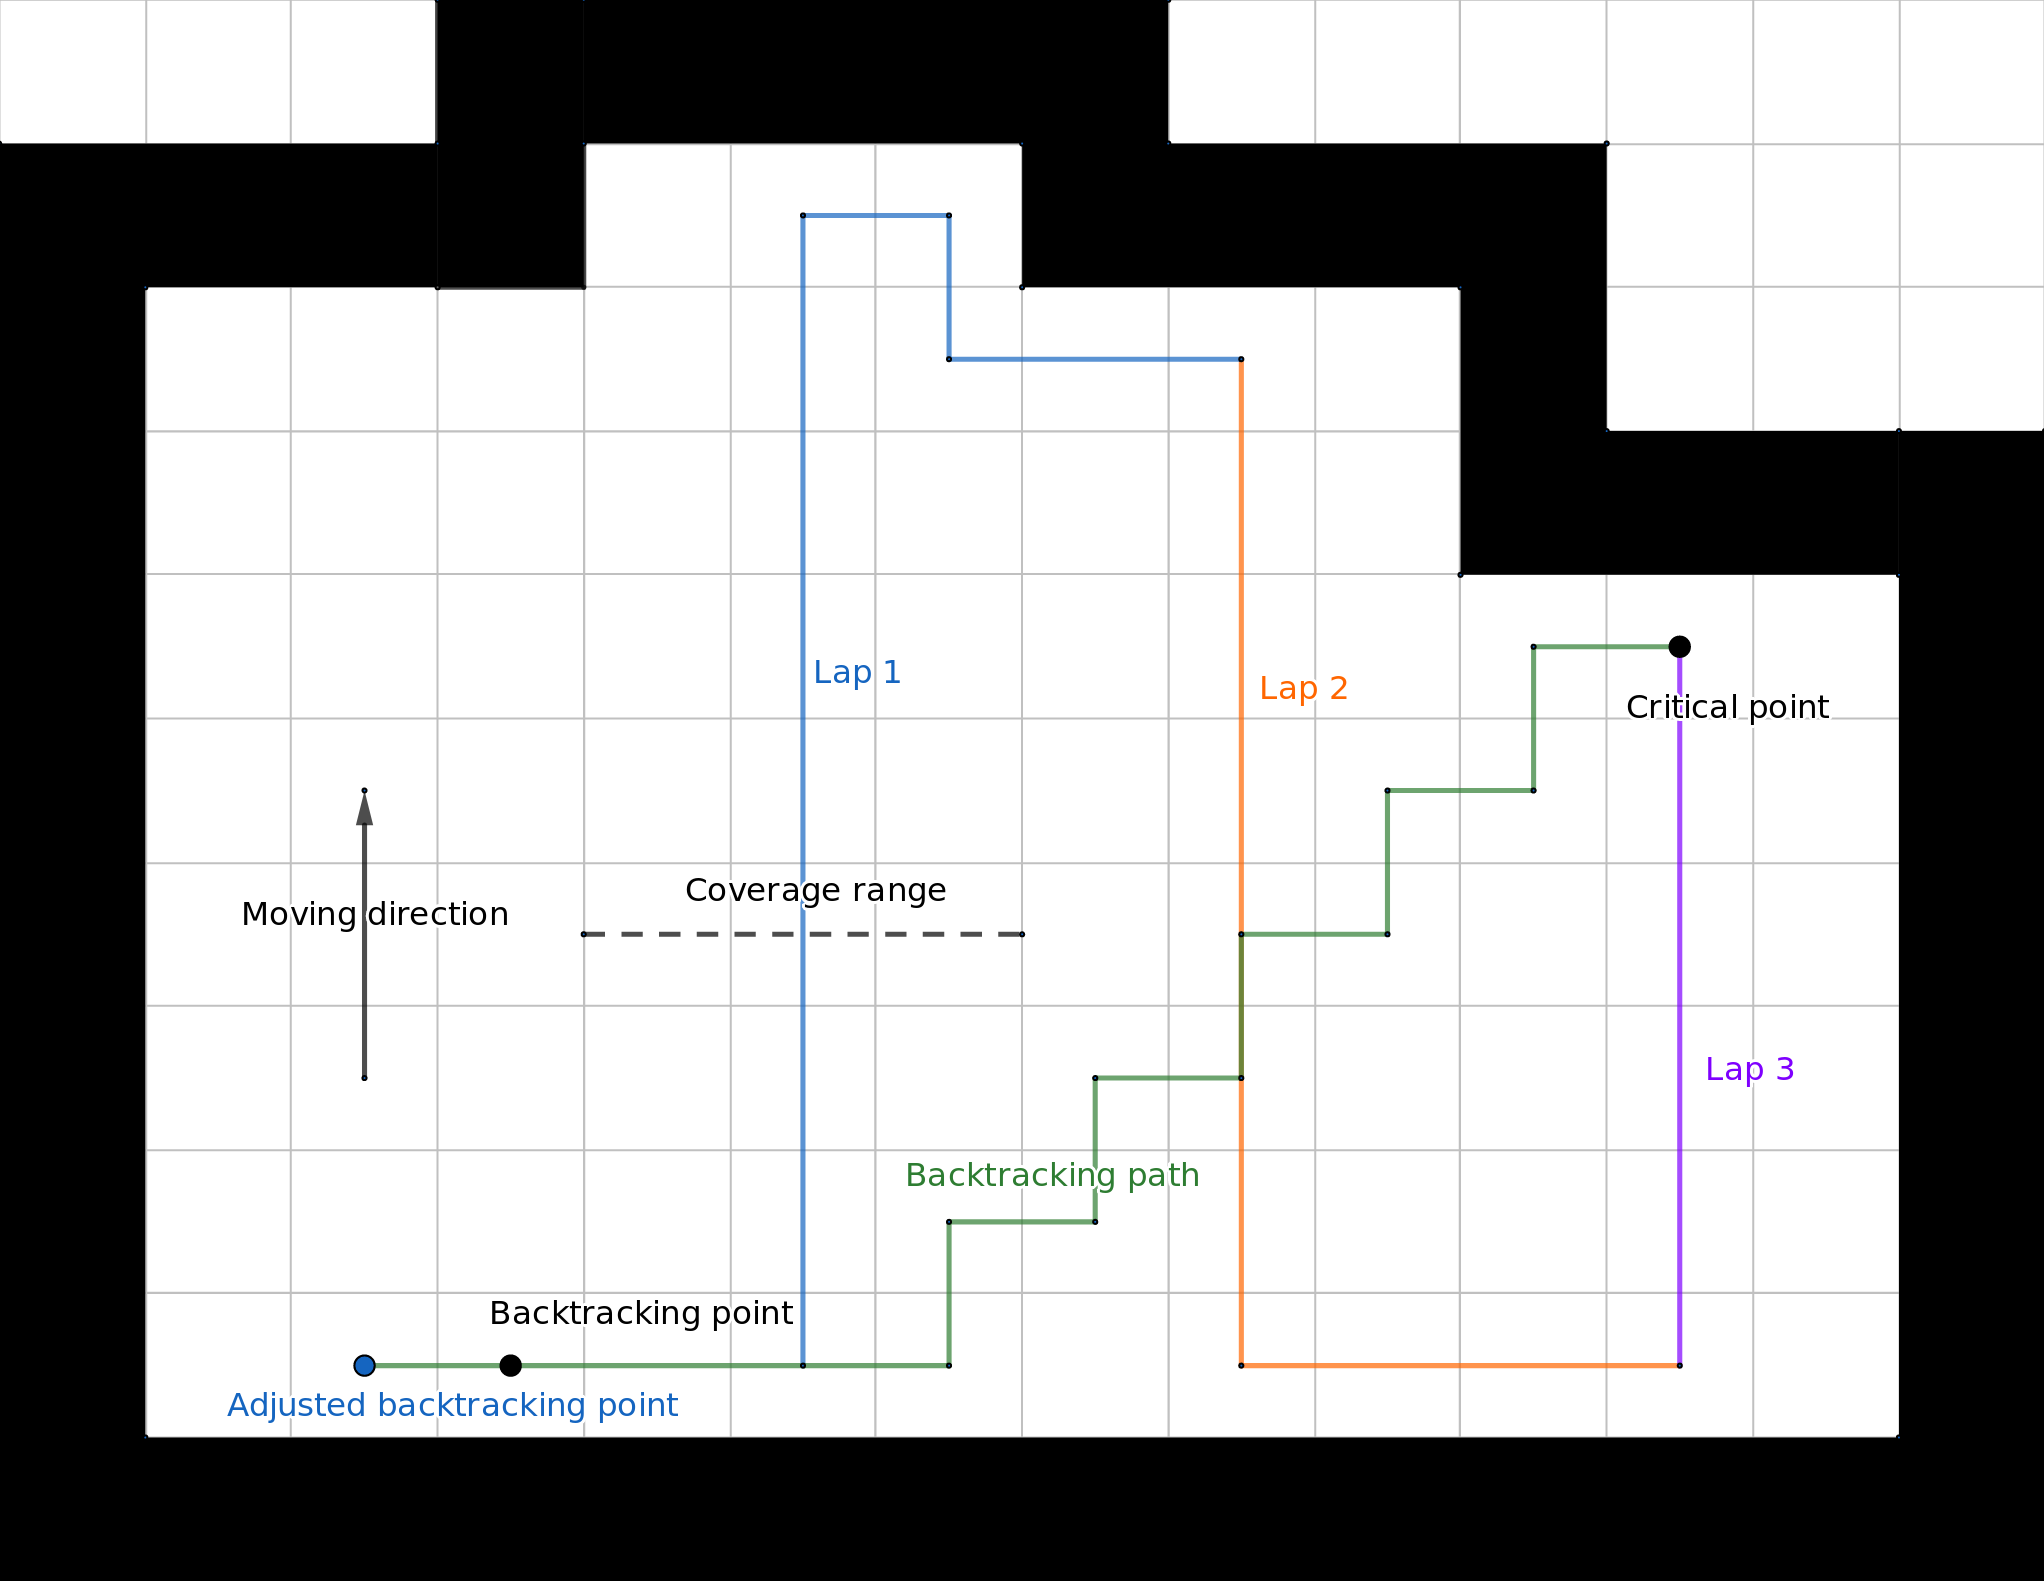
\includegraphics[width=1\linewidth]{fig/ccpp/backtracking_2}
		\caption{}
	\end{subfigure}
	\begin{subfigure}[b]{0.5\textwidth}
		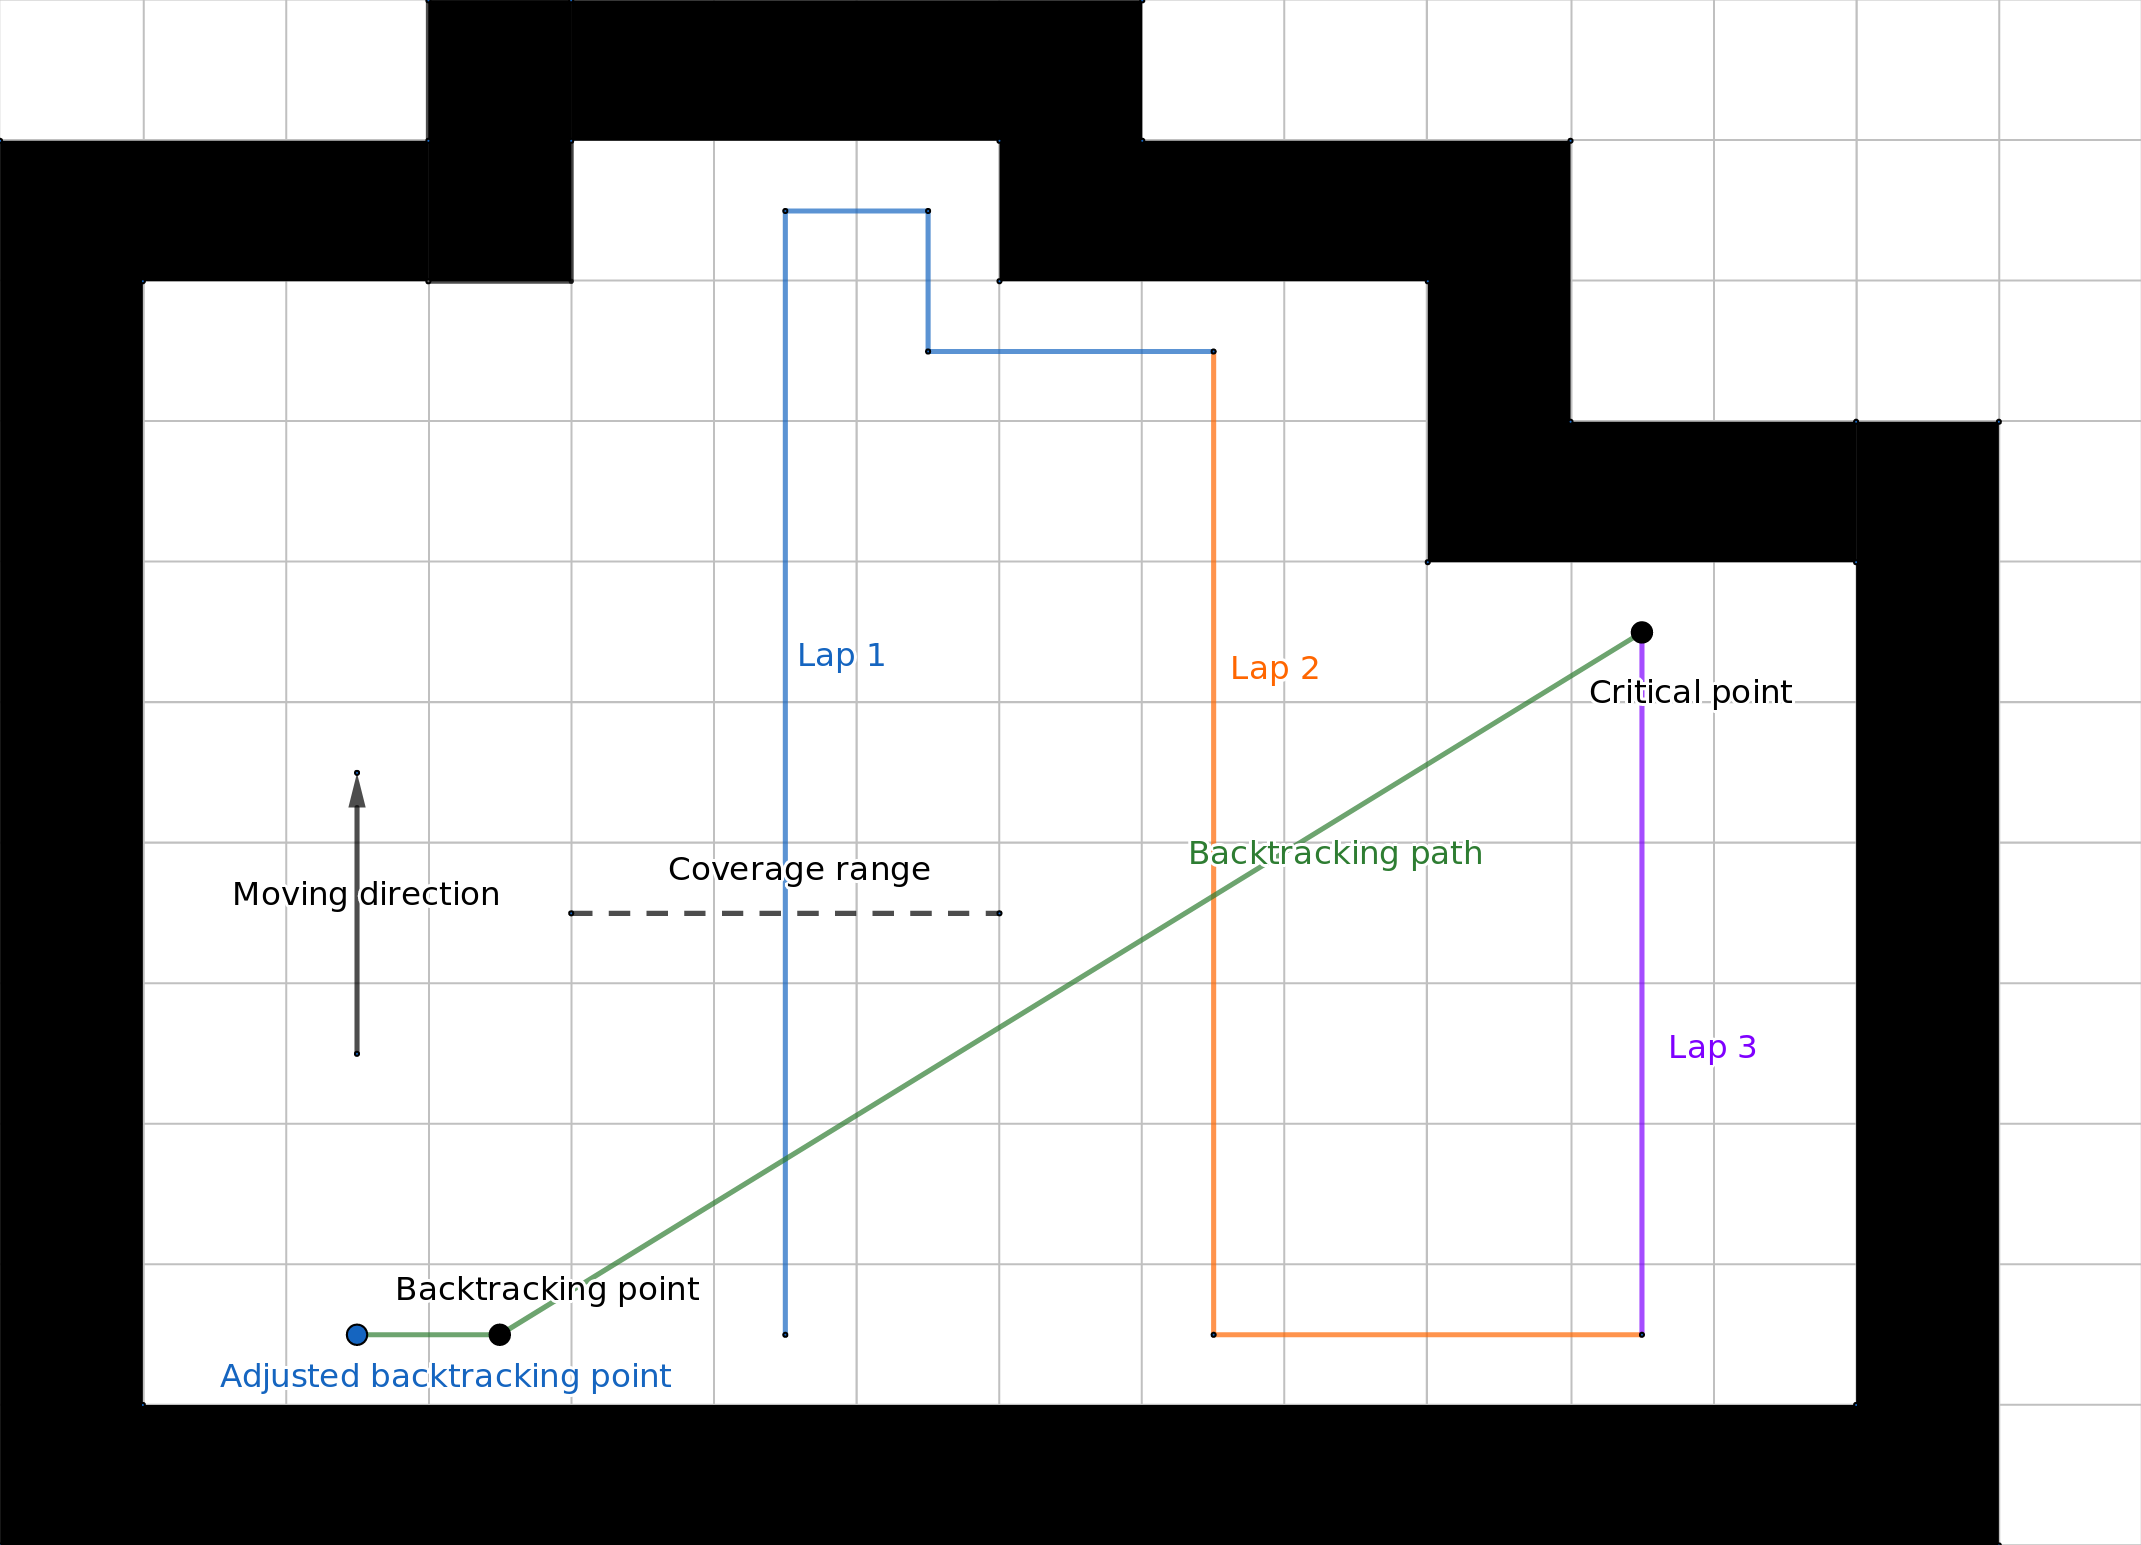
\includegraphics[width=1\linewidth]{fig/ccpp/backtracking_1}
		\caption{}
	\end{subfigure}
	}
	\caption[Smoothing of the A* backtracking path.]{A* smoothing. White cells are free and black cells are obstacles. (a) A non-smooth A* backtracking path. (b) The backtracking path is smoothed by removing cells between other cells with line-of-sight.} \label{fig:backtracking}
\end{figure}

\begin{tcolorbox}

\textbf{Algorithm 3: CCPP with boustrophedon motions}

\emph{Input: Pose of USV, and rolling window map }

\begin{enumerate}
\itemsep0em

\item Partition the workspace into square cells as described in Section \ref{sec:square_partition}. Set the status of each cell to unknown, and mark all cells as uncovered.

\item Begin to cover the workspace with a boustrophedon motion as described in Algorithm 2. The boustrophedon motion is finished when the algorithm arrives at a critical point.

\item With the accumulated knowledge from step 2, detect backtracking points according to \eqref{eq:bp1} and \eqref{eq:bp2}. If no backtracking points are found, complete coverage is achieved. Terminate the algorithm. Else, continue with the next step.

\item Determine the best backtracking point by finding the point requiring the shortest A* path. Apply line-of-sight smoothing to the shortest path.

\item Follow the smoothed A* path to the next starting point. Replan if it becomes blocked. Go to step 1.

\end{enumerate}

\end{tcolorbox}



\chapter{Guidance and path generation}

The CCPP methods described in the previous chapter generate only one waypoint ahead in time. The next waypoint is determined only after the USV has reached its current waypoint. This motivates an online feasible path generation strategy. Upon each new waypoint, a feasible path is generated from the current USV pose to the next waypoint. A distinction is made here between path planning, as the generation of waypoints, and path generation, as the generation of a smooth curve between two points. To ensure that this curve is feasible, the USV's turning radius and speed must be taken into account. Given the curve from the path generation strategy, a guidance law generates continuous course and speed control that is passed on to the USV's onboard system.  

\section{Feasible path generation using straight lines and arc segments} \label{sec:pathgen}

A simple Dubins path consists of an arc segment followed by a straight line. This path is the shortest path that can be generated from a configuration (position and heading) to a position \citep{Scibilia2012}. Given the initial position and heading $p_q = (x_q, y_q)$ and $\theta_q$ and the final position $p_n$, the aim is to find the shortest path from $p_q$ to $p_n$ with initial heading $\theta_q$. Furthermore, the turning radius $\rho$ of the arc segment must be greater than the minimum feasible turning radius of the USV, i.e. $\rho \geq \rho_{min}$, where $\rho_{min}$ is the turning radius at the minimum required operating speed of the USV. The turning radius $\rho$ is a design parameter.

%If the minimum feasible turning radius of the USV, $\rho_{min}$, is smaller than half the distance between the start and end point, i.e. $\rho_{min} < \frac{|p_q - p_n|}{2}$, a simple Dubins path can be constructed. This places a constraint on the distance between subsequent waypoints generated by the CCPP method

\subsection{Turning direction}

Consider the straight line defined by the initial position and heading. The distance from $p_n$ to this line is given by 
\begin{equation}
	e_{nq} = -[x_n - x_q]\sin(\theta_q) + [y_n - y_q]\cos(\theta_q).
\end{equation}
The turning direction $\delta$ can be determined checking the sign of $e_{nq}$, 
\begin{equation}
\delta = 
\begin{cases}
1, & \text{if } e_{nq} > 0 \\
-1, & \text{otherwise.}
\end{cases}
\end{equation}
The value $\delta = 1$ corresponds to a left turn, and $\delta = -1$ corresponds to a right turn (z-axis assumed positive upward).

\subsection{Center of turning circle}

The arc segment is a segment of a turning circle which is located on a line perpendicular to the heading line and that goes through $p_q$. The coordinates for the center of the turning circle are given by
\begin{equation}
p_c = (x_c, y_c) = 
\begin{cases}
(x_q + \sin(\theta_q)\rho, y_q - \cos(\theta_q)\rho), & \text{if it is a right turn}  \\
(x_q - \sin(\theta_q)\rho, y_q + \cos(\theta_q)\rho), & \text{if it is a left turn,} 
\end{cases}
\end{equation}
and the circle has a radius $\rho$. In order for a Simple Dubins path to be constructed, the turning radius $\rho$ must be small enough such that the final position $p_n$ is not located inside the turning circle. Ensuring that the turning radius $\rho$ is smaller than half the distance between the start and end point, i.e. $\rho_{min} < \frac{|p_q - p_n|}{2}$, is a sufficient condition that can be imposed by properly choosing the distance between waypoints in the CCPP methods.

\subsection{Tangent point}

The arc segment starts in $p_q$ and follows the turning circle in the turning direction. The end point of the arc segment, however, is still unknown. This is determined by one of the tangent points generated by the tangent lines from the final position $p_n$ to the circle. The two lines tangent to the turning circle can be found by geometrical considerations, for instance by solving the second order trigonometric equation \citep{Scibilia2012}
\begin{equation}
((x_c - x_n)\sin(\beta) + (y_n - y_c)\cos{\beta})^2 = \rho^2,
\end{equation}
where $\beta$ is the angle of the tangent line. From this, two tangent points are obtained, and the first one encountered along the direction of rotation is used as the endpoint of the arc segment, denoted $p_l$. The geometry of the Simple Dubins path is shown in \figref{fig:dubins_ex}.

\begin{figure}[h!]
	\centering
	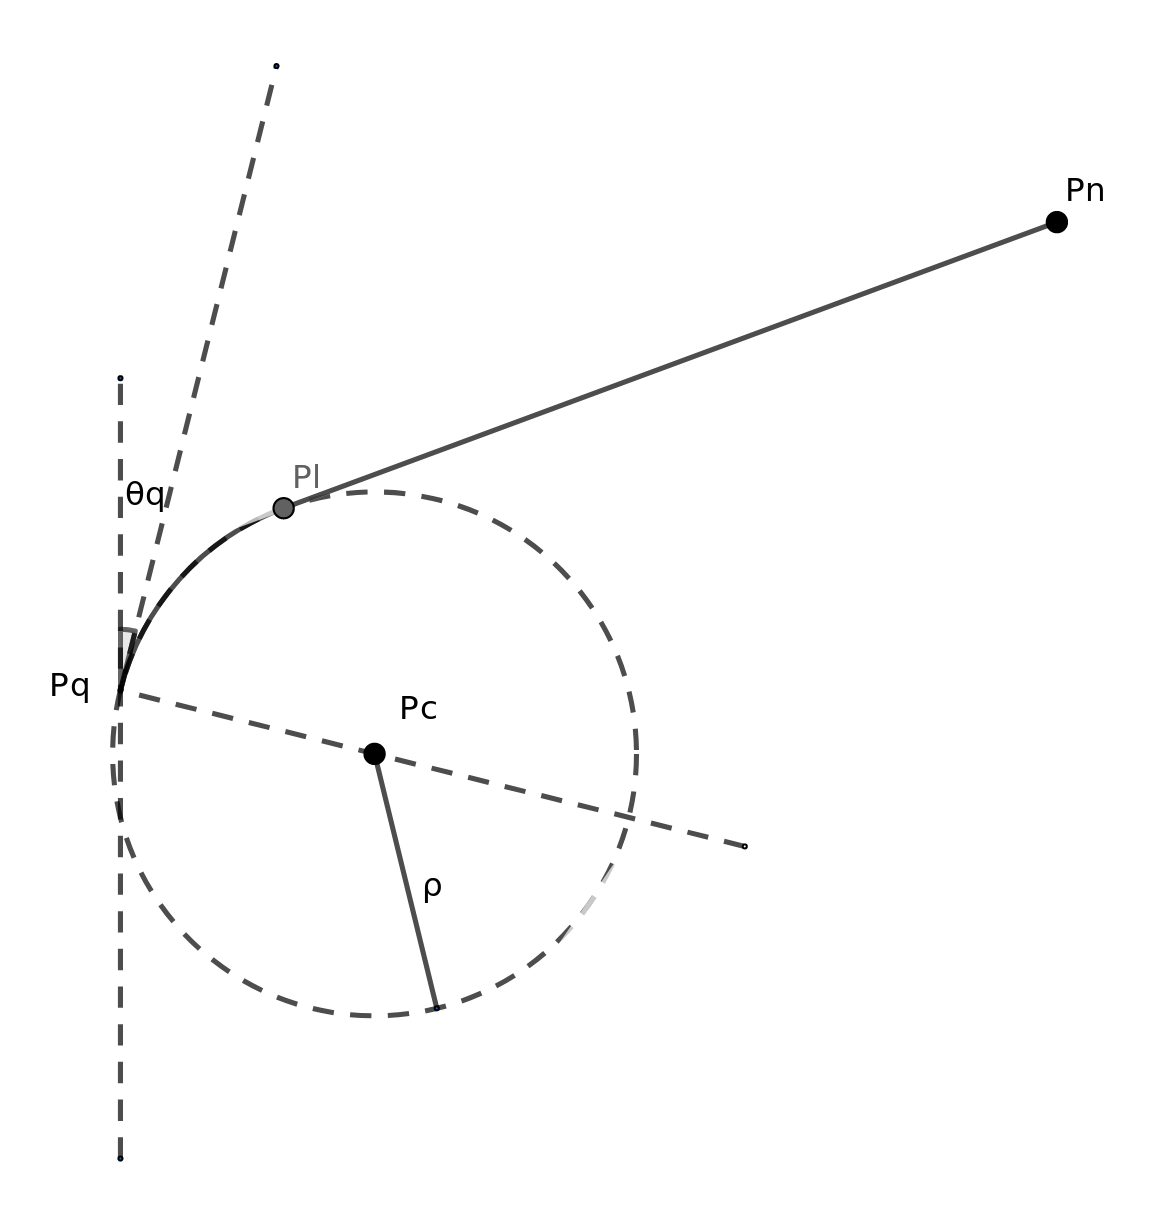
\includegraphics[width=0.5\textwidth]{fig/guidance/dubins}
	\caption{Simple Dubins path geometry.}
	\label{fig:dubins_ex}
\end{figure}

\subsection{Generating the path}

In ROS, a path is described by a \path{nav_msgs/Path} message, which consists of an array of poses. Now that the turning direction, turning circle and tangent point are known, generating poses on the path is trivial. The final heading of the path becomes
\begin{align}
	\theta_n = \text{atan2}(y_n - y_l, x_n - x_l)
\end{align}
where atan2 is a generalization of arctan that also determines the correct quadrant. The resolution of the generated path in the implemented system, i.e. the distance between consecutive poses, is determined by a user-specified parameter. A simple Dubins path can be seen in \figref{fig:dubins_rviz}.

\begin{figure}[h!]
	\centering
	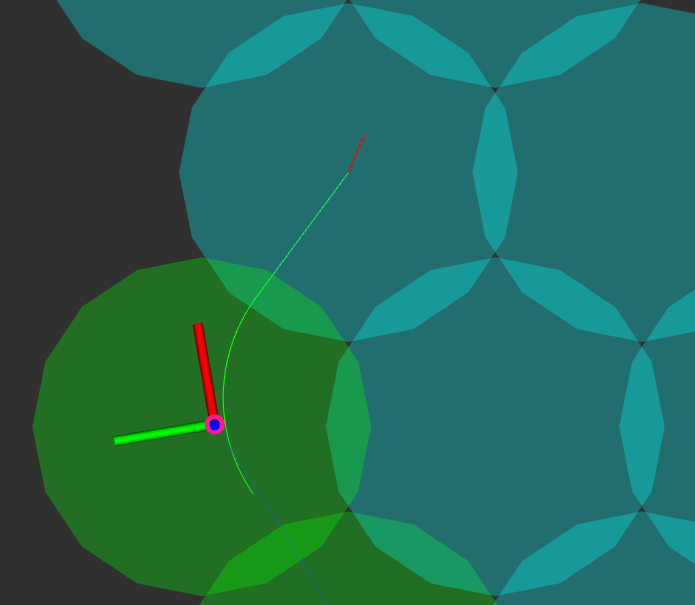
\includegraphics[width=0.5\textwidth]{fig/guidance/dubins-path}
	\caption{A generated simple Dubins path (green curve).}
	\label{fig:dubins_rviz}
\end{figure}



\section{Curved path line-of-sight guidance law with time-varying lookahead distance}

The guidance law will keep the USV on the path, or lead it towards the path if the position error is nonzero. The input to the guidance law is the path generated in Section \ref{sec:pathgen}, and the outputs are speed and course assignments. \figref{fig:los-geometry} shows the geometry of the curved path LOS guidance problem and some of the variables involved. The method presented in this section is based on \citet{lekkas2014integral}. 

\begin{figure}[h!]
	\centering
	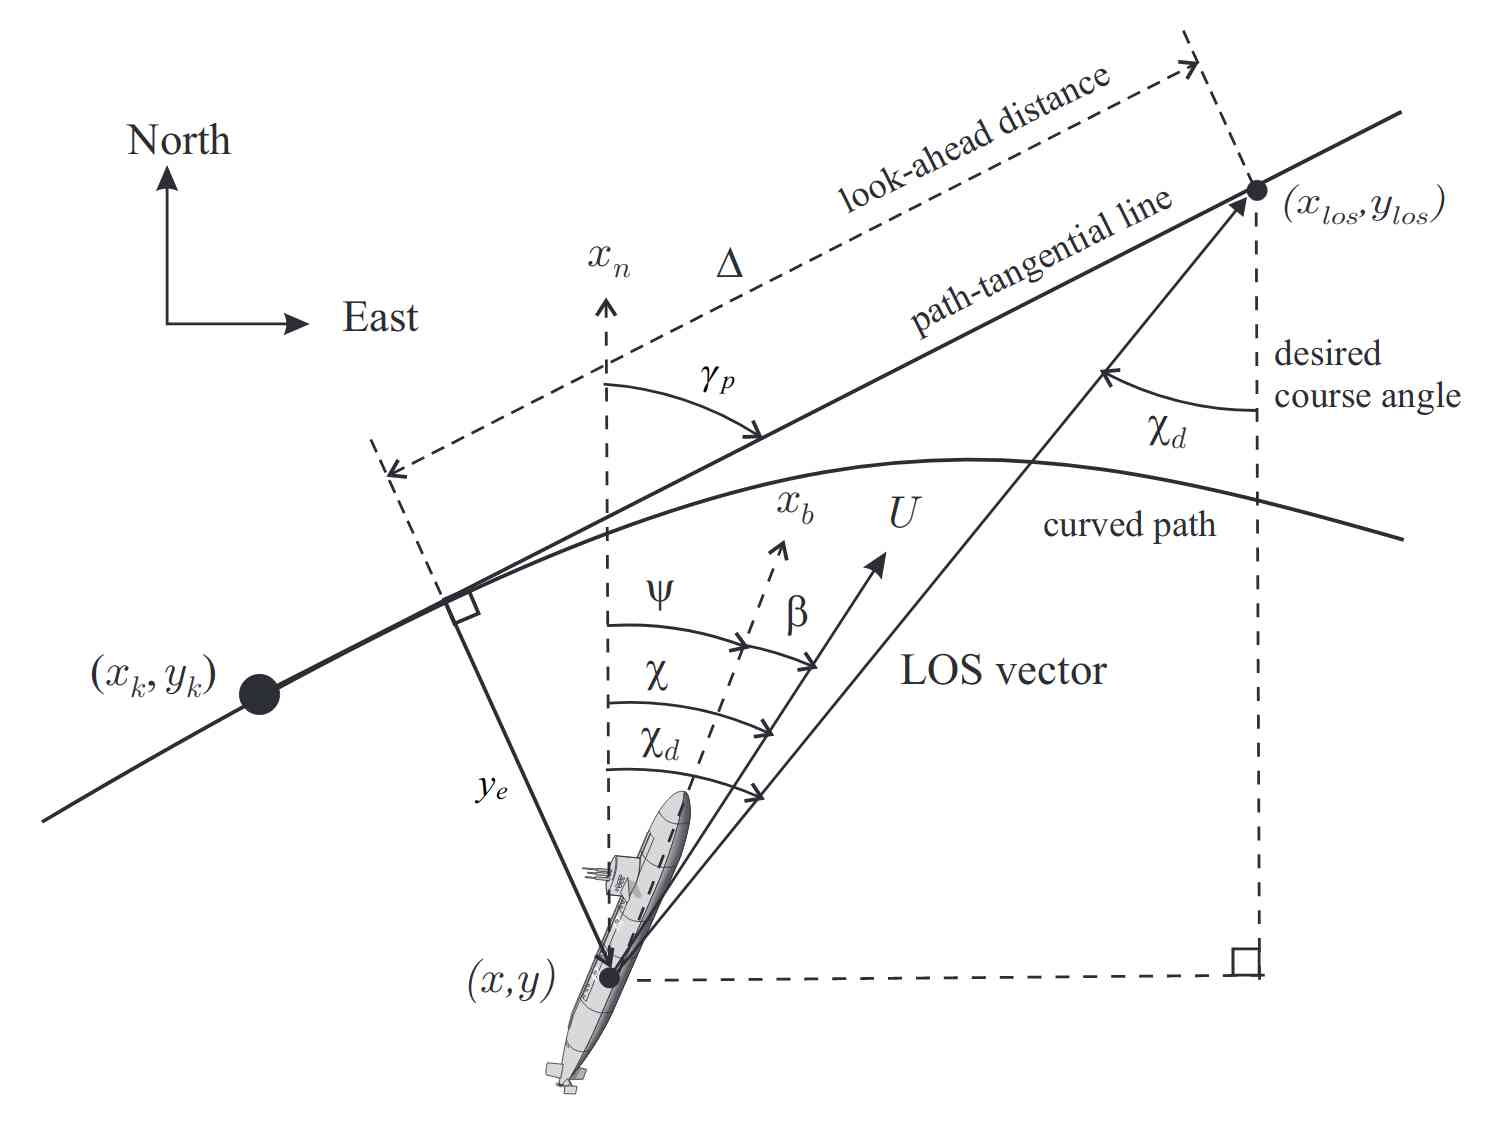
\includegraphics[width=0.7\textwidth]{fig/guidance/curved-guidance.jpg}
	\caption[Line-of-sight guidance geometry for curved paths.]{Line-of-sight guidance geometry for curved paths \citep{lekkas2014integral}.}
	\label{fig:los-geometry}
\end{figure}

\subsection{Cross-track error}

The cross-track error is the orthogonal distance from the USV position $(x,y)$ to a path-tangential reference frame defined by a point $(x_p,y_p)$ and rotated an angle $\gamma_p$ about the z-axis. The point $(x_p, y_p)$ is the point on the path that is closest to the USV position
\begin{equation}
(x_p,y_p,\theta_p) = \argmin_{(x_i,y_i,\theta_i) \ \in \ P} \sqrt{(x_i - x)^2 + (y_i - y)^2}
\end{equation} 
where $P = [(x_1,y_1,\theta_1), (x_2,y_2,\theta_2), ... , (x_n,y_n,\theta_n)]$ is the path, and $n$ is the number of poses in the path. The path tangential angle at any point on the path is then given by $\gamma_p = \theta_p$. The cross-track error can be computed by
\begin{equation}
y_e = -(x - x_p)\sin(\gamma_p) + (y - y_p)\cos(\gamma_p).
\end{equation}
The control objective for curved path following then becomes
\begin{equation}
\lim_{t \to +\infty} y_e(t) = 0.
\end{equation}

\subsection{Guidance law}

An LOS vector is constructed from the USV to a point $(x_{los}, y_{los})$ located on the path-tangential line. The distance from the closest point on the path $(x_p,y_p)$ to $(x_{los},y_{los})$ depends on a lookahead distance $\Delta(t) > 0$. From geometric consideration of \figref{fig:los-geometry}, the guidance law is given by
\begin{equation} \label{eq:guidance_law}
\chi_d = \gamma_p + \text{arctan}\left( \frac{-y_e}{\Delta} \right)
\end{equation}
where $\chi_d$ is the desired course angle of the USV defined as
\begin{equation}
\chi_d = \psi_d + \beta.
\end{equation} 
$\psi_d$ is the desired heading angle and $\beta$ is the sideslip angle. Sideslip is the deviation between where the USV is looking (heading), and the direction it is moving (course). It is caused by a nonzero sway velocity component, and occurs due to external forces such as currents, or lateral accelerations while turning. Since the Otter USV's onboard system uses course control, this is already compensated for.

\subsection{Time-varying lookahead distance} 

From \figref{fig:los-geometry} it is easy to see that a small lookahead distance results in a more aggressive steering, i.e. the desired path is reached faster. However, it will also contribute to unwanted oscillations around the path. A large lookahead distance produces smoother steering which avoids oscillations, but it also means that it takes longer to converge to the path. This motivates the use of a time-varying lookahead distance. By implementing a time-varying lookahead distance, the goal is to keep both the advantage of a faster convergence rate, and the reduction in unwanted oscillations. \citet{lekkas2014integral} proposes the following formula
\begin{equation} \label{eq:delta}
\Delta(y_e) = (\Delta_{max} - \Delta_{min}) e^{-K_\Delta y_e^2} + \Delta_{min}
\end{equation} 
where $\Delta_{max}$ and $\Delta_{min}$ are the maximum and minimum values for $\Delta$. The convergence rate $K_\Delta$, along with $\Delta_{max}$ and $\Delta_{min}$ constitute design parameters to be set by the user. 

\eqref{eq:delta} works by assigning a small value to $\Delta$ when the USV is far from the desired path, and a large value when it is close to the path. Since a small $\Delta$ results in aggressive steering, the USV will quickly converge towards the path when it is far away. Similarly, when the USV close to the path, a large $\Delta$ results in smoother steering which gives smaller overshoot and fewer oscillations. As opposed to a constant lookahead distance $\Delta$, \eqref{eq:delta} increases the number of design parameters that must be determined by the user.

\subsection{Speed assignment}

The following speed assignment is proposed
\begin{equation}
U_d = \max(U_{max} * (1 - \frac{|y_e|}{y_{max}} - \frac{|\tilde{\chi}|}{\chi_{max}}) + U_{min}, U_{min})
\end{equation}
where $U_d$ is the desired speed, $U_{max}$ and $U_{min}$ are the upper and lower limits for the speed, $y_e$ is the cross-track error, and $\tilde{\chi} = \chi - \chi_d$ is the error in the course angle. $y_{max}$ and $\chi_{max}$ are design parameters for the maximum allowed cross-track error and course angle error before the speed is assigned its minimum possible value.

This speed assignment ensures that the speed is lowered when the USV deviates from its path. With a lower speed the turning radius decreases, which in turn makes it easier for the USV to get back on the desired path. When the speed reaches its minimum, i.e. $U = U_{min}$, the USV will achieve its minimum turning radius $\rho_{min}$ which ensures that any generated path can be followed. An additional benefit is that when the USV tracks the path well, the speed is increased in order to save time.

\subsection{Interfacing with the Otter USV's thrusters}

The guidance system must be connected to the Otter USV's onboard system, since the onboard system already contains the thrust allocation strategies and low-level controllers required to steer the USV. The onboard system has therefore been modified to accept speed and course assignments over UDP. Similarly, the guidance system is extended to send these messages. The messages are serialized based on Google's Protocol Buffers \citep{wiki:protobuf}, which is a simple and effective way of communicating between different systems.

Before the messages can be sent, however, the desired course angle in the SLAM map's coordinate frame must be converted to an angle in the NED frame. The difference between the coordinate frames is just an offset, and can be adjusted for as follows
\begin{equation}
\chi_d = \chi_d^{SLAM} - \chi^{SLAM} + \chi 
\end{equation}
where $\chi$ and $\chi_d$ are the course and desired course angle in NED, and $\chi^{SLAM}$ and $\chi_d^{SLAM}$ are the course and desired course angle in the SLAM map's coordinate frame.

\chapter{Simulations}

\section{Simulator}

A simulation environment for the USV has been set up in ROS Melodic and Gazebo 9. The simulator supports altering of the system matrices and thruster configuration. Simulated input can be provided from several sensors, including GNSS, IMU, and 2D lidar. The surrounding environment can be modified by adding and removing obstacles. The simulator is based on the Virtual RobotX simulator \citep{website:vrx}, and the theory of its operation is available in \citet{website:vrx_to}.

\section{Map generation with SLAM}

\figref{fig:sim_sensor_fusion}b shows the map generated by Cartographer after moving the USV along the edges of the area in \figref{fig:sim_sensor_fusion}a. The middle of the map is unknown due to the lidar's inability to detect across the middle.

\begin{figure}[h!]
    \centering
	\makebox[\linewidth][c]{
	\begin{subfigure}[b]{0.5\textwidth}
		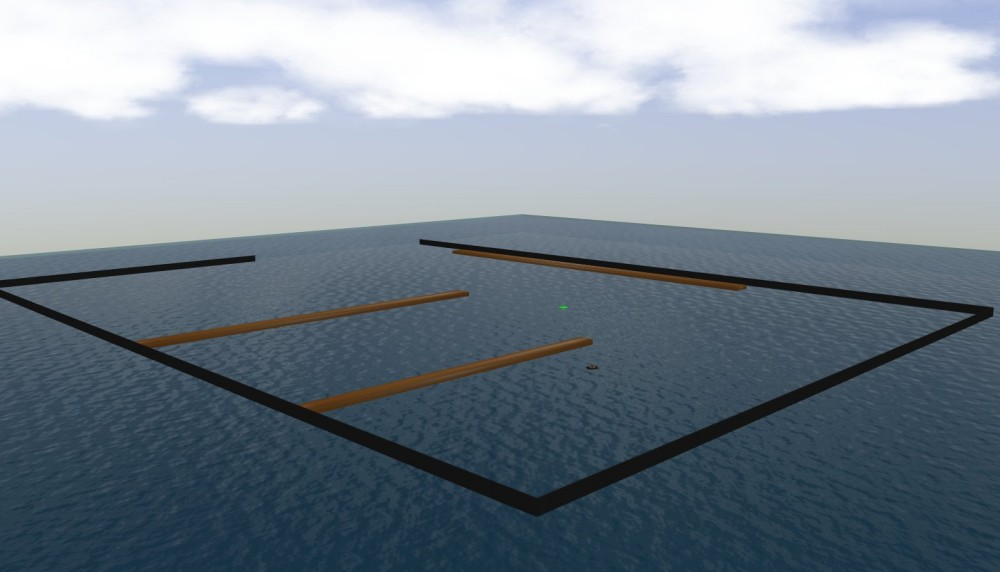
\includegraphics[width=1.0\textwidth,height=0.185\textheight]{fig/simulations/env2}
		\caption{}
	\end{subfigure}
	\begin{subfigure}[b]{0.5\textwidth}
		
\includegraphics[width=1.0\textwidth]{fig/simulations/env_slam2}
		\caption{}
	\end{subfigure}
	}
	\caption[Map generation with SLAM of a simulated environment.]{(a) Simulation environment. (b) SLAM map. The white area of the map represents free space, the black area represents obstacles, and the dark gray area in the middle is unknown. The black area is hard to see, but is located at the most distinct transitions from white to dark gray.}
	\label{fig:sim_sensor_fusion}
\end{figure} 

\section{Complete coverage maneuvering with boustrophedon motions}

\subsection{Constant coverage range} \label{sec:sim1}

The target region and surrounding environment for this simulation is shown in \figref{fig:target_region_bm_1}. A symmetric constant coverage range of $\SI{10}{\meter}$  is assumed for the MBES, i.e. $\SI{5}{\meter}$ in both starboard and port directions. The simulated lidar has a range of $\SI{25}{\meter}$, which is the same as the lidar in the real-world experiments.

\begin{figure}[h!]
	\centering
	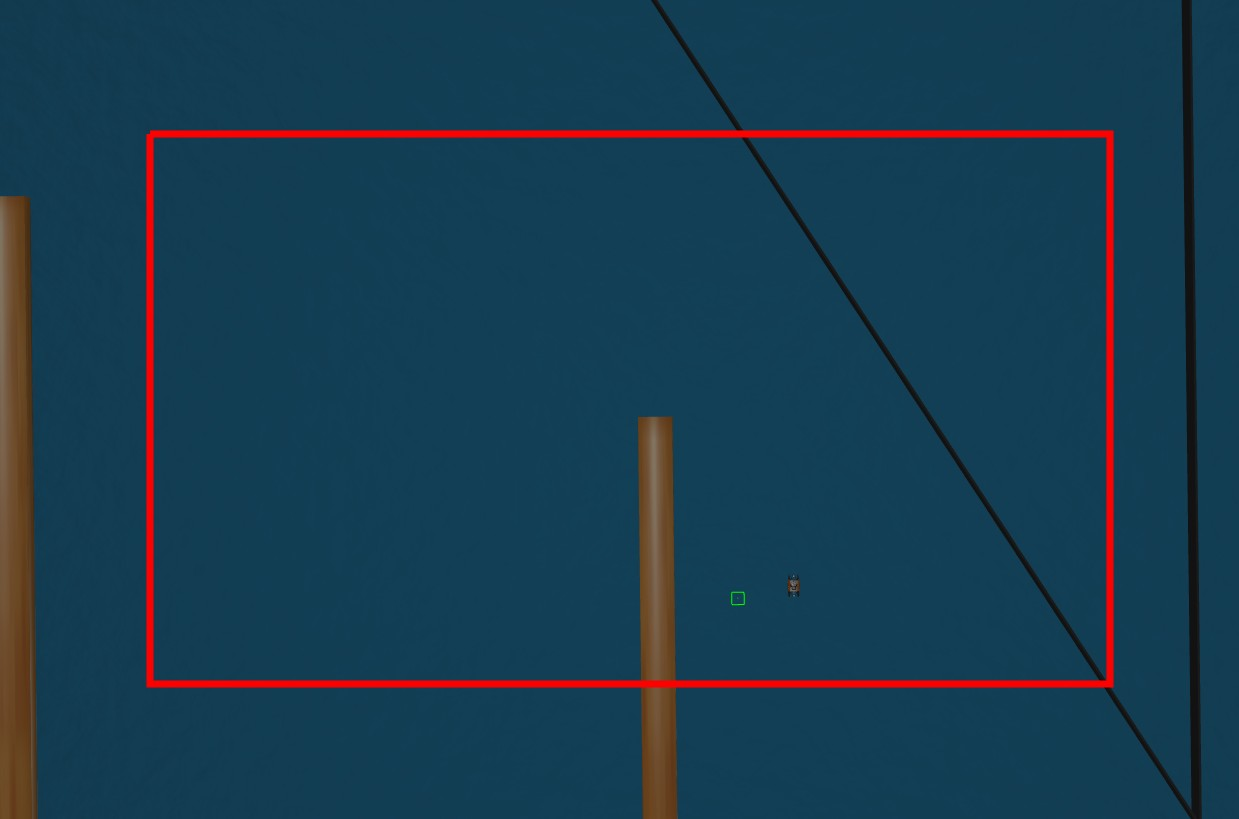
\includegraphics[width=0.7\textwidth]{fig/simulations/target_region_bm_1}
	\caption[The surrounding environment and target region for the first simulation.]{The surrounding environment and target region for the first simulation. The USV is depicted at its starting position.}
	\label{fig:target_region_bm_1}
\end{figure}

The following parameters were used in the simulations. The inflation radius is $r_i = \SI{3.0}{\meter}$, and cell sizes are $e_{cell} = \SI{1.0}{\meter}$. The turning radius of the simple Dubins paths is chosen as $\rho = \SI{0.5}{\meter}$. For the guidance law $\Delta_{max} = \SI{5.0}{\meter}$, $\Delta_{min} = \SI{2.0}{\meter}$, $K_\Delta = 1.0$, $U_{max} = \SI{1.5}{\meter/\second}$, $U_{min} = \SI{0.4}{\meter/\second}$, $y_{max} = \SI{5.0}{\meter}$, and $\chi_{max} = \pi/2$.

\figref{fig:bm1_alg_res} shows the result at the end of the simulation, when the USV has moved back to its starting position. \figref{fig:bm1_slam} shows the map and trajectory generated by SLAM at the end of the simulation. \figref{fig:bm1_res} shows the behavior of the method during the first simulation. At all times, data from the lidar is used to update the workspace partition and set cells as either free (blue) or blocked (red). This is why more and more cells of the partition appear in the visualization. Similarly, data from the simulated MBES is used to classify cells as covered (green). The partition does not represent the area beyond the edges of the target region, which is why cells are not updated (gray) in front of the USV in \figref{fig:bm1_res}c or to the left in \figref{fig:bm1_res}h. 

\begin{figure}[h!]
    \centering
	\makebox[\linewidth][c]{
	\begin{subfigure}[b]{0.5\textwidth}
		\centering
		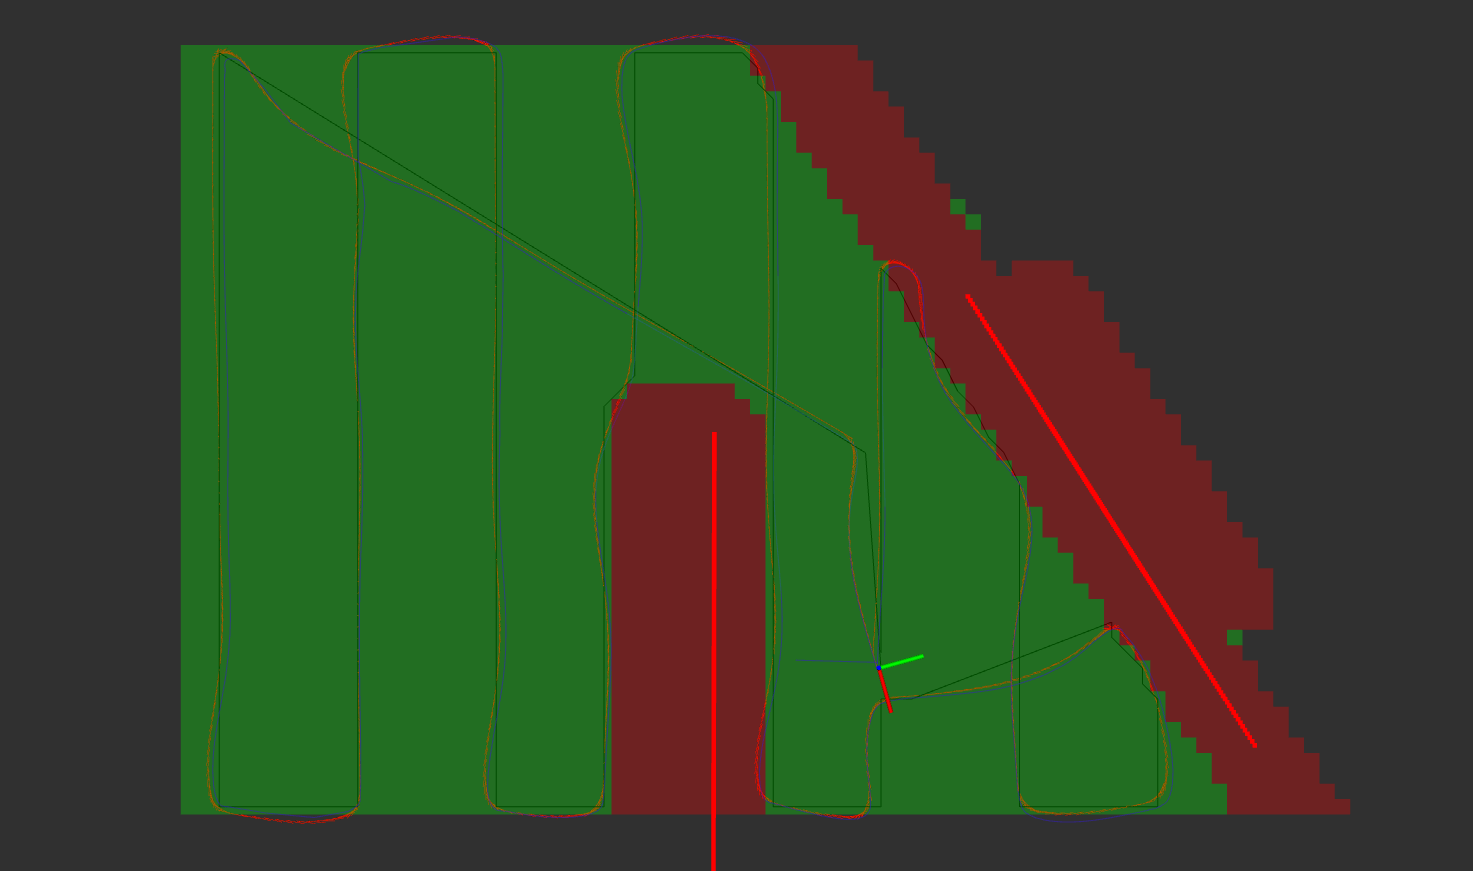
\includegraphics[width=1.0\textwidth,height=0.25\textheight]{fig/simulations/bm1_alg9}
		\caption{}
		\label{fig:bm1_alg_res}
	\end{subfigure}
	\begin{subfigure}[b]{0.5\textwidth}
		\centering
		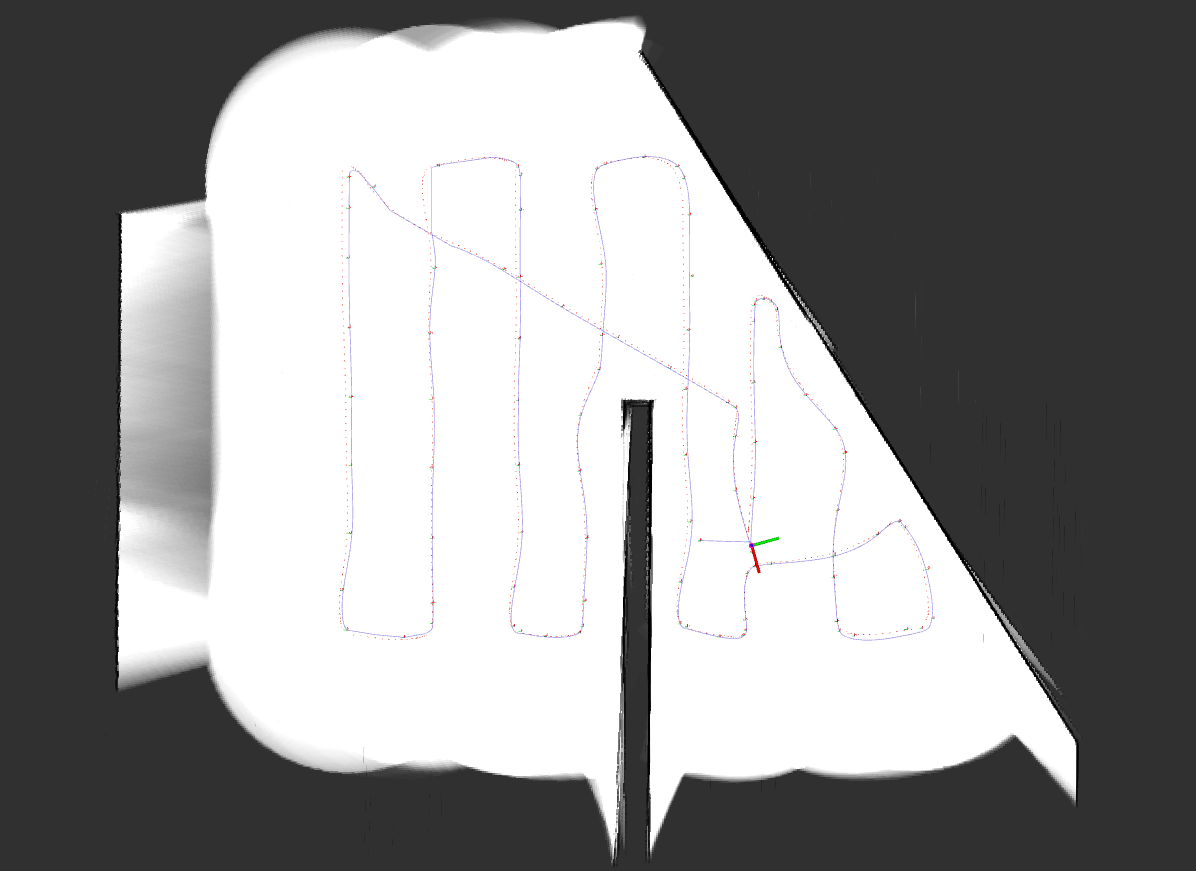
\includegraphics[width=1.0\textwidth,height=0.25\textheight]{fig/simulations/bm1_slam}
		\caption{}
		\label{fig:bm1_slam}
	\end{subfigure}
	}
	\caption[State at the end of the first simulation.]{State at the end of the first simulation. The red and blue curves are the ground truth and estimated trajectories, respectively. (a) Visualization by the system. Covered area is green, inflated obstacles are red, lidar detections are light-red. Black line is the connected waypoints. (b) Map and trajectory by SLAM. The white area of the map represents free space, the black area represents obstacles, and the dark gray area is unknown.}
	\label{fig:bm1_res_res}
\end{figure}

The subfigures of \figref{fig:bm1_res} show how the method reacted during the simulation. (a) In the beginning there is nothing in front of the USV, so the system starts by moving straight ahead. (b) When an obstacle appears in front of the USV, the system knows that there is free space to the right and therefore performs wall following. (c) The bottom of the target region is reached, and the system performs wall following of the virtual wall that is the edge of the target region. (d) A critical point is reached, so the system plans a path to the closest backtracking point. (e) The system reached the backtracking point and intelligently adjusted it a little to the left so that coverage overlap is reduced. Then it reached the bottom of the target region, figured out that the sweeping direction must be switched, and wall followed to the left. When turning back up, there is some coverage overlap because an obstacle blocks the USV from going further left. (f) After reaching the top of the region and coming back down, the system performs a little wall following in order to get to the side of the obstacle. (g) When coming back up the inter-lap spacing is chosen such that there are no uncovered cells left between the current and previous lap, even though some wall following occurred in the middle of the previous lap. (h) The remaining area of the target region is covered. 

% big figure --> decrease margins
\newgeometry{top=2cm,right=1.7in,left=1.7in,bottom=3cm}

\begin{figure}[h!]
    \centering
    \makebox[\linewidth][c]{
	\begin{subfigure}[b]{0.5\textwidth}
		\centering
		\includegraphics[height=0.20\textheight,width=1\textwidth]{fig/simulations/bm1_alg1_2}
		\caption{}
	\end{subfigure}
	\begin{subfigure}[b]{0.5\textwidth}
		\centering
		\includegraphics[height=0.20\textheight,width=1\textwidth]{fig/simulations/bm1_alg2_2}
		\caption{}
	\end{subfigure}
	}
	\makebox[\linewidth][c]{
	\begin{subfigure}[b]{0.5\textwidth}
		\centering
		\includegraphics[height=0.20\textheight,width=1\textwidth]{fig/simulations/bm1_alg3_2}
		\caption{}
	\end{subfigure}
	\begin{subfigure}[b]{0.5\textwidth}
		\centering
		\includegraphics[height=0.20\textheight,width=1\textwidth]{fig/simulations/bm1_alg4_2}
		\caption{}
	\end{subfigure}
	}
	\makebox[\linewidth][c]{
	\begin{subfigure}[b]{0.5\textwidth}
		\centering
		\includegraphics[height=0.20\textheight,width=1\textwidth]{fig/simulations/bm1_alg5_2}
		\caption{}
	\end{subfigure}
	\begin{subfigure}[b]{0.5\textwidth}
		\centering
		\includegraphics[height=0.20\textheight,width=1\textwidth]{fig/simulations/bm1_alg6_2}
		\caption{}
	\end{subfigure}
	}
	\makebox[\linewidth][c]{
	\begin{subfigure}[b]{0.5\textwidth}
		\centering
		\includegraphics[height=0.20\textheight,width=1\textwidth]{fig/simulations/bm1_alg7_2}
		\caption{}
	\end{subfigure}
	\begin{subfigure}[b]{0.5\textwidth}
		\centering
		\includegraphics[height=0.20\textheight,width=1\textwidth]{fig/simulations/bm1_alg8_4}
		\caption{}
	\end{subfigure}
	}
    \caption[Visualization of the boustrophedon motions method with constant coverage range at several stages during the simulation.]{Visualization of the boustrophedon motions method with constant coverage range at several stages during the simulation. The red-green-blue axis is the pose of the USV (z-axis positive upwards). Free covered area is represented by green, free uncovered area by blue, and inflated obstacles by red. The light-red dots are the current detection points of the lidar. The black line is the waypoints connected by line segments. The red curve trailing the USV is the ground truth trajectory, while the faint blue curve (often concealed by the red) is the estimated trajectory.}
	\label{fig:bm1_res}
\end{figure}

\FloatBarrier


\subsection{Varying coverage range}

\figref{fig:bm2_sim_env}a shows the target region and surrounding environment of this simulation. \figref{fig:bm2_sim_env}b shows the same region's depth. A simple linearly varying depth seabed which is at its deepest on the left, and at its shallowest on the right. More specifically, the coverage range varies from $\SI{14}{\meter}$ at the far left, to $\SI{4}{\meter}$ at the far right. All parameters of the system are the same as in the previous simulation.

\begin{figure}[h!]
    \centering
	\makebox[\linewidth][c]{
	\begin{subfigure}[b]{0.5\textwidth}
		\includegraphics[width=1.0\textwidth]{fig/simulations/target_region_bm_2}
		\caption{}
		\label{fig:bm2_tar_reg}
	\end{subfigure}
	\begin{subfigure}[b]{0.5\textwidth}
		\includegraphics[width=1.0\textwidth]{fig/simulations/bm2_depth.jpg}
		\caption{}
		\label{fig:bm2_depth}
	\end{subfigure}
	}
	\caption[The surrounding environment and target region for the second simulation.]{The second simulation. (a) The surrounding environment and target region. (b) The target region's varying depth seabed.}
	\label{fig:bm2_sim_env}
\end{figure} 

\figref{fig:bm2_alg} shows the result at the end of the simulation, and \figref{fig:bm2_slam} shows the map generated by SLAM at the end of the simulation. \figref{fig:bm2_res} shows the visualization by the system at several stages during the execution. 

\begin{figure}[h!]
    \centering
	\makebox[\linewidth][c]{
	\begin{subfigure}[b]{0.5\textwidth}
		\includegraphics[width=1.0\textwidth,height=0.2\textheight]{fig/simulations/bm2_alg_res}
		\caption{}
		\label{fig:bm2_alg}
	\end{subfigure}
	\begin{subfigure}[b]{0.5\textwidth}
		\includegraphics[width=1.0\textwidth,height=0.2\textheight]{fig/simulations/bm2_slam}
		\caption{}
		\label{fig:bm2_slam}
	\end{subfigure}
	}
	\caption[State at the end of the second simulation.]{State at the end of the second simulation. (a) Visualization by the system. Covered area is green and inflated obstacles are red. Black line is the connected waypoints. The blue curve is the estimated trajectory. (b) Map and trajectory by SLAM. The white area of the map represents free space, the black area represents obstacles, and the dark gray area is unknown.}
	\label{fig:bm2_alg_res}
\end{figure}

\restoregeometry 

\newgeometry{top=2.5cm,right=1.7in,left=1.7in,bottom=2.5cm}

\begin{figure}[h!]
    \centering
    \makebox[\linewidth][c]{
	\begin{subfigure}[b]{0.5\textwidth}
		\centering
		\includegraphics[height=0.20\textheight,width=1\textwidth]{fig/simulations/bm2_alg2}
		\caption{}
	\end{subfigure}
	\begin{subfigure}[b]{0.5\textwidth}
		\centering
		\includegraphics[height=0.20\textheight,width=1\textwidth]{fig/simulations/bm2_alg3}
		\caption{}
	\end{subfigure}
	}
	\makebox[\linewidth][c]{
	\begin{subfigure}[b]{0.5\textwidth}
		\centering
		\includegraphics[height=0.20\textheight,width=1\textwidth]{fig/simulations/bm2_alg4}
		\caption{}
	\end{subfigure}
	\begin{subfigure}[b]{0.5\textwidth}
		\centering
		\includegraphics[height=0.20\textheight,width=1\textwidth]{fig/simulations/bm2_alg5}
		\caption{}
	\end{subfigure}
	}
    \caption[Visualization of the boustrophedon motions method with varying coverage range at several stages during the simulation.]{Visualization of the boustrophedon motions method with varying coverage range at several stages during the simulation. The red-green-blue axis is the pose of the USV (z-axis positive upwards). Free covered area is green, free uncovered area is blue, and inflated obstacles are red. The light-red dots are current lidar detections. The black line is the connected waypoints. The blue curve is the estimated trajectory.}
	\label{fig:bm2_res}
\end{figure}




\section{Complete coverage maneuvering with bio-inspired neural network}

The bio-inspired neural network method was tested with the same target region and environment as in the previous simulation, i.e. the region shown in \figref{fig:bm2_tar_reg}. The parameters of the neural network model used in this simulation are $A = 50$, $B = 0.1$, $D = 0.1$, $\mu = 1$, and $E = 100$. The tuning parameter $\lambda$ is set to $\lambda = 0.1$ in order to prioritize areas that do not require a change of direction. The scaling factors $\lambda_i$ have all been set to $\lambda_i = 1$. The set of neighboring neurons is restricted by $r_0 = \sqrt{3}r_c$, meaning only the 6 surrounding circles in the partition are considered neighbors. The circles in the partition all have a radius of $r_c = \SI{5}{\meter}$. The rest of the parameters of the system are the same as in the first simulation described in Section \ref{sec:sim1}.

\figref{fig:binn_res} shows the visualization by the system at several stages during the execution, and \figref{fig:binn_slam} shows the map generated by SLAM at the end of the simulation. In \figref{fig:binn_res}, the next target cell is always the cell associated with the neuron that has the highest neural activity, but with a slight preference for going straight forward.



\begin{figure}[h!]
    \centering
    \makebox[\linewidth][c]{
	\begin{subfigure}[b]{0.5\textwidth}
		\centering
		\includegraphics[height=0.20\textheight,width=1\textwidth]{fig/simulations/binn_alg1}
		\caption{}
	\end{subfigure}
	\begin{subfigure}[b]{0.5\textwidth}
		\centering
		\includegraphics[height=0.20\textheight,width=1\textwidth]{fig/simulations/binn_alg3}
		\caption{}
	\end{subfigure}
	}
	\makebox[\linewidth][c]{
	\begin{subfigure}[b]{0.5\textwidth}
		\centering
		\includegraphics[height=0.20\textheight,width=1\textwidth]{fig/simulations/binn_alg4}
		\caption{}
	\end{subfigure}
	\begin{subfigure}[b]{0.5\textwidth}
		\centering
		\includegraphics[height=0.20\textheight,width=1\textwidth]{fig/simulations/binn_alg5}
		\caption{}
	\end{subfigure}
	}
	\caption[Visualization of the bio-inspired neural network method at several stages during the simulation.]{Visualization of the bio-inspired neural network method at several stages during the simulation. The red-green-blue axis is the pose of the USV (z-axis positive upwards). Free covered area is green, free uncovered area is blue, and inflated obstacles are red. The light-red dots are current lidar detections. The blue curve is the estimated trajectory. The green curve is the currently followed simple Dubins path.}
	\label{fig:binn_res}
\end{figure}

\begin{figure}[h!]
	\centering
	\includegraphics[width=0.7\textwidth]{fig/simulations/binn_slam}
	\caption[Map by SLAM at the end of the third simulation.]{Map by SLAM at the end of the third simulation. The white area of the map represents free space, the black area represents obstacles, and the dark gray area is unknown.}
	\label{fig:binn_slam}
\end{figure}

\restoregeometry 


\section{Discussion}

\subsection{Sensor fusion and SLAM}

The SLAM map generated in \figref{fig:sim_sensor_fusion} quite accurately depicts the simulated environment. The walls are straight, there is a clear transition between obstacles and free space, and the proportions look very reasonable. Because of the lidar's restricted range of only 25 m, the SLAM system is never able to see across the middle, and thus this area remains uncertain. In the top left corner, there is an opening without any walls. Even though the USV traveled across this area, the area still remains uncertain in the map. It could be reasoned that everything within the lidar's range should be considered free space when there are no detections. However, since a lidar's range varies depending on the reflectivity of the material and lighting conditions, care must be taken when assuming free space in the case of no detections. Cartographer has a parameter allowing to set the distance for assumed free space. In this case, the purpose was to create an accurate map, so there was no reason to assume free space.

\figref{fig:bm1_slam} shows the SLAM map, estimated trajectory, and ground truth trajectory for the first simulation. The SLAM map accurately depicts the target region in \figref{fig:target_region_bm_1}. Looking closely at the map, there have been some small errors, as evident by the short strips of duplicated walls on the right-most inclined wall. This is caused by the SLAM system thinking for a short time that it has a different pose than it really has, and then mapping the environment at the wrong place. In a carefully tuned system, such errors should rarely be seen. There are also some inaccuracies in the mapping of the jetty in the middle of the map. Overall, however, the mapping looks good. The estimated trajectory also approximates the ground truth well. It can be seen to drift a little at times, but it always corrects itself.

The results of the second and third simulations in \figref{fig:bm2_slam} and \figref{fig:binn_slam} show many of the same properties. These maps both depict the environment of \figref{fig:bm2_tar_reg}. It should be noted, however, that the bio-inspired neural network method used to create the map in \figref{fig:binn_slam} results in more errors in the map. This is likely because this method causes the USV to turn more, which is more difficult for accurate pose estimation. In particular, turns performed when the lidar detects nothing, i.e. when the USV is far from obstacles, prevents corrections to pose estimations by loop closure. The map can only be corrected with loop closures after the lidar starts detecting obstacles again. If no distinct features are then detected, the accumulated errors in localization might be too big and difficult to correct for. 

This last argument highlights another very important issue for this particular application. Namely, that the range of the lidar is very short compared to the size of the workspace. This means the lidar scans are often empty or consist of only a single line-segment of detection points representing the closest wall or jetty. Cartographer is mainly a lidar-based SLAM method, and relies heavily on these lidar scans. The data from the lidar, however, is by itself not nearly enough information to perform SLAM. As a result, the sensor fusion and SLAM system is very dependent on GNSS, even when close to obstacles. 


\subsection{CCPP with boustrophedon motions}


The first simulation is summarized in \figref{fig:bm1_res_res}. \figref{fig:bm1_alg_res} shows that complete coverage is achieved, and upon completion the USV travels back to the starting point and stops there. This is also a great example of how the line-of-sight smoothing of A* paths works as intended. The subfigures of \figref{fig:bm1_res} also verify that the many autonomous subfunctions of the implemented system work as intended in a simulated environment. The localization and map in \figref{fig:bm1_slam} provided by the sensor fusion and SLAM subsystem has also proved to be good enough for the algorithms in the rest of the system to function properly and achieve complete coverage.

The second simulation, in \figref{fig:bm2_alg} and \figref{fig:bm2_res}, shows how the method performed with a simple linearly varying sea depth. The seabed shown in \figref{fig:bm2_depth} is overly simplistic, but the simulation nonetheless showcases the method's ability to react to the varying coverage range of the MBES. 
\figref{fig:bm2_res} shows the coverage range shrinking as the USV moves farther to the right and towards shallower waters. As expected, the inter-lap spacing shrinks to accommodate the smaller coverage range while still avoiding overlapping coverage.

Note that the second simulation shows a very idealistic scenario, where the coverage range is constant along the entire length of one lap. Realistically, even with the best possible sweeping direction, there will be some difference between the shallowest and deepest point in one lap, which will necessarily result in some overlapping coverage. Since the implemented method simply chooses the sweeping direction as the heading angle the system starts with, the choice of sweeping direction is left entirely in the hands of the operator. Leaving this important part of the survey to chance, or to depend on the operator's prior knowledge of the area, is a weakness of the system. A possible extension is therefore to incorporate the ideas of \citet{galceran2012efficient} for choosing the best sweeping direction, although it would have to be done online without any prior knowledge. As suggested in the same paper, a further improvement would be segmentation of the target region into several smaller similar-depth target regions. This would also have to be done online. Developing online algorithms for these two extensions would be a great step forward in the field of autonomous seabed mapping, and would result in a system that incorporates many of the best practices of hydrographic surveying.

\subsection{CCPP with bio-inspired neural network}

The result of running the third simulation with the bio-inspired neural network is shown in \figref{fig:binn_res}. The neural network is set up to always target the neighboring circle with the highest neural activity, but with a preference for reducing turns. As seen in subfigures (a) and (b), this tends to create spiraling patterns. Once the spiral pattern is complete, the remaining uncovered circles are the only cells with high neural activity. Consequently, the system is attracted to these last remaining uncovered cells, as seen in (c) and (d), and achieves complete coverage.

This method tends to create more turns than the boustrophedon motions method, even though the target cell is chosen with a preference for less turning. In the end, this preference actually causes more turns in total. The method ends up always delaying turns to the last possible moment, which is generally not an intelligent way to cover an area with the circular partition used here. Turning reduces not only the accuracy of SLAM as discussed above, but more importantly it reduces the quality of the bathymetric data acquired by the MBES. This is because during turning the accuracy of pose estimation is reduced, which introduces errors in the mapping of the seabed. More turns also increase the duration and fuel consumption of the survey. 

It should be noted that some other works in the literature have achieved somewhat better results with almost the same method (e.g. \citet{Scibilia2012} and \citet{luo2008bioinspired}), and it is likely because of different tuning parameters resulting in a more intelligent path. The performance of the method might see a slight improvement by altering the behavior of the neural network and the choice of the target neuron. For instance by modifying equation \eqref{eq:binn_pos} or choosing the tuning parameter $\lambda_i$ wisely. \citet{Scibilia2012} states for instance that $\lambda_i$ is used to prioritize areas closer to the initial AUV position. The results of \citet{luo2008bioinspired} show paths that look very much like boustrophedon motions. However, they use a square cell partition which, based on these results, might be better suited.

The partition used for this method is not able to adapt to a varying coverage range. Instead, the size of the circular cells must be determined based on the shallowest point in the target region, i.e. the point which results in the minimum coverage range. Doing this ensures complete coverage, but may result in a lot of overlapping coverage if the depth varies a lot. A possible solution to this would be to repartition the target region with another cell size when the depth varies more than some threshold. Alternatively, the target region could be divided into several similar-depth subregions, each with a different cell size depending on the shallowest point within the subregion.

Another drawback of the circular cell partitioning is that the cell size determined by the water depth, also determines how accurately obstacles are represented. In this simulation, the cells have a radius of $r_c = \SI{5.0}{\meter}$ in order to represent the coverage range. This means that an area of free space up to $\SI{20.0}{\meter}$ wide may be considered an obstacle with an unfortunate placement of the circles. By comparing the resulting coverage of \figref{fig:bm2_alg} and \figref{fig:binn_res}d, it is clear that the circular partition does a worse job of representing obstacles. The square cell partitioning avoids these issues by separating the coverage range from the cell size, and allowing multiple cells to be marked as covered together. An obvious further development of the bio-inspired neural network CCPP method would therefore be to incorporate the square cell partitioning instead.

\subsection{Path following}

\figref{fig:bm1_alg_res} shows that the ground truth trajectory (red line) manages to track the waypoints (black line) well. Keep in mind that the path that is actually followed is not the black line connecting the waypoints, but a simple Dubins path generated from the USV's pose to the newest waypoint. This means that the overshoot that appears around sharp corners such as in \figref{fig:bm1_res}b is to be expected, because the generated simple Dubins path accounts for the turning radius. This also means that the planned simple Dubins path often goes outside the green and blue region classified as free space in the partition, and into the red region classified as inflated obstacles. As long as obstacles are inflated with a radius greater than the maximum USV footprint plus the turning radius, i.e. $r_i > r_{max} + \rho$, the USV will avoid collision. However, this should be done more intelligently, because the increased obstacle inflation radius means that the coverage of the seabed close to or beneath obstacles is reduced. Consider the possibility of inflating obstacles in two steps instead, first to incorporate the USV footprint and then secondly to incorporate the turning radius. This would make it possible to separate the obstacles region into two new regions: a region which specifies when the USV has to start turning, and when the USV would definitely be in collision.

The USV manages to follow the path in the second and third simulation as well, see \figref{fig:bm2_alg} and \figref{fig:binn_res}. Looking more closely at \figref{fig:bm2_alg}, the USV often overshoots a little after the turns. This can likely be improved by a finer tuning that has a little less aggressive steering. For example, by increasing the minimum lookahead distance $\Delta_{min}$ or reducing the convergence rate $K_\Delta$. In \figref{fig:binn_res}, the actual simple Dubins paths to be followed are shown in green. The USV deviates slightly from the path, always on the outer side of the turn. This likely means the turning radius is too small for the simulated model. Another contributing factor could be that the implemented low-level controllers for the simulated USV are very simple and not finely tuned.

Another thing to note about the results, is that the pose and trajectory of the USV is provided by SLAM, and the SLAM system will adjust the pose and trajectory if it discovers it has done an error. The pose adjustments can interfere with the path following by causing steps in the pose of the USV. Similarly, the trajectory adjustments can make it seem like the path following was better or worse than it actually was, since the waypoints are not adjusted.

\chapter{Experiments}

\section{Experimental setup}

The developed system has been implemented and tested on the Otter USV in the harbor of Trondheim. The testing area contains various obstacles like boats and jetties, and is shown in \figref{fig:testing-arena}. Since the boustrophedon motions CCPP method performed best in the simulations, only that method has been tested experimentally.

\begin{figure}[h!]
    \centering
	\makebox[\linewidth][c]{
	\begin{subfigure}[b]{0.5\textwidth}
		\includegraphics[width=1.0\textwidth]{fig/results/testing-arena2}
		\caption{Top-down view from Google Maps.}
	\end{subfigure}
	\begin{subfigure}[b]{0.5\textwidth}
		\includegraphics[width=1.0\textwidth]{fig/results/testing-arena-real}
		\caption{Picture on the testing day.}
	\end{subfigure}
	}
	\caption{The testing area used for the Otter USV.}
	\label{fig:testing-arena}
\end{figure}

The Otter USV has not been equipped with a multibeam echosounder during the experiments.  A symmetric constant coverage range is assumed for the MBES instead. Consequently, variable water depth is not considered during path planning. This means the system will be performing almost the same maneuvers as in a real bathymetric survey, but with a simulated MBES that reports a constant depth.

\section{Complete coverage maneuvering with boustrophedon motions}

\subsection{First experiment}

The boustrophedon motions CCPP method was first tested with a symmetric constant coverage range of $\SI{16}{\meter}$, i.e. the USV was assumed to cover $\SI{8}{\meter}$ of the seabed in both port and starboard directions. 

The following parameters were used in the experiment. The inflation radius is $r_i = \SI{5.0}{\meter}$, and cell sizes are $e_{cell} = \SI{1.0}{\meter}$. The turning radius of the simple Dubins paths is chosen as $\rho = \SI{1.0}{\meter}$. For the guidance law $\Delta_{max} = \SI{4.0}{\meter}$, $\Delta_{min} = \SI{1.5}{\meter}$, $K_\Delta = 1.0$, $U_{max} = \SI{1.0}{\meter/\second}$, $U_{min} = \SI{0.4}{\meter/\second}$, $y_{max} = \SI{5.0}{\meter}$, and $\chi_{max} = \pi/2$.

The resulting trajectory reported by the GNSS receiver is illustrated in \figref{fig:res2_gnss} (not actual location of boats on the testing day). \figref{fig:res2_slam} depicts the same trajectory and a map of the surroundings generated by Cartographer. \figref{fig:res2} shows the visualization by the system at several stages during the experiment. The USV reaches the right edge of the target region, which is why the visualization does not expand further right. The operator had to intervene at the end in \figref{fig:res2}d, because the USV was headed straight for an obstacle. A video demonstrating this experiment is available at \url{https://youtu.be/hqOUKtosnFw} and in the electronic attachment of this thesis.

\begin{figure}[h!]
    \centering
	\makebox[\linewidth][c]{
	\begin{subfigure}[t]{0.5\textwidth}
		\centering
		\includegraphics[width=1.0\textwidth]{fig/results/gnss_1.jpg}
		\caption{}
		\label{fig:res2_gnss}
	\end{subfigure}
	\begin{subfigure}[t]{0.5\textwidth}
		\centering
		\includegraphics[width=1.0\textwidth]{fig/results/res2_slam_2.jpg}
		\caption{}
		\label{fig:res2_slam}
	\end{subfigure}
	}
	\caption[State at the end of the first experiment.]{State at the end of the first experiment. The starting position was at the left end of the trajectories. (a) GNSS trajectory overlaid an aerial photo. (b) Trajectory and map by SLAM. The white area of the map represents free space, the black area represents obstacles, and the gray area is unknown. Transparent colors mean uncertainty.}
	\label{fig:res2_trajectory}
\end{figure} 

\begin{figure}[h!]
    \centering
    \makebox[\linewidth][c]{
	\begin{subfigure}[b]{0.5\textwidth}
		\centering
		\includegraphics[height=0.25\textheight,width=1\textwidth]{fig/results/ex1_alg1}
		\caption{}
	\end{subfigure}
	\begin{subfigure}[b]{0.5\textwidth}
		\centering
		\includegraphics[height=0.25\textheight,width=1\textwidth]{fig/results/ex1_alg2}
		\caption{}
	\end{subfigure}
	}
	\makebox[\linewidth][c]{
	\begin{subfigure}[b]{0.5\textwidth}
		\centering
		\includegraphics[height=0.25\textheight,width=1\textwidth]{fig/results/ex1_alg3}
		\caption{}
	\end{subfigure}
	\begin{subfigure}[b]{0.5\textwidth}
		\centering
		\includegraphics[height=0.25\textheight,width=1\textwidth]{fig/results/ex1_alg4}
		\caption{}
	\end{subfigure}
	}
\caption[Visualization of the boustrophedon motions method at several stages during the first experiment]{Visualization of the boustrophedon motions method at several stages during the first experiment. The red-green-blue axis is the pose of the USV (z-axis positive upwards). Free covered area is green, free uncovered area is blue, and inflated obstacles are red. The light-red dots are current lidar detections. The black line is the connected waypoints. The blue curve is the estimated trajectory.}
	\label{fig:res2}
\end{figure}

\FloatBarrier

\subsection{Second experiment}

The second experiment consisted of the same setup as in the first experiment with the same system parameters. The resulting trajectory according to the GNSS receiver is shown in \figref{fig:gnss_test2}. \figref{fig:ex2_slam} shows the SLAM map and estimated trajectory at different stages during the experiment. \figref{fig:ex2_res} shows the visualization by the system during different stages of the experiment. The USV reaches the right edge of the target region in \figref{fig:ex2_res}b, which is why the visualization does not expand further right. The experiment was aborted at the end because the system's estimated position deviated too much from the observed position.

\newgeometry{top=2.5cm,right=1.7in,left=1.7in,bottom=2.5cm}

\begin{figure}[h!]
	\centering
	\includegraphics[height=0.3\textheight]{fig/results/gnss_3.jpg}
	\caption{GNSS trajectory in the second experiment.}
	\label{fig:gnss_test2}
\end{figure}

\begin{figure}[h!]
    \centering
    \makebox[\linewidth][c]{
	\begin{subfigure}[b]{0.5\textwidth}
		\centering
		\includegraphics[width=1\textwidth]{fig/results/ex2_slam_1}
		\caption{}
	\end{subfigure}
	\begin{subfigure}[b]{0.5\textwidth}
		\centering
		\includegraphics[width=1\textwidth]{fig/results/ex2_slam_2}
		\caption{}
	\end{subfigure}
	}
	\makebox[\linewidth][c]{
	\begin{subfigure}[b]{0.5\textwidth}
		\centering
		\includegraphics[width=1\textwidth]{fig/results/ex2_slam_nice}
		\caption{}
	\end{subfigure}
	\begin{subfigure}[b]{0.5\textwidth}
		\centering
		\includegraphics[width=1\textwidth]{fig/results/ex2_slam_nice2}
		\caption{}
	\end{subfigure}
	}
\caption[Trajectory and map according to the SLAM system Cartographer at different stages of the second experiment.]{Trajectory and map according to the SLAM system Cartographer at different stages of the second experiment. The white area of the map represents free space, the black area represents obstacles, and the gray area is unknown. Transparent colors mean uncertainty.}
	\label{fig:ex2_slam}
\end{figure}

\begin{figure}[h!]
    \centering
    \makebox[\linewidth][c]{
	\begin{subfigure}[b]{0.5\textwidth}
		\centering
		\includegraphics[height=0.25\textheight,width=1\textwidth]{fig/results/ex2_alg3}
		\caption{}
	\end{subfigure}
	\begin{subfigure}[b]{0.5\textwidth}
		\centering
		\includegraphics[height=0.25\textheight,width=1\textwidth]{fig/results/ex2_alg7}
		\caption{}
	\end{subfigure}
	}
		\makebox[\linewidth][c]{
	\begin{subfigure}[b]{0.5\textwidth}
		\centering
		\includegraphics[height=0.25\textheight,width=1\textwidth]{fig/results/ex2_alg_1}
		\caption{}
	\end{subfigure}
	\begin{subfigure}[b]{0.5\textwidth}
		\centering
		\includegraphics[height=0.25\textheight,width=1\textwidth]{fig/results/ex2_alg9}
		\caption{}
	\end{subfigure}
	}
	\makebox[\linewidth][c]{
	\begin{subfigure}[b]{0.5\textwidth}
		\centering
		\includegraphics[height=0.25\textheight,width=1\textwidth]{fig/results/ex2_alg11}
		\caption{}
	\end{subfigure}
	\begin{subfigure}[b]{0.5\textwidth}
		\centering
		\includegraphics[height=0.25\textheight,width=1\textwidth]{fig/results/ex2_alg_2}
		\caption{}
	\end{subfigure}
	}
\caption[Visualization of the boustrophedon motions method at several stages during the second experiment]{Visualization of the boustrophedon motions method at several stages during the second experiment. The red-green-blue axis is the pose of the USV (z-axis positive upwards). Free covered area is green, free uncovered area is blue, and inflated obstacles are red. The light-red dots are current lidar detections. The black line is the connected waypoints. The blue curve is the estimated trajectory.}
	\label{fig:ex2_res}
\end{figure}

\restoregeometry

\FloatBarrier

\section{Discussion}

\subsection{Sensor fusion and SLAM}

\figref{fig:res2_slam} shows the map and trajectory estimated by SLAM for the first experiment. Comparing it to the aerial photo and the GNSS trajectory in \figref{fig:res2_gnss}, there are several signs of drift and deviation in the map. Boats at the top and bottom of the map are not really recognizable as boats, and the jetty at the bottom is drawn twice with a different angle and position. The cause for this is that the SLAM system struggles to accurately localize itself, and so multiple things are mapped on top of each other, resulting in the cluttered map seen in the figure. The top and bottom jetties are also shifted a little sideways compared to each other, so the paths that appear perpendicular to the jetties in the aerial photo, appear sloped in the SLAM map.

 On the other hand, the SLAM trajectory seems to approximate the GNSS trajectory very well, which might mean that there are some inconsistencies in the transformations between the lidar and IMU. However, that does not explain what happens to the mapping of the boats in the top left corner of the SLAM map. Those errors are more likely caused by a drift in the orientation. In fact, during the experiment when the USV moved straight forward, the estimated position was seen to move at an angle compared to the heading (this can be seen at some times in the attached video). This strongly suggest a consistent offset between the estimated orientation and the real orientation. Keep in mind that the GNSS trajectory does not necessarily depict the actual ground truth (it has the standard GNSS accuracy), but it is the closest thing available and will therefore be treated as a ground truth in the discussion.

%Exactly why the SLAM system struggled is hard to pinpoint, but several factors were observed during the experiments.
There are also other factors that were observed to affect the SLAM system during the experiment. The mounted lidar states a range of $\SI{25}{\meter}$, which will be somewhat reduced in outdoor operation. However, in the experiments, the lidar never detected anything more than about $\SI{14}{\meter}$ away. Furthermore, this was only when the lidar rays hit the obstacle's surface at a right angle. When the lidar rays hit the surface with an angle, the range was observed to drop much lower. Dark objects, because of their low reflectivity, were the most difficult to detect. Some objects, like ships with a black hull, were not detected at all. The single scan plane of the lidar also caused some trouble. The lidar was mounted relatively high on the USV, so the jetty at the top of the SLAM map was too low to be seen when the USV moved towards the jetty. Luckily, there was a detectable boat on the other side of the too low jetty that prevented the USV from crashing. Because the USV has a small pitch angle when moving forward, the jetty was seen when moving away and appears in the SLAM map. 

In the second experiment, the mapping of the same area is better, as seen in \figref{fig:ex2_slam}a. The top and bottom jetty is still shifted a little sideways compared to each other, causing the almost perpendicular laps of \figref{fig:gnss_test2} to appear slightly sloped in the SLAM map. In \figref{fig:ex2_slam}b, the SLAM system failed to recognize the bottom jetty when backtracking to the left, which once again seems to have been caused by a drift in orientation. No system parameters were changed between the two experiments, so it is a bit unclear as to why this SLAM map is better. The weather did change though, becoming a little sunnier. This caused a lot of false detections in the lidar, which is not clear from the SLAM map because only persistent detections appear in the map. However, the instantaneous data from the lidar used in the rolling window was affected. This had an impact on path planning which is discussed in the next section.

In \figref{fig:ex2_slam}b the SLAM system has gone a long time without any lidar detections, and the map becomes very uncertain because of it (transparent white in the figure). The lack of lidar detections means the SLAM system must depend entirely on GNSS and IMU for localization. This should cause no trouble if the fusing of GNSS and IMU data is good. However, the current pose and recent trajectory of the USV in \figref{fig:ex2_slam}b deviates a lot from the GNSS trajectory in \figref{fig:gnss_test2}. In \figref{fig:ex2_slam}c, only a couple of seconds later, Cartographer actually realizes this and corrects for it. Note that this means the fused GNSS and IMU data must have been available all the time, but is only incorporated correctly after the lidar starts detecting obstacles again. This most likely means that the implementation of Cartographer runs some of its graph optimizations only after it has received a certain number of lidar detections.
The documentation states that "the optimization is run in batches once a certain number of trajectory nodes was inserted" \citep{website:CartographerRos}. Based on the obtained results, the generation of these trajectory nodes likely requires lidar detections. This makes the proposed setup in Cartographer very poorly suited for open marine environments, especially when using a short range lidar. Exactly the same thing happens once more in the experiment, and can be seen in \figref{fig:ex2_slam}d. After that, the experiment was aborted. The fact that the USV drifts in the same direction both times, further emphasizes the possibility of an error in the orientation estimation.

\subsection{CCPP with boustrophedon motions}

The GNSS trajectory of the first experiment is shown in \figref{fig:res2_gnss}, and it clearly depicts a  boustrophedon motion between the jetties. \figref{fig:res2} shows that the system also manages to achieve complete coverage for this area. Obstacles are identified correctly by the system, and the CCPP method successfully plans a collision-free path that steers clear of them. The planned path can be seen inside the inflated obstacles region at some places, or further into the free space region than it should be. This is because the status of the cells has changed after the USV reached those waypoints. The large inaccuracies in localization and mapping experienced during this test makes this very noticeable.

At the very end of the experiment, just after \figref{fig:res2}d, the system ended up planning a backtracking path straight through the obstacles seen at the bottom. This was caused by an error in the implementation of the system that incorrectly dealt with multiple status changes in a cell, e.g. caused by mapping inaccuracies. This was discovered and fixed before the second experiment. However, it does illustrate the fact that the CCPP method contains very little logic for dealing with uncertainties. Currently, the only logic aimed at this is the fact that the system replans the next waypoint if it becomes blocked.

The results of the second experiment are largely influenced by false lidar detections due to sunlight, and localization drift. The GNSS trajectory in \figref{fig:gnss_test2} shows that the USV first covers the area between the jetties with a single boustrophedon motion. The laps are not as nice and straight as in the previous experiment, but this is because the system avoids the non-existing obstacles reported by false lidar detections. Next, the system backtracks and starts a new boustrophedon motion. This motion suffers from two detours. The cause of the detours was, as explained in the last section, due to localization drift. After the second detour the experiment is aborted.  Even though the resulting trajectory is not as good as in the simulations, it does show the system's main properties working in a real-world environment. Namely, boustrophedon motions and backtracking.

The subfigures of \figref{fig:ex2_res} show a closer look at how the CCPP method reacted during the second experiment. In \figref{fig:ex2_res}a, a false detection appears in front of the USV. Since it is so close to the USV, this false detection causes the USV to wall follow to the side of it. Note that it is not just a single false detection that causes this, but several. They appear, the obstacle is inflated, the path is replanned, and then they disappear. The turn at the very beginning of the boustrophedon motion, in the lower left corner, was not caused by false detections. This was due to the USV's starting position being inside the inflated obstacles region. This is a situation that is not explicitly considered in the implemented system, but since the system planned a path anyway, it is not entirely safe.

For the rest of the subfigures in \figref{fig:ex2_res}: (b) After wall following to the side of the false obstacle in (a) and of another one on the way down, there are two small uncovered regions remaining within the covered area. A possible extension of the system would therefore be to wall follow not just to the side of obstacles, but around them. This would have covered these remaining areas. (c) The USV backtracks and begins another boustrophedon motion to the left of the starting point (the method was slightly altered for this experiment to ignore the closer but very small enclosed uncovered areas). The sweeping direction is switched because of a false detection. (d) Since the sweeping direction was switched, the USV now continues back down on the left. (e) The jump in the position of the SLAM system moves the USV far out from the desired path. (f) The USV manages to get back on the path after the jump in position. A new jump appears, and the same thing happens. When the localization drifts as much as it did in this experiment, the coverage reported by the system is not correct anymore. After loop closures and trajectory adjustments, the coverage should ideally be recalculated based on the new estimated trajectory. In this experiment, however, even the trajectory with loop closure at the end had significant uncorrected drift which would later have caused problems.

\subsection{Path following}

The localization in both experiments is not really sufficient for making accurate conclusions about the performance of the path following method. The estimated trajectory is adjusted several times during the experiment by the SLAM system, while the planned path is kept still throughout the whole experiment. Furthermore, it should be kept in mind that the planned path in all figures are the waypoints connected by line segments, and not the actual simple Dubins paths followed.

Even with the poor localization, the USV still managed to track the paths. In \figref{fig:res2}, the estimated trajectory seems to follow the planned path reasonably well most of the time. The same is true for \figref{fig:ex2_res}. The path following method has therefore been proved to be robust, and should be considered satisfactorily in both experiments. There are significant deviations several places, but it is hard to tell whether they are because of the path following, localization, or both. However, the path following is definitely to blame for some of it. In the first experiment, there are some oscillations in the third lap, see \figref{fig:res2}c. This may seem to be because of bad path following, but it is clear from looking at logged data of the experiment that these oscillations are largely affected by pose adjustments of the SLAM system (it can also be seen from the attached video).

All these problems with localization also made it very hard to tune the parameters of the system. A significant performance increase in path following is therefore likely achievable by better tuning of the system. One thing that managed to make the system very reliable and safe during the experiments, was the buffer safety zone that is added around all obstacles. This allowed for many smaller things to go wrong, while still making sure the complete system functioned as a whole and avoided collisions.


\chapter{Concluding remarks}

\section{Conclusions}

%SLAM: Error in orientation estimation. Current Cartographer setup cannot handle going without lidar detections. Some better tuning required, pose adjustments interfered with path planning and path following.

In this thesis, an autonomous online complete coverage maneuvering system for USVs has been designed, implemented, and tested. The system is intended for use in seabed mapping, and one of the main contributions of this work is a novel approach to online CCPP for variable coverage range sensors. Implementations in ROS are provided as open source packages. 

An approach to sensor fusion with the SLAM system Cartographer has been proposed. Sensor data from lidar, IMU and GNSS are used.
Experiments revealed what is likely a small error in the incorporation of the orientation from the IMU, which reduced the performance of SLAM. The experiments also revealed that the presented configuration of Cartographer is unable to accurately perform localization with only GNSS and IMU in cases where the lidar cannot detect anything. This makes the approach poorly suited for open marine environments and the use of a short range lidar. It is therefore recommended to use another approach that incorporates GNSS data in a better way, and that does not require detecting something with the lidar at all times.

It has been shown that the low-cost 2D lidar used in the experiments is, by itself, not good enough for reliable obstacle detection in marine environments. Sunlight produces false detections, and some dark objects, such as boats with a black hull, were not detected at all. The range was barely sufficient, and the single horizontal scan plane caused some obstacles to go undetected. It is therefore recommended to make use of additional low-cost sensors like cameras or proximity sensors to ensure more obstacles are detected. Measures must also be taken to reduce false detections of the lidar.

A map processing technique for inflating obstacles has been presented, and shown to work well in both simulations and experiments. Two workspace partitioning methods make use of the processed map. Circular cell partitioning has been presented and simulated with unsatisfactorily results. A square cell partitioning for use with variable coverage range sensors has been proposed and shown to perform well in both simulations and experiments.

Two CCPP methods have also been presented. A method based on BINN yielded inefficient paths in simulations, but has proved potential in other works of the literature. The proposed boustrophedon motions method performed well in both simulations and experiments, and shows great potential for real-world applications. Further development to increase the method's robustness, especially towards inaccuracies, is recommended.

An approach to ensure feasible paths is also presented, which together with an LOS guidance law perform path-following control of the USV. The USV managed to track the paths well in simulations, but resulted in some larger deviations in the experiments. The performance was still good, but poor localization in the experiments makes accurate conclusions about the performance hard. 

The complete system has been tested in both simulations and real-world experiments with the Otter USV. The system performed well in simulations, and was shown to efficiently achieve complete coverage of completely unknown static environments. In real-world experiments, localization and mapping suffered from inaccuracies, but the rest of the system performed satisfactorily, including the proposed methods for CCPP, feasible path generation and path following. 

In conclusion, the proposed system performed satisfactorily and achieved complete coverage in simulations, and in real-world experiments under certain conditions. However, the sensor fusion and SLAM system did not perform satisfactorily in real-world experiments and should be improved.

\section{Further work}

The proposed system's ability to handle a varying coverage range has only been verified in simulations. Further testing of the system should include experimental testing with a multibeam echosounder in a variable depth environment. Testing in dynamic environments with moving obstacles is also left undone. For increased safety, the system should be improved to be able to discern between moving and stationary obstacles. In particular, the system should be in compliance with the Convention on the International Regulations for Preventing Collisions at Sea (COLREGs).

Further development should aim to increase the efficiency of the complete coverage paths even more. This could, for instance, be done by incorporating the ideas of \citet{galceran2012efficient} for choosing the best sweeping direction, although it would have to be done online without any prior knowledge. As suggested in the same paper, another improvement would be segmentation of the target region into several smaller similar-depth regions. This would also have to be done online. Implementing these extensions would result in an autonomous system that incorporates many of the best practices of hydrographic surveying.

Further development of the system will also require the improvement of the sensor fusion and SLAM system. Additional low-cost sensors such as cameras or ultrasonic proximity sensors should be added to complement the lidar. If cost is not an issue, a reliable 3D lidar or radar should also be considered. The improved system will need to be able to perform accurate localization with only GNSS and IMU, since marine operations often involve featureless wide-open areas where sensors such as lidar, camera and proximity sensors often detect nothing. It should also be considered whether SLAM is really necessary. If GNSS and IMU provide sufficiently accurate localization, then sensors such as lidar, camera and proximity sensors are perhaps best used only for mapping and obstacle detection.






\clearpage
\addcontentsline{toc}{chapter}{Bibliography}
\bibliographystyle{elsarticle-harv}
\bibliography{bibliography}


\appendix

\chapter{Cartographer configuration} \label{app:cartographer}
\pagenumbering{Roman} 				
\setcounter{page}{1}

The following configuration file was used during the real-world experiments:

\begin{lstlisting}
include "map_builder.lua"
include "trajectory_builder.lua"

options = {
  map_builder = MAP_BUILDER,
  trajectory_builder = TRAJECTORY_BUILDER,
  map_frame = "map",
  tracking_frame = "imu_link",
  published_frame = "base_link",
  odom_frame = "odom",
  provide_odom_frame = false,
  publish_frame_projected_to_2d = false,
  use_odometry = true,
  use_nav_sat = false,
  use_landmarks = false,
  num_laser_scans = 1,
  num_multi_echo_laser_scans = 0,
  num_subdivisions_per_laser_scan = 1,
  num_point_clouds = 0,
  lookup_transform_timeout_sec = 0.2,
  submap_publish_period_sec = 0.3,
  pose_publish_period_sec = 5e-3,
  trajectory_publish_period_sec = 30e-3,
  rangefinder_sampling_ratio = 1.,
  odometry_sampling_ratio = 1.,
  fixed_frame_pose_sampling_ratio = 1.,
  imu_sampling_ratio = 1.,
  landmarks_sampling_ratio = 1.,
}

MAP_BUILDER.use_trajectory_builder_2d = true
MAP_BUILDER.num_background_threads = 7

TRAJECTORY_BUILDER_2D.num_accumulated_range_data = 1
TRAJECTORY_BUILDER_2D.min_range = 0.5
TRAJECTORY_BUILDER_2D.max_range = 24.95
TRAJECTORY_BUILDER_2D.min_z = -1
TRAJECTORY_BUILDER_2D.max_z = 2.
TRAJECTORY_BUILDER_2D.use_imu_data = true
TRAJECTORY_BUILDER_2D.ceres_scan_matcher.translation_weight = 5
TRAJECTORY_BUILDER_2D.ceres_scan_matcher.rotation_weight = 7
TRAJECTORY_BUILDER_2D.missing_data_ray_length = 5
TRAJECTORY_BUILDER_2D.use_online_correlative_scan_matching = false
TRAJECTORY_BUILDER_2D.submaps.grid_options_2d.resolution = 0.20
TRAJECTORY_BUILDER_2D.submaps.num_range_data = 25

POSE_GRAPH.optimize_every_n_nodes = 15

POSE_GRAPH.optimization_problem.local_slam_pose_translation_weight = 1e6
POSE_GRAPH.optimization_problem.local_slam_pose_rotation_weight = 1e4
POSE_GRAPH.optimization_problem.odometry_translation_weight = 1e4
POSE_GRAPH.optimization_problem.odometry_rotation_weight = 1e7

return options
\end{lstlisting}

\chapter{Source code}

All implementations are written in C++ for ROS Melodic and provided in the electronic attachment. They are also available on the author's GitHub page: \url{https://github.com/jhlenes/complete_coverage} and \url{https://github.com/jhlenes/usv_simulator}. 

\section{Complete coverage maneuvering system}

The complete coverage maneuvering system contains the following ROS packages:

\begin{itemize}

\item \textbf{\path{coverage_binn}:} Implementations of BINN CCPP and circular cell partitioning.

\item \textbf{\path{coverage_boustrophedon}:} Implementations of boustrophedon motions CCPP and square cell partitioning. Also contains the simple Dubins path implementation.

\item\textbf{\path{guidance}:} Implementation of the LOS guidance law.

\item \textbf{\path{map_inflating}:} Configuration of map inflation.

\item \textbf{\path{mr_obs_connector}:} Implementation of the interface to Maritime Robotics' onboard system.

\item\textbf{\path{nmea_navsat_driver}:} Implementation of the slightly modified GNSS driver.

\item\textbf{\path{otter_slam}:} Configuration of Cartographer SLAM.

\item\textbf{\path{sensors}:} Configuration of drivers for lidar, IMU and GNSS. Also contains the configuration for the EKF.

\item\textbf{\path{usv_msgs}:} Definition of a message format that contains speed and course values.

\end{itemize}

\section{Simulator}

The simulator contains the following ROS packages:

\begin{itemize}

\item \textbf{\path{otter_control}:} Implementations of thrust allocation and controllers for speed and course control.

\item \textbf{\path{otter_description}:} Description of the Otter USV, including location of thrusters and a 3D model for visualization.

\item \textbf{\path{otter_gazebo}:} Configuration of simulated sensors, thrusters and dynamics.

\item \textbf{\path{usv_gazebo_plugins}:} Implementation of the simulator copied from \citet{website:vrx}.

\item \textbf{\path{usv_worlds}:} Description of simulation environment with locations of obstacles.

\end{itemize}

\section{Running the code}

After installing the packages in ROS Melodic, the system can be run by following these steps. The commands must be typed into a separate terminal. \\

\noindent If the system is running on the actual Otter USV, this step can be skipped. Otherwise, simulate the Otter USV with:
\begin{lstlisting}[language=bash]
roslaunch otter_gazebo otter.launch
\end{lstlisting}

\noindent \\ If the system is running on the simulated Otter USV, start this guidance:
\begin{lstlisting}[language=bash]
roslaunch guidance sim_guidance.launch
\end{lstlisting}
\noindent Otherwise, if the system is running on the actual Otter USV, start this guidance:
\begin{lstlisting}[language=bash]
roslaunch guidance real_guidance.launch
\end{lstlisting}

\noindent \\ Start the boustrophedon motions complete coverage path planning with:
\begin{lstlisting}[language=bash]
roslaunch coverage_boustrophedon coverage.launch
\end{lstlisting}
\noindent Alternatively, start the bio-inspired neural network complete coverage path planning with:
\begin{lstlisting}[language=bash]
roslaunch coverage_binn coverage_binn.launch
\end{lstlisting}

\section{Playing back logged data}

ROS bagfiles are included in the electronic attachment and can be played back to visualize the experiments. \\

\noindent Start the visualization with:
\begin{lstlisting}[language=bash]
roslaunch coverage_boustrophedon visualize.launch
\end{lstlisting}

\noindent \\ Play back the selected log file with:
\begin{lstlisting}[language=bash]
rosbag play filename.bag
\end{lstlisting}



\chapter{Video from the first experiment}

A video demonstrating the first experiment is included in the attachment and also available at \url{https://youtu.be/hqOUKtosnFw}. The video shows both the the Otter USV's behavior in the water, and the complete coverage maneuvering system's visualization, see \figref{fig:video}.

\begin{figure}[h!]
	\centering
	\includegraphics[width=1\textwidth]{fig/video.jpg}
	\caption{Screenshot of video.}
	\label{fig:video}
\end{figure}




\end{document}